\documentclass[]{book}
\usepackage{lmodern}
\usepackage{amssymb,amsmath}
\usepackage{ifxetex,ifluatex}
\usepackage{fixltx2e} % provides \textsubscript
\ifnum 0\ifxetex 1\fi\ifluatex 1\fi=0 % if pdftex
  \usepackage[T1]{fontenc}
  \usepackage[utf8]{inputenc}
\else % if luatex or xelatex
  \ifxetex
    \usepackage{mathspec}
  \else
    \usepackage{fontspec}
  \fi
  \defaultfontfeatures{Ligatures=TeX,Scale=MatchLowercase}
\fi
% use upquote if available, for straight quotes in verbatim environments
\IfFileExists{upquote.sty}{\usepackage{upquote}}{}
% use microtype if available
\IfFileExists{microtype.sty}{%
\usepackage{microtype}
\UseMicrotypeSet[protrusion]{basicmath} % disable protrusion for tt fonts
}{}
\usepackage[margin=1in]{geometry}
\usepackage{hyperref}
\hypersetup{unicode=true,
            pdftitle={Introduction to R Programming},
            pdfauthor={DSCOE Team},
            pdfborder={0 0 0},
            breaklinks=true}
\urlstyle{same}  % don't use monospace font for urls
\usepackage{natbib}
\bibliographystyle{apalike}
\usepackage{color}
\usepackage{fancyvrb}
\newcommand{\VerbBar}{|}
\newcommand{\VERB}{\Verb[commandchars=\\\{\}]}
\DefineVerbatimEnvironment{Highlighting}{Verbatim}{commandchars=\\\{\}}
% Add ',fontsize=\small' for more characters per line
\usepackage{framed}
\definecolor{shadecolor}{RGB}{248,248,248}
\newenvironment{Shaded}{\begin{snugshade}}{\end{snugshade}}
\newcommand{\KeywordTok}[1]{\textcolor[rgb]{0.13,0.29,0.53}{\textbf{{#1}}}}
\newcommand{\DataTypeTok}[1]{\textcolor[rgb]{0.13,0.29,0.53}{{#1}}}
\newcommand{\DecValTok}[1]{\textcolor[rgb]{0.00,0.00,0.81}{{#1}}}
\newcommand{\BaseNTok}[1]{\textcolor[rgb]{0.00,0.00,0.81}{{#1}}}
\newcommand{\FloatTok}[1]{\textcolor[rgb]{0.00,0.00,0.81}{{#1}}}
\newcommand{\ConstantTok}[1]{\textcolor[rgb]{0.00,0.00,0.00}{{#1}}}
\newcommand{\CharTok}[1]{\textcolor[rgb]{0.31,0.60,0.02}{{#1}}}
\newcommand{\SpecialCharTok}[1]{\textcolor[rgb]{0.00,0.00,0.00}{{#1}}}
\newcommand{\StringTok}[1]{\textcolor[rgb]{0.31,0.60,0.02}{{#1}}}
\newcommand{\VerbatimStringTok}[1]{\textcolor[rgb]{0.31,0.60,0.02}{{#1}}}
\newcommand{\SpecialStringTok}[1]{\textcolor[rgb]{0.31,0.60,0.02}{{#1}}}
\newcommand{\ImportTok}[1]{{#1}}
\newcommand{\CommentTok}[1]{\textcolor[rgb]{0.56,0.35,0.01}{\textit{{#1}}}}
\newcommand{\DocumentationTok}[1]{\textcolor[rgb]{0.56,0.35,0.01}{\textbf{\textit{{#1}}}}}
\newcommand{\AnnotationTok}[1]{\textcolor[rgb]{0.56,0.35,0.01}{\textbf{\textit{{#1}}}}}
\newcommand{\CommentVarTok}[1]{\textcolor[rgb]{0.56,0.35,0.01}{\textbf{\textit{{#1}}}}}
\newcommand{\OtherTok}[1]{\textcolor[rgb]{0.56,0.35,0.01}{{#1}}}
\newcommand{\FunctionTok}[1]{\textcolor[rgb]{0.00,0.00,0.00}{{#1}}}
\newcommand{\VariableTok}[1]{\textcolor[rgb]{0.00,0.00,0.00}{{#1}}}
\newcommand{\ControlFlowTok}[1]{\textcolor[rgb]{0.13,0.29,0.53}{\textbf{{#1}}}}
\newcommand{\OperatorTok}[1]{\textcolor[rgb]{0.81,0.36,0.00}{\textbf{{#1}}}}
\newcommand{\BuiltInTok}[1]{{#1}}
\newcommand{\ExtensionTok}[1]{{#1}}
\newcommand{\PreprocessorTok}[1]{\textcolor[rgb]{0.56,0.35,0.01}{\textit{{#1}}}}
\newcommand{\AttributeTok}[1]{\textcolor[rgb]{0.77,0.63,0.00}{{#1}}}
\newcommand{\RegionMarkerTok}[1]{{#1}}
\newcommand{\InformationTok}[1]{\textcolor[rgb]{0.56,0.35,0.01}{\textbf{\textit{{#1}}}}}
\newcommand{\WarningTok}[1]{\textcolor[rgb]{0.56,0.35,0.01}{\textbf{\textit{{#1}}}}}
\newcommand{\AlertTok}[1]{\textcolor[rgb]{0.94,0.16,0.16}{{#1}}}
\newcommand{\ErrorTok}[1]{\textcolor[rgb]{0.64,0.00,0.00}{\textbf{{#1}}}}
\newcommand{\NormalTok}[1]{{#1}}
\usepackage{longtable,booktabs}
\usepackage{graphicx,grffile}
\makeatletter
\def\maxwidth{\ifdim\Gin@nat@width>\linewidth\linewidth\else\Gin@nat@width\fi}
\def\maxheight{\ifdim\Gin@nat@height>\textheight\textheight\else\Gin@nat@height\fi}
\makeatother
% Scale images if necessary, so that they will not overflow the page
% margins by default, and it is still possible to overwrite the defaults
% using explicit options in \includegraphics[width, height, ...]{}
\setkeys{Gin}{width=\maxwidth,height=\maxheight,keepaspectratio}
\IfFileExists{parskip.sty}{%
\usepackage{parskip}
}{% else
\setlength{\parindent}{0pt}
\setlength{\parskip}{6pt plus 2pt minus 1pt}
}
\setlength{\emergencystretch}{3em}  % prevent overfull lines
\providecommand{\tightlist}{%
  \setlength{\itemsep}{0pt}\setlength{\parskip}{0pt}}
\setcounter{secnumdepth}{5}
% Redefines (sub)paragraphs to behave more like sections
\ifx\paragraph\undefined\else
\let\oldparagraph\paragraph
\renewcommand{\paragraph}[1]{\oldparagraph{#1}\mbox{}}
\fi
\ifx\subparagraph\undefined\else
\let\oldsubparagraph\subparagraph
\renewcommand{\subparagraph}[1]{\oldsubparagraph{#1}\mbox{}}
\fi

%%% Use protect on footnotes to avoid problems with footnotes in titles
\let\rmarkdownfootnote\footnote%
\def\footnote{\protect\rmarkdownfootnote}

%%% Change title format to be more compact
\usepackage{titling}

% Create subtitle command for use in maketitle
\newcommand{\subtitle}[1]{
  \posttitle{
    \begin{center}\large#1\end{center}
    }
}

\setlength{\droptitle}{-2em}
  \title{Introduction to R Programming}
  \pretitle{\vspace{\droptitle}\centering\huge}
  \posttitle{\par}
  \author{DSCOE Team}
  \preauthor{\centering\large\emph}
  \postauthor{\par}
  \predate{\centering\large\emph}
  \postdate{\par}
  \date{2017-09-14}

\usepackage{booktabs}
\usepackage{amsthm}
\makeatletter
\def\thm@space@setup{%
  \thm@preskip=8pt plus 2pt minus 4pt
  \thm@postskip=\thm@preskip
}
\makeatother

\begin{document}
\maketitle

{
\setcounter{tocdepth}{1}
\tableofcontents
}
These five lessons are designed to provide a person with the fundamental
understanding of the R programming language. It will cover data
structures, data manipulation, and basic data visualization. The
recommended learning approach is to install R and RStudio on a computer
or cloud node and follow along with the provided material and videos.

\chapter{Basic Data Structures}\label{basic-data-structures}

\section{The R Programming Language}\label{the-r-programming-language}

R is an extremely powerful statistical scripting language. It is
open-source and used broadly across academia, research organizations,
and businesses. It is often the tool of choice for data scientists, data
analysts, quantitative financial analysts, and a myriad of other
professions. It is used for research at the vast majority of graduate
schools. It is currently used by companies like Facebook, Google, the NY
Times, and Wall Street financial organizations. Microsoft has invested
heavily in integrating R into its desktop and cloud data science tools.
Google has written the R Style Guide that is widely used. Facebook data
scientists use R to analyze and understand the vast Facebook social
network.

\begin{figure}[htbp]
\centering
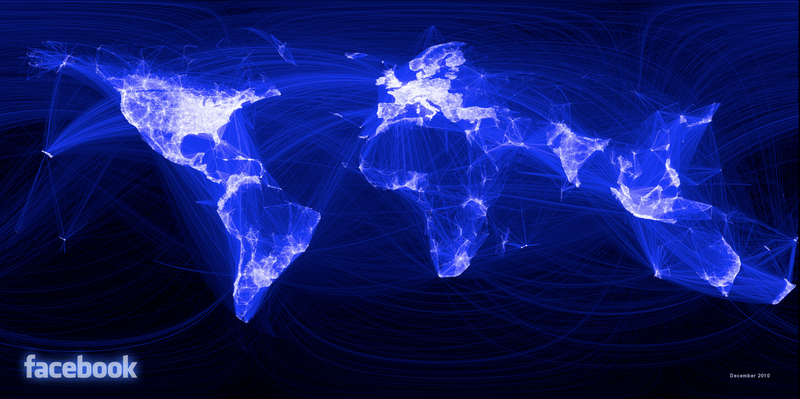
\includegraphics{facebook.png}
\caption{Figure 1: Facebook created this image with R to show how
Facebook connects the world.}
\end{figure}

\subsection{R or Python?}\label{r-or-python}

The world is quickly moving toward leveraging open source data science
tools rather than proprietary software. Over the last five years R and
Python have risen as the two primary open source tools used by data
professionals. While there is significant overlap in the capabilities of
both languages, in general the R Programming language is better at data
analysis and visualization, and Python is better at data acquisition and
producing code for production environments. We decided to teach R in
this class since it generally has better visualizations that support our
analysts as they tell the data narrative. Additionally, R is generally
more accessible across the Department of Defense.

\begin{figure}[htbp]
\centering
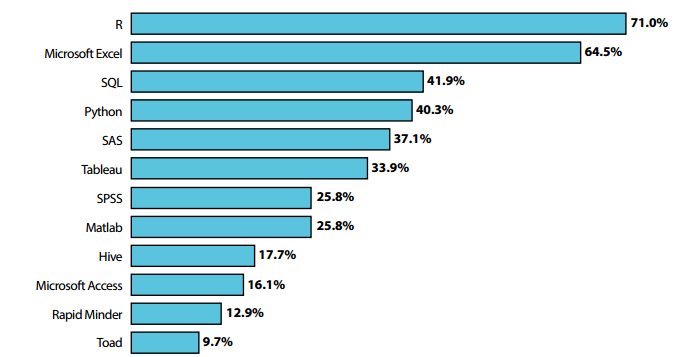
\includegraphics{whyR2.PNG}
\caption{Figure 2: LAVASTORM 2014 Survey of Industry: Primary tools used
by data scientists}
\end{figure}

R is open-source and is freely available to download. You can use base R
as-is to write and run R scripts. RStudio has provided a very useful
Integrated Development Environment (IDE) or ``front-end'' for R that is
generally easier to use (R is still the ``engine''; you can't run
RStudio without R). We will exclusively use RStudio in this course.

Note that you can also run R from a server in the ``cloud''. The US Army
\href{https://dscoe.army.mil/}{Data Science Center of Education (DSCOE)}
provides several tutorials that explain how to do this.

\begin{center}\rule{0.5\linewidth}{\linethickness}\end{center}

\section{Installation}\label{installation}

\begin{enumerate}
\def\labelenumi{\arabic{enumi}.}
\item
  Download and install the current version of R on CRAN.
\item
  Download and install the RStudio Desktop Open Source License by going
  to the RStudio Downloads page and selecting your operating system.
\end{enumerate}

\section{R Environment and Workspace}\label{r-environment-and-workspace}

Watach this brief introductory video to explore the RStudio interface:

R is always pointing to a specific directory (or folder) on your
computer. This is called your \emph{working directory}. R will always
directly read files and write files to this directory. You can see your
working directory by typing the \texttt{getwd()} command in the console:

\begin{Shaded}
\begin{Highlighting}[]
\KeywordTok{getwd}\NormalTok{()}
\end{Highlighting}
\end{Shaded}

\begin{verbatim}
## [1] "/home/rstudio/bookdown-demo-master"
\end{verbatim}

If you want to change where your working directory is, you can do this
three different ways. If you are using RStudio, you can go to
\emph{Session -\textgreater{} Set Working Directory}. You can also use
the \emph{Files} tab to navigate to your desired working directory, and
then click on \emph{More -\textgreater{} Set as Working Directory}. If
you want to change your \emph{working directory} using a command
(especially if you're using base R), then you can type the following:

\begin{Shaded}
\begin{Highlighting}[]
\KeywordTok{setwd}\NormalTok{(}\StringTok{"C:/Users/My.User.Name/Documents"}\NormalTok{)  }\CommentTok{#Make sure you use forward slashes in Windows}
\end{Highlighting}
\end{Shaded}

If you want to see the names of files in your working directory without
opening Windows Explorer, you can use the \texttt{dir()} command:

\begin{Shaded}
\begin{Highlighting}[]
\KeywordTok{dir}\NormalTok{()}
\end{Highlighting}
\end{Shaded}

\begin{verbatim}
##  [1] "01-fundamentals.Rmd"      "02-munging.Rmd"          
##  [3] "03-visualization.Rmd"     "04-control.Rmd"          
##  [5] "05-dates.Rmd"             "06-exam.Rmd"             
##  [7] "07-references.Rmd"        "apft.csv"                
##  [9] "_book"                    "book.bib"                
## [11] "bookdown-demo_files"      "bookdown-demo.Rmd"       
## [13] "bookdown-demo.Rproj"      "_bookdown_files"         
## [15] "_bookdown.yml"            "_build.sh"               
## [17] "ctx-10008"                "dataframe.PNG"           
## [19] "dataWrangling.jpg"        "DD508009"                
## [21] "_deploy.sh"               "DESCRIPTION"             
## [23] "dplyr.png"                "environment.PNG"         
## [25] "facebook.png"             "filterColumn.PNG"        
## [27] "filterRow.PNG"            "index.Rmd"               
## [29] "KoreanConflict.csv"       "LICENSE"                 
## [31] "list.PNG"                 "matrix.PNG"              
## [33] "notebooks"                "_output.yml"             
## [35] "packages.bib"             "pcs"                     
## [37] "per"                      "persistent-state"        
## [39] "preamble.tex"             "prerequisite-book.Rproj" 
## [41] "prop"                     "rating2.csv"             
## [43] "README.md"                "rmd-outputs"             
## [45] "s-6E3A07E1"               "saved_source_markers"    
## [47] "screen1.png"              "session-persistent-state"
## [49] "style.css"                "summer.csv"              
## [51] "tidyr.png"                "toc.css"                 
## [53] "vector.PNG"               "whyR2.PNG"               
## [55] "whyR.PNG"
\end{verbatim}

Note that \texttt{dir()} lists the names of the files in your working
directory, which saves you the time of opening up Windows Explorer to
remind yourself what you named your data file.

Before we get into the many types and shapes of data, let's first see
that your RStudio \emph{Console} (appears as the lower left pane in
RStudio by default) can execute commands just like a calculator:

\begin{Shaded}
\begin{Highlighting}[]
\DecValTok{5} \NormalTok{+}\StringTok{ }\DecValTok{4} \NormalTok{+}\StringTok{ }\DecValTok{7} \NormalTok{*}\StringTok{ }\DecValTok{7}
\end{Highlighting}
\end{Shaded}

\begin{verbatim}
## [1] 58
\end{verbatim}

or

\begin{Shaded}
\begin{Highlighting}[]
\NormalTok{pi *}\StringTok{ }\FloatTok{7.2}\NormalTok{^}\DecValTok{2}
\end{Highlighting}
\end{Shaded}

\begin{verbatim}
## [1] 162.8602
\end{verbatim}

Note that in both of these examples, the answer is printed to the
screen, but not stored in memory. In other words, I cannot access that
answer without redoing the calculation. If I want to store the result in
memory, then I assign the answer to a name. We use the symbol
\texttt{\textless{}-} to mean ``assign''. In other words, the result of
the computation on the right of the symbol is assigned to the name on
the left of the symbol. For example:

\begin{Shaded}
\begin{Highlighting}[]
\NormalTok{x <-}\StringTok{ }\DecValTok{4}\NormalTok{*}\DecValTok{4}
\end{Highlighting}
\end{Shaded}

I have now assigned the result of my computation to the name \texttt{x}.
If I want to see this value of \texttt{x} in the future, I can just type
it in the \emph{Console}.

\begin{Shaded}
\begin{Highlighting}[]
\NormalTok{x}
\end{Highlighting}
\end{Shaded}

\begin{verbatim}
## [1] 16
\end{verbatim}

I can also use it in future computations:

\begin{Shaded}
\begin{Highlighting}[]
\NormalTok{y <-}\StringTok{ }\NormalTok{x/}\DecValTok{2}
\end{Highlighting}
\end{Shaded}

The variable \texttt{y} is now stored in your \emph{Global Environment}
alongside the stored variable \texttt{x}. Think of the \emph{Global
Environment} as your ``workbench'' that contains all of the data and
values that you have ready for use. In RStudio, you can usually see what
is in your \emph{Global Environment} in the \emph{Environment} pane
(appears as a tab in the upper right pane by default).

\begin{figure}[htbp]
\centering
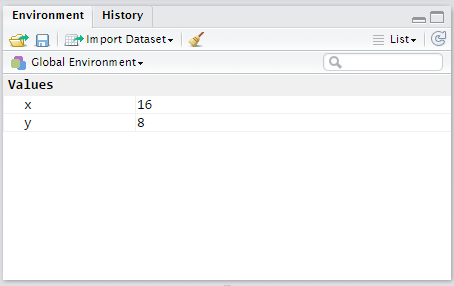
\includegraphics{environment.PNG}
\caption{Figure 3: The ``Environment'' pane shows the name and type of
data held in memory}
\end{figure}

If you're using base R, you can list the variables that are in your
\emph{Global Environment} using the \texttt{ls()} command:

\begin{Shaded}
\begin{Highlighting}[]
\KeywordTok{ls}\NormalTok{()}
\end{Highlighting}
\end{Shaded}

\begin{verbatim}
## [1] "x" "y"
\end{verbatim}

When you close either RStudio or base R, it will ask you if you want to
save your \emph{workspace}. It is essentially asking you if you want to
save what is on your workbench. If you choose ``yes'', then it will save
an \emph{.RData} file of everything that is in your workspace in your
working directory. If you restart R from this working directory, it will
load all of these items into your workspace. Generally it is not a good
idea to save your workspace as long as you have all of the code it would
take to quickly recreate all of the items in your workspace. However, if
you have some code that takes a long time to run, then it is best to
save these items in a workspace so that you don't have to wait hours or
even days a second time to recreate them. Generally your clean R code
takes only seconds to prepare your data for analysis, so it is best to
not save your workspace each time you close R or RStudio.

\section{Data Types}\label{data-types}

Now that we have R and RStudio installed, let's look at different
classes of data. The basic building blocks are the \emph{integer},
\emph{numeric}, \emph{character}, \emph{date}, \emph{boolean} (logical),
and \emph{factor} classes of data. The first four should be
self-explanatory, and examples of all four are below:

\begin{Shaded}
\begin{Highlighting}[]
\NormalTok{x <-}\StringTok{ }\DecValTok{4}                        \CommentTok{#integer}
\NormalTok{x <-}\StringTok{ }\FloatTok{4.56}                     \CommentTok{#numeric}
\NormalTok{x <-}\StringTok{ }\OtherTok{TRUE}                     \CommentTok{#boolean}
\NormalTok{x <-}\StringTok{ "Rangers Lead the Way!"}  \CommentTok{#character}
\end{Highlighting}
\end{Shaded}

Use the \texttt{class()} command to find out what type of data you have.
Note that because we were using \texttt{x} for all three, we were
writing over the value of \texttt{x}. At the end of running these four
lines of code, \texttt{x} would equal the last line of code: the
character string ``Rangers Lead the Way!''

\begin{Shaded}
\begin{Highlighting}[]
\KeywordTok{class}\NormalTok{(x)}
\end{Highlighting}
\end{Shaded}

\begin{verbatim}
## [1] "character"
\end{verbatim}

R does not automatically recognize \emph{date} data. When you read
\emph{date} data into R, it is initially converted to \emph{character}
data. If you want R to recognize it as a \emph{date}, you need to
explicity change it (we will go over this in more detail later):

\begin{Shaded}
\begin{Highlighting}[]
\NormalTok{x <-}\StringTok{ "2014-01-01"}
\KeywordTok{class}\NormalTok{(x)}
\end{Highlighting}
\end{Shaded}

\begin{verbatim}
## [1] "character"
\end{verbatim}

\begin{Shaded}
\begin{Highlighting}[]
\NormalTok{x <-}\StringTok{ }\KeywordTok{as.Date}\NormalTok{(x)}
\KeywordTok{class}\NormalTok{(x)}
\end{Highlighting}
\end{Shaded}

\begin{verbatim}
## [1] "Date"
\end{verbatim}

There is also a type of data called \emph{factor} data. This is
categorical data (often a character string) that has a numeric value
tied to it for certain types of models. Character data is often coerced
to the \emph{factor} class when you have nominal data (for example, a
\emph{gender} field that contained the strings ``male'' and ``female'').
If I change this into a factor, it will still be represented as ``male''
and ``female'', but it will also be represented numerically (as a 1 and
2). You need to be very careful when using factors, since many of the
functions in R can't handle factor data. You can see the use of factor
data below:

\begin{Shaded}
\begin{Highlighting}[]
\NormalTok{y <-}\StringTok{ }\KeywordTok{c}\NormalTok{(}\StringTok{"male"}\NormalTok{,}\StringTok{"male"}\NormalTok{,}\StringTok{"female"}\NormalTok{,}\StringTok{"male"}\NormalTok{,}\StringTok{"female"}\NormalTok{)}
\end{Highlighting}
\end{Shaded}

This is character data. If I tried to plot \texttt{y} right now, R would
show an error, since you can't print \emph{character} data. Lets convert
this to a factor now:

\begin{Shaded}
\begin{Highlighting}[]
\NormalTok{y <-}\StringTok{ }\KeywordTok{as.factor}\NormalTok{(y)}
\NormalTok{y}
\end{Highlighting}
\end{Shaded}

\begin{verbatim}
## [1] male   male   female male   female
## Levels: female male
\end{verbatim}

Now we can try to plot \texttt{y}:

\begin{Shaded}
\begin{Highlighting}[]
\KeywordTok{plot}\NormalTok{(y)}
\end{Highlighting}
\end{Shaded}

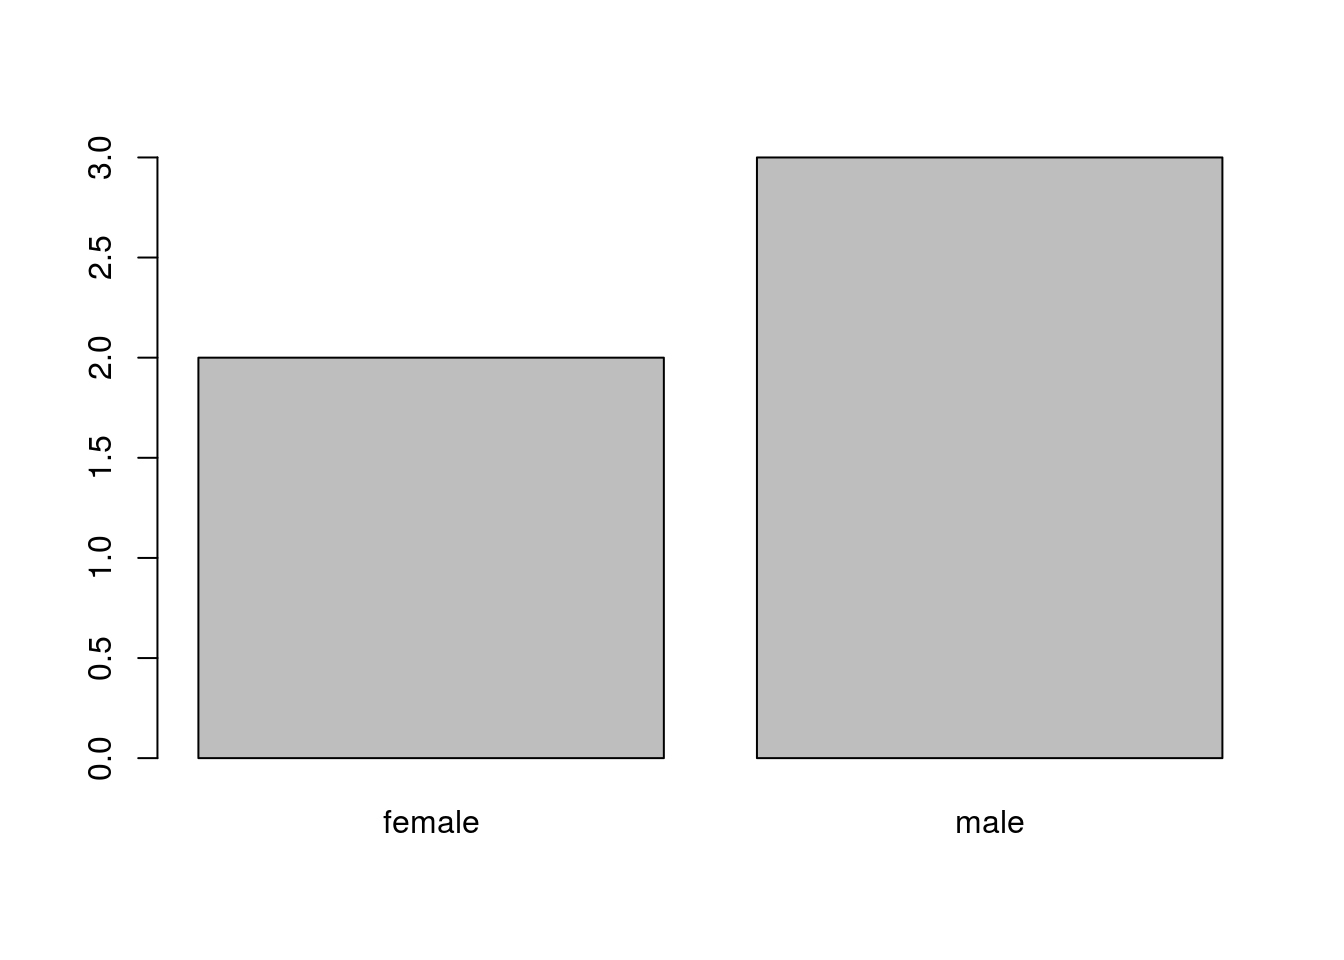
\includegraphics{bookdown-demo_files/figure-latex/unnamed-chunk-16-1.pdf}

It plots a barchart because R recognizes \texttt{y} as a factor and has
a numeric value associated with both of the ``levels'' in the factor.

\section{Data Structures}\label{data-structures}

The data that we showed above is trivial (and very small) data. To work
with larger data, we'd prefer to have it organized into a usable data
structure. In this section we will introduce you to the four primary
data structures that we will use:

\begin{longtable}[]{@{}ll@{}}
\toprule
\begin{minipage}[b]{0.18\columnwidth}\raggedright\strut
Data Structure\strut
\end{minipage} & \begin{minipage}[b]{0.24\columnwidth}\raggedright\strut
Definition\strut
\end{minipage}\tabularnewline
\midrule
\endhead
\begin{minipage}[t]{0.18\columnwidth}\raggedright\strut
Vector\strut
\end{minipage} & \begin{minipage}[t]{0.24\columnwidth}\raggedright\strut
Data in one dimension\strut
\end{minipage}\tabularnewline
\begin{minipage}[t]{0.18\columnwidth}\raggedright\strut
Data Frame\strut
\end{minipage} & \begin{minipage}[t]{0.24\columnwidth}\raggedright\strut
Two-dimensional data (most commonly used data structure)\strut
\end{minipage}\tabularnewline
\begin{minipage}[t]{0.18\columnwidth}\raggedright\strut
List\strut
\end{minipage} & \begin{minipage}[t]{0.24\columnwidth}\raggedright\strut
A one-dimensional data structure that can contain any class of data
(objects could be other data structures)\strut
\end{minipage}\tabularnewline
\begin{minipage}[t]{0.18\columnwidth}\raggedright\strut
Matrix\strut
\end{minipage} & \begin{minipage}[t]{0.24\columnwidth}\raggedright\strut
Multi-dimensional data of the same class\strut
\end{minipage}\tabularnewline
\bottomrule
\end{longtable}

Data types can also be described by the dimensionality of the data they
can handle. So far we've been using \emph{scalars}, in which our
variable \texttt{x} is a single value. Data can have 1, 2, or even more
dimensions if required.

\subsection{Vector Data Structure}\label{vector-data-structure}

One-dimensional data that is of the same class is often organized into a
\emph{vector}. All objects in a vector must be of the same class (or
will be coerced to the same class). A picture of a vector is given
below:

\begin{figure}[htbp]
\centering
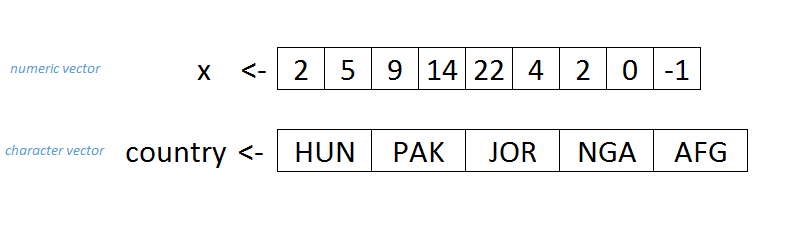
\includegraphics{vector.PNG}
\caption{Figure 4: Understanding the ``Vector'' Data Structure in R}
\end{figure}

An example of creating a vector in R is given below:

\begin{Shaded}
\begin{Highlighting}[]
\NormalTok{x<-}\KeywordTok{c}\NormalTok{(}\DecValTok{1}\NormalTok{,}\DecValTok{6}\NormalTok{,}\DecValTok{3}\NormalTok{,}\DecValTok{9}\NormalTok{,}\DecValTok{8}\NormalTok{,}\DecValTok{2}\NormalTok{)    ## "c" means combine the values into a vector}
\end{Highlighting}
\end{Shaded}

If you need to create a vector of sequential integers, you can use a
colon:

\begin{Shaded}
\begin{Highlighting}[]
\NormalTok{x <-}\StringTok{ }\DecValTok{1}\NormalTok{:}\DecValTok{10}
\NormalTok{x}
\end{Highlighting}
\end{Shaded}

\begin{verbatim}
##  [1]  1  2  3  4  5  6  7  8  9 10
\end{verbatim}

If you need to create a vector of a specific sequence, you can use the
sequence command:

\begin{Shaded}
\begin{Highlighting}[]
\NormalTok{x <-}\StringTok{ }\KeywordTok{seq}\NormalTok{(}\DataTypeTok{from=}\DecValTok{2}\NormalTok{, }\DataTypeTok{to=}\DecValTok{20}\NormalTok{, }\DataTypeTok{by=}\DecValTok{6}\NormalTok{)}
\NormalTok{x}
\end{Highlighting}
\end{Shaded}

\begin{verbatim}
## [1]  2  8 14 20
\end{verbatim}

If you need to create a vector of the same number, you can use the
repeat command:

\begin{Shaded}
\begin{Highlighting}[]
\NormalTok{x <-}\StringTok{ }\KeywordTok{rep}\NormalTok{(}\DecValTok{1}\NormalTok{,}\DecValTok{10}\NormalTok{)  }\CommentTok{# Repeat 1 ten times}
\NormalTok{x}
\end{Highlighting}
\end{Shaded}

\begin{verbatim}
##  [1] 1 1 1 1 1 1 1 1 1 1
\end{verbatim}

\subsection{Data Frame Data Structure}\label{data-frame-data-structure}

Anyone who has used Microsoft Excel is used to seeing data in the
traditional two dimensional table. R's ``data frame'' structures data in
this way. A picture of a data frame is provided below:

\begin{figure}[htbp]
\centering
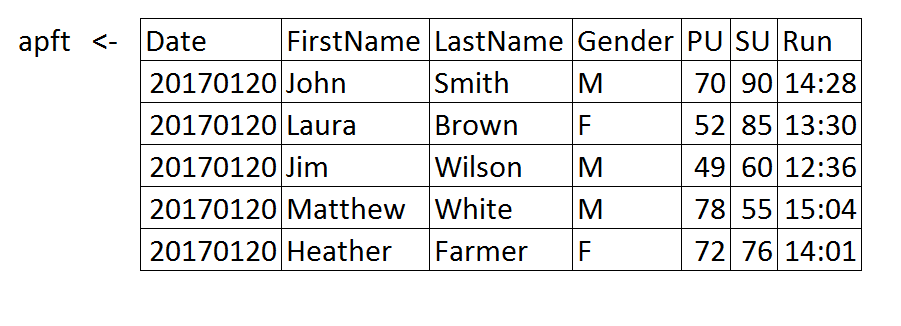
\includegraphics{dataframe.PNG}
\caption{Figure 5: Understanding the ``Data Frame''" Structure in R}
\end{figure}

Each column of a data frame is a vector, and each vector must have the
same class of data. A data frame is a list of vectors where each each
vector has the same length. A data frame is usually created when you
read data from an external file (usually a CSV file), but you can also
create one manually, as seen below:

\begin{Shaded}
\begin{Highlighting}[]
\NormalTok{##Create a data frame}
\NormalTok{apft <-}\StringTok{ }\KeywordTok{data.frame}\NormalTok{(}\DataTypeTok{Name =} \KeywordTok{c}\NormalTok{(}\StringTok{"John"}\NormalTok{,}\StringTok{"Laura"}\NormalTok{,}\StringTok{"Jim"}\NormalTok{),}
                   \DataTypeTok{Gender =} \KeywordTok{c}\NormalTok{(}\StringTok{"M"}\NormalTok{,}\StringTok{"F"}\NormalTok{,}\StringTok{"M"}\NormalTok{),}
                   \DataTypeTok{PU =} \KeywordTok{c}\NormalTok{(}\DecValTok{70}\NormalTok{, }\DecValTok{52}\NormalTok{, }\DecValTok{49}\NormalTok{),}
                   \DataTypeTok{SU =} \KeywordTok{c}\NormalTok{(}\DecValTok{90}\NormalTok{, }\DecValTok{85}\NormalTok{, }\DecValTok{60}\NormalTok{),}
                   \DataTypeTok{Run =} \KeywordTok{c}\NormalTok{(}\StringTok{"14:28"}\NormalTok{,}\StringTok{"13:30"}\NormalTok{,}\StringTok{"12:36"}\NormalTok{))}
\NormalTok{##Print object}
\NormalTok{apft}
\end{Highlighting}
\end{Shaded}

\begin{verbatim}
##    Name Gender PU SU   Run
## 1  John      M 70 90 14:28
## 2 Laura      F 52 85 13:30
## 3   Jim      M 49 60 12:36
\end{verbatim}

It is often the case that you might want to extract a subset of your
data frame.

If you want just one element from the data frame, we can specify which
row and which column to keep.

\begin{Shaded}
\begin{Highlighting}[]
\NormalTok{apft[}\DecValTok{3}\NormalTok{,}\DecValTok{1}\NormalTok{] }\CommentTok{#This returns the 3rd row, 1st column.}
\end{Highlighting}
\end{Shaded}

\begin{verbatim}
## [1] Jim
## Levels: Jim John Laura
\end{verbatim}

If you want more than one element from the data frame, we can specify
which row(s) and which column(s) to keep.

\begin{Shaded}
\begin{Highlighting}[]
\NormalTok{apft[}\DecValTok{2}\NormalTok{:}\DecValTok{3}\NormalTok{,}\DecValTok{1}\NormalTok{:}\DecValTok{2}\NormalTok{] }\CommentTok{#This returns the 2nd and 3rd rows, 1st and 2nd columns.}
\end{Highlighting}
\end{Shaded}

\begin{verbatim}
##    Name Gender
## 2 Laura      F
## 3   Jim      M
\end{verbatim}

If you want just a few rows, we can specify which rows to keep.

\begin{Shaded}
\begin{Highlighting}[]
\NormalTok{apft[}\DecValTok{3}\NormalTok{,] }\CommentTok{#This returns the 3rd row, all columns.}
\end{Highlighting}
\end{Shaded}

\begin{verbatim}
##   Name Gender PU SU   Run
## 3  Jim      M 49 60 12:36
\end{verbatim}

If you want just a few columns, we can specify which columns to keep.

\begin{Shaded}
\begin{Highlighting}[]
\NormalTok{apft[,}\DecValTok{1}\NormalTok{] }\CommentTok{#This returns all rows, first column.}
\end{Highlighting}
\end{Shaded}

\begin{verbatim}
## [1] John  Laura Jim  
## Levels: Jim John Laura
\end{verbatim}

Extracting one column in a data frame is typically accomplished with the
\texttt{\$} operator.

\begin{Shaded}
\begin{Highlighting}[]
\NormalTok{apft$Name}
\end{Highlighting}
\end{Shaded}

\begin{verbatim}
## [1] John  Laura Jim  
## Levels: Jim John Laura
\end{verbatim}

\subsection{List Data Structure}\label{list-data-structure}

A list is a linear container for objects of any class or data structure.
Each object in a list is separate and distinct.

A list is helpful in several situations. For example, there are times
you might have vectors that do not all have the same length. For
example, lets say we extracted hashtags from tweets at the Rio Olympics.
The number of hashtags per tweet can range from zero to seven or eight
(see Figure 6 below).

\begin{figure}[htbp]
\centering
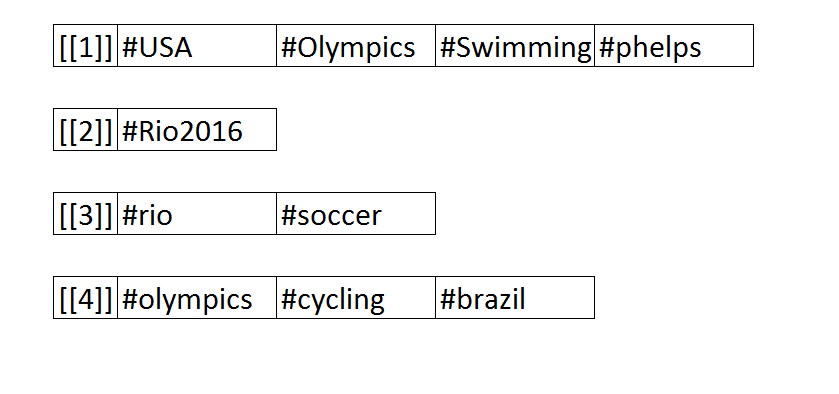
\includegraphics{list.PNG}
\caption{Figure 6: Understanding the ``List''" Data Structure in R}
\end{figure}

You can't store these vectors in a data frame because they aren't the
same length. A list is the appropriate object to store these vectors. A
list is also helpful for storing different types of data in a single
object. For example, we can store a scalar, a data frame, and a vector
in a single list:

\begin{Shaded}
\begin{Highlighting}[]
\NormalTok{##Store a scalar, vector, and data frame in a list}
\NormalTok{myList <-}\StringTok{ }\KeywordTok{list}\NormalTok{(y, x, apft)}

\NormalTok{##Print object}
\NormalTok{myList}
\end{Highlighting}
\end{Shaded}

\begin{verbatim}
## [[1]]
## [1] male   male   female male   female
## Levels: female male
## 
## [[2]]
##  [1] 1 1 1 1 1 1 1 1 1 1
## 
## [[3]]
##    Name Gender PU SU   Run
## 1  John      M 70 90 14:28
## 2 Laura      F 52 85 13:30
## 3   Jim      M 49 60 12:36
\end{verbatim}

Lists also create a great container for reading multiple data files into
R and combining them into a single data frame.

\subsection{Matrix Data Structure}\label{matrix-data-structure}

While matrices exist as an important data structure in R, we will not
use the matrix structure often in this course. A matrix is a
multi-dimensional array of numeric, boolean, or integer data (NOT
character, date, or factor data).

\begin{figure}[htbp]
\centering
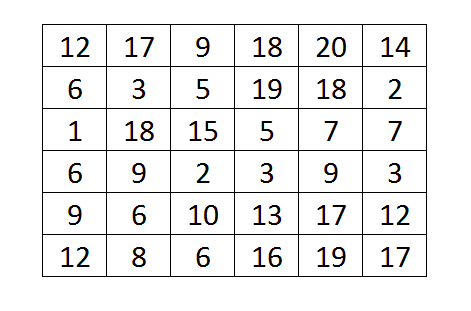
\includegraphics{matrix.PNG}
\caption{Figure 7: Understanding the ``Matrix'' Data Structure in R}
\end{figure}

Below is an example of creating a matrix object in R:

\begin{Shaded}
\begin{Highlighting}[]
\NormalTok{## Create a 2x3 matrix filling row by row.}
\NormalTok{mdat <-}\StringTok{ }\KeywordTok{matrix}\NormalTok{(}\KeywordTok{c}\NormalTok{(}\DecValTok{1}\NormalTok{,}\DecValTok{2}\NormalTok{,}\DecValTok{3}\NormalTok{, }\DecValTok{11}\NormalTok{,}\DecValTok{12}\NormalTok{,}\DecValTok{13}\NormalTok{), }\DataTypeTok{nrow =} \DecValTok{2}\NormalTok{, }\DataTypeTok{ncol =} \DecValTok{3}\NormalTok{, }\DataTypeTok{byrow =} \OtherTok{TRUE}\NormalTok{)}

\NormalTok{##Print object}
\NormalTok{mdat}
\end{Highlighting}
\end{Shaded}

\begin{verbatim}
##      [,1] [,2] [,3]
## [1,]    1    2    3
## [2,]   11   12   13
\end{verbatim}

With the exception of the \texttt{\$} operator, matrices are indexed in
the same way as data frames. As mentioned previously, we will not use
matrices much in this course.

\section{Input/Output Data}\label{inputoutput-data}

Let's now learn how to read and write data. To do this with some fun
data, let's read in some data on movie ratings. This data contains users
that rated movies in 2015. Each record (or row) represents a single user
rating a single movie. Movies can have more than one rating, and users
can rate more than one movie. Make sure you download the data at
\url{https://s3.amazonaws.com/dscoe-data/rating2.csv} and follow along
with this tutorial.

Note: if you're using a cloud environment, you can download the data by
running the following command:

\begin{Shaded}
\begin{Highlighting}[]
\KeywordTok{download.file}\NormalTok{(}\StringTok{"https://s3.amazonaws.com/dscoe-data-2/rating2.csv"}\NormalTok{, }\DataTypeTok{destfile =} \StringTok{"rating2.csv"}\NormalTok{)}
\end{Highlighting}
\end{Shaded}

We use the command \emph{read.csv} to read in data. We also make sure to
assign this to an object name (in this case, the object name is
\texttt{rating}).

\begin{Shaded}
\begin{Highlighting}[]
\NormalTok{rating <-}\StringTok{ }\KeywordTok{read.csv}\NormalTok{(}\StringTok{"rating2.csv"}\NormalTok{, }\DataTypeTok{as.is =} \OtherTok{TRUE}\NormalTok{)}
\end{Highlighting}
\end{Shaded}

The \texttt{as.is\ =\ TRUE} parameter ensures that any character data is
formatted into a \emph{character} vector rather than a \emph{factor}
vector. You can always convert from the provided character strings to
another data type, but using \texttt{as.is=TRUE} ensures you know your
starting point. One example where the factor interpretation is
particularly problematic involves working with dates.

Now that we've read the file in, we'll briefly explore this data object
with a few helpful commands. One of the most powerful commands to
explore any object is the structure command \texttt{str()}. This command
gives the overall size of the object (in this case it has 283,886 rows
and 7 columns), as well as the class of each column vector and the first
few observations from each column vector.

\begin{Shaded}
\begin{Highlighting}[]
\CommentTok{# The structure command prints the structure of the data object.}
\KeywordTok{str}\NormalTok{(rating)}
\end{Highlighting}
\end{Shaded}

\begin{verbatim}
## 'data.frame':    283886 obs. of  7 variables:
##  $ userId   : int  31 31 31 31 31 31 31 31 31 31 ...
##  $ movieId  : int  1 110 260 364 527 588 594 616 1196 1197 ...
##  $ rating   : num  3 5 5 3 0.5 3 2.5 4 5 3 ...
##  $ timestamp: chr  "2015-02-23 23:18:07" "2015-02-23 23:17:53" "2015-02-23 23:17:13" "2015-02-25 06:13:27" ...
##  $ year     : int  2015 2015 2015 2015 2015 2015 2015 2015 2015 2015 ...
##  $ title    : chr  "Toy Story (1995)" "Braveheart (1995)" "Star Wars: Episode IV - A New Hope (1977)" "Lion King, The (1994)" ...
##  $ genres   : chr  "Adventure|Animation|Children|Comedy|Fantasy" "Action|Drama|War" "Action|Adventure|Sci-Fi" "Adventure|Animation|Children|Drama|Musical|IMAX" ...
\end{verbatim}

Related to the \texttt{str()} command is the \texttt{summary()} command.
This command is especially helpful if you have numeric data in the
object and you want to view some of the basic statistics regarding this
data.

\begin{Shaded}
\begin{Highlighting}[]
\CommentTok{# The summary command prints summary statistics about an object in memory.}
\KeywordTok{summary}\NormalTok{(rating)}
\end{Highlighting}
\end{Shaded}

\begin{verbatim}
##      userId          movieId           rating     timestamp        
##  Min.   :    31   Min.   :     1   Min.   :0.5   Length:283886     
##  1st Qu.: 34847   1st Qu.:  2712   1st Qu.:3.0   Class :character  
##  Median : 69852   Median :  8644   Median :3.5   Mode  :character  
##  Mean   : 69325   Mean   : 39896   Mean   :3.5                     
##  3rd Qu.:104000   3rd Qu.: 79132   3rd Qu.:4.0                     
##  Max.   :138414   Max.   :131262   Max.   :5.0                     
##       year         title              genres         
##  Min.   :2015   Length:283886      Length:283886     
##  1st Qu.:2015   Class :character   Class :character  
##  Median :2015   Mode  :character   Mode  :character  
##  Mean   :2015                                        
##  3rd Qu.:2015                                        
##  Max.   :2015
\end{verbatim}

You can also use the command \texttt{head()} to print only the first 6
rows. This gives titles of the variables (columns) as well as a feel for
the data:

\begin{Shaded}
\begin{Highlighting}[]
\CommentTok{# The head command prints the first six rows of the data set.}
\KeywordTok{head}\NormalTok{(rating)}
\end{Highlighting}
\end{Shaded}

\begin{verbatim}
##   userId movieId rating           timestamp year
## 1     31       1    3.0 2015-02-23 23:18:07 2015
## 2     31     110    5.0 2015-02-23 23:17:53 2015
## 3     31     260    5.0 2015-02-23 23:17:13 2015
## 4     31     364    3.0 2015-02-25 06:13:27 2015
## 5     31     527    0.5 2015-02-23 23:19:58 2015
## 6     31     588    3.0 2015-02-25 05:41:09 2015
##                                       title
## 1                          Toy Story (1995)
## 2                         Braveheart (1995)
## 3 Star Wars: Episode IV - A New Hope (1977)
## 4                     Lion King, The (1994)
## 5                   Schindler's List (1993)
## 6                            Aladdin (1992)
##                                            genres
## 1     Adventure|Animation|Children|Comedy|Fantasy
## 2                                Action|Drama|War
## 3                         Action|Adventure|Sci-Fi
## 4 Adventure|Animation|Children|Drama|Musical|IMAX
## 5                                       Drama|War
## 6     Adventure|Animation|Children|Comedy|Musical
\end{verbatim}

If you only want to print the names of the columns, use the
\texttt{names()} command:

\begin{Shaded}
\begin{Highlighting}[]
\CommentTok{# The names command just prints the column names of a data frame.}
\KeywordTok{names}\NormalTok{(rating)}
\end{Highlighting}
\end{Shaded}

\begin{verbatim}
## [1] "userId"    "movieId"   "rating"    "timestamp" "year"      "title"    
## [7] "genres"
\end{verbatim}

Finally, if we only want the dimensions of the data, we can use
\texttt{dim()} to get all of the dimensions, \texttt{nrow()} to access
the number of rows, and \texttt{ncol()} to access the number of columns:

\begin{Shaded}
\begin{Highlighting}[]
\CommentTok{# The dim command prints the dimensions of the object.}
\KeywordTok{dim}\NormalTok{(rating)}
\end{Highlighting}
\end{Shaded}

\begin{verbatim}
## [1] 283886      7
\end{verbatim}

\begin{Shaded}
\begin{Highlighting}[]
\CommentTok{# The nrow command prints the number of rows of a data frame.}
\KeywordTok{nrow}\NormalTok{(rating)}
\end{Highlighting}
\end{Shaded}

\begin{verbatim}
## [1] 283886
\end{verbatim}

\begin{Shaded}
\begin{Highlighting}[]
\CommentTok{# The ncol command prints the number of columns of a data frame.}
\KeywordTok{ncol}\NormalTok{(rating)}
\end{Highlighting}
\end{Shaded}

\begin{verbatim}
## [1] 7
\end{verbatim}

\section{Getting Help}\label{getting-help}

There are several ways to get help in R. The \texttt{help()} function
and the \texttt{?} function can access the documentation for packages
and functions that you have loaded into R. \texttt{help.search} and the
\texttt{??} function both search within the R documentation and any
loaded packages. Additionally, you can use the \texttt{args()} function
to print out the arguments for a function.

\begin{Shaded}
\begin{Highlighting}[]
\CommentTok{# Getting help for the str function}
\KeywordTok{help}\NormalTok{(str)}

\CommentTok{# or}
\NormalTok{?str}

\CommentTok{# Searching within documentation for "subset"}
\KeywordTok{help.search}\NormalTok{(}\StringTok{'subset'}\NormalTok{)}

\CommentTok{# or}
\NormalTok{??subset}
\end{Highlighting}
\end{Shaded}

\section{Practice Problem}\label{practice-problem}

Download the Korean War Casualty Data by downloading the Comma Separated
Value (CSV) file here:

\url{https://s3.amazonaws.com/dscoe-data/KoreanConflict.csv}

If you're using a cloud environment, you can download the data by
running the following command:

\begin{Shaded}
\begin{Highlighting}[]
\KeywordTok{download.file}\NormalTok{(}\StringTok{"https://s3.amazonaws.com/dscoe-data-2/KoreanConflict.csv"}\NormalTok{, }\DataTypeTok{destfile =} \StringTok{"KoreanConflict.csv"}\NormalTok{)}
\end{Highlighting}
\end{Shaded}

Read the file \texttt{KoreanConflict.csv} into your R environment.
Explore the data using the commands that we learned during this lesson.
At this point, you should be able to discover the following:

\begin{enumerate}
\def\labelenumi{\arabic{enumi}.}
\tightlist
\item
  How many observations (rows) are in your Korean Conflict data frame?
\item
  How many variables (columns) describe each observation?
\item
  Which column of your data frame describes an individual's duty
  position? (Hint: Try adding a \texttt{\$} after the name of your data
  frame to access a specific column of data.)
\item
  What is the range of birth years in your Korean Conflict data frame?
  (Hint: Use the \texttt{min()} and \texttt{max()} functions on the
  appropriate column.)
\end{enumerate}

\chapter{Basic Data Manipulation}\label{basic-data-manipulation}

The most time-intensive task in any data science endeavor is often
pre-processing the data. Real world data is often complex and messy.
Data processing (sometimes called ``munging'' or ``data wrangling'')
cleans and manipulates data so that it is in a form that is useful for
models and visualizations. The R programming language is one of the best
tools for manipulating data. This lesson will discuss the basics of data
structure as well as ways to subset, extract and otherwise manipulate
data.

\begin{figure}[htbp]
\centering
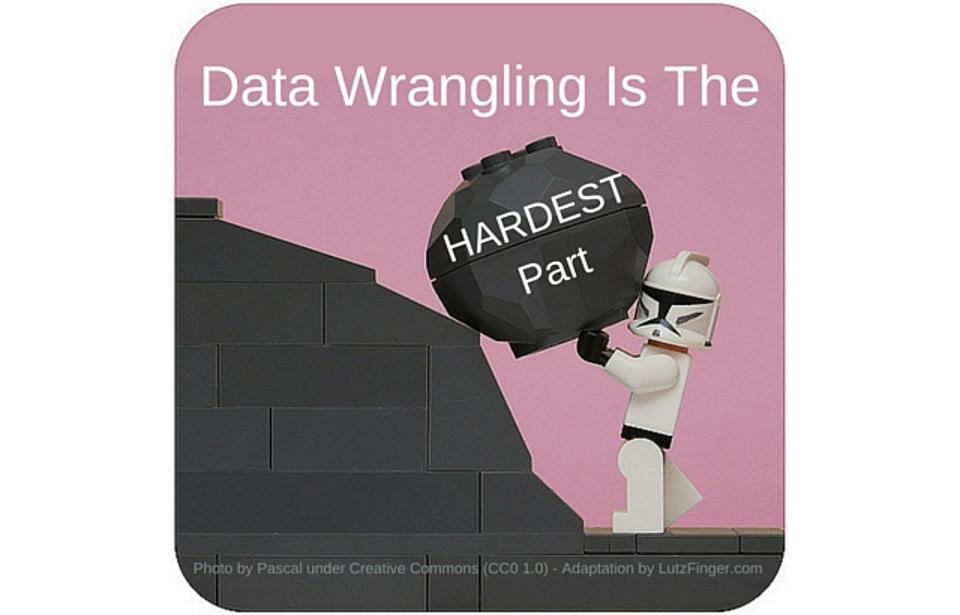
\includegraphics{dataWrangling.jpg}
\caption{Figure 1: ``Data Wrangling''" is often the most difficult part
of data science}
\end{figure}

\section{Data}\label{data}

For this lesson we will use casualty data from the Korean War. This data
set and many other interesting data sets are available at Kaggle. You
should have downloaded this data for the practice problem in Lesson 1.
First, let's read the data into R:

\begin{Shaded}
\begin{Highlighting}[]
\NormalTok{kor <-}\StringTok{ }\KeywordTok{read.csv}\NormalTok{(}\StringTok{"KoreanConflict.csv"}\NormalTok{, }\DataTypeTok{as.is =} \OtherTok{TRUE}\NormalTok{)}
\end{Highlighting}
\end{Shaded}

Now let's explore the data with some of the tools we learned in Lesson
1. First, let's look at the structure of the data:

\begin{Shaded}
\begin{Highlighting}[]
\KeywordTok{str}\NormalTok{(kor)  }\CommentTok{# Print the structure of the Korean Casualty Data.}
\end{Highlighting}
\end{Shaded}

\begin{verbatim}
## 'data.frame':    36574 obs. of  25 variables:
##  $ SERVICE_TYPE        : chr  "V" "R" "R" "V" ...
##  $ SERVICE_CODE        : chr  "L" "K" "K" "L" ...
##  $ ENROLLMENT          : chr  "ACTIVE - GUARD/RESERVE" "ACTIVE - REGULAR" "ACTIVE - REGULAR" "ACTIVE - GUARD/RESERVE" ...
##  $ BRANCH              : chr  "AIR FORCE" "ARMY" "ARMY" "ARMY" ...
##  $ RANK                : chr  "CAPT" "PVT" "PFC" "2LT" ...
##  $ PAY_GRADE           : chr  "O03" "E02" "E03" "O01" ...
##  $ POSITION            : chr  "" "FOOD SERVICE APPRENTICE" "HEAVY WEAPONS INFANTRYMAN" "INFANTRY UNIT COMMANDER" ...
##  $ BIRTH_YEAR          : chr  "1917" "1927" "1932" "1929" ...
##  $ SEX                 : chr  "M" "M" "M" "M" ...
##  $ HOME_CITY           : chr  "NEW YORK" "UNKNOWN" "UNKNOWN" "UNKNOWN" ...
##  $ HOME_COUNTY         : chr  "NEW YORK" "OCONEE" "BIBB" "COAHOMA" ...
##  $ NATIONALITY         : chr  "US" "US" "US" "US" ...
##  $ STATE_CODE          : chr  "NY" "GA" "GA" "MS" ...
##  $ HOME_STATE          : chr  "NEW YORK" "GEORGIA" "GEORGIA" "MISSISSIPPI" ...
##  $ MARITAL_STATUS      : chr  "MARRIED" "UNKNOWN" "UNKNOWN" "UNKNOWN" ...
##  $ ETHNICITY           : chr  "WHITE" "WHITE" "WHITE" "WHITE" ...
##  $ ETHNICITY_1         : chr  "NOT SPECIFIED" "NOT SPECIFIED" "NOT SPECIFIED" "NOT SPECIFIED" ...
##  $ ETHNICITY_2         : chr  "WHITE" "WHITE" "WHITE" "WHITE" ...
##  $ DIVISION            : chr  "93 BOMB SQ 19 BOMB GP" "29 RGT CMBT TEAM" "5 RGT 1 CAV DIV" "32 INF 7 DIV" ...
##  $ INCIDENT_DATE       : chr  "19510412" "19500727" "19510316" "19530122" ...
##  $ FATALITY_YEAR       : chr  "1951" "1950" "1951" "1953" ...
##  $ FATALITY_DATE       : chr  "20010402" "19500727" "19510316" "19530122" ...
##  $ HOSTILITY_CONDITIONS: chr  "H" "H" "H" "H" ...
##  $ FATALITY            : chr  "DECLARED DEAD" "KILLED IN ACTION" "KILLED IN ACTION" "KILLED IN ACTION" ...
##  $ BURIAL_STATUS       : chr  "Y" "Y" "Y" "Y" ...
\end{verbatim}

We see that this data has 36,574 rows and 25 columns. It appears that
each row of the data represents an individual service member who died in
the Korean War. Note that every single column is a \emph{character}
vector. This includes the rows like \texttt{BIRTH\_YEAR} and
\texttt{INCIDENT\_DATE} that appear like they should be numeric (the
fact that they are character means that at least one entry in this
column has \emph{alphabetic letters} rather than \emph{numbers}).

\section{Cell-level Data Access}\label{cell-level-data-access}

Let's briefly review some common indexing techniques for data frames.
This data set contains two dimensions (rows and columns). To access
specific rows and columns in R, we use the \emph{{[}row,column{]}}
format. For example, to access the data in the first row and first
column of our Korean Conflict data, we would use:

\begin{Shaded}
\begin{Highlighting}[]
\NormalTok{kor[}\DecValTok{1}\NormalTok{,}\DecValTok{1}\NormalTok{]  }\CommentTok{# First row, first column.}
\end{Highlighting}
\end{Shaded}

\begin{verbatim}
## [1] "V"
\end{verbatim}

If we want to access the first 5 entries from the first column, we would
use:

\begin{Shaded}
\begin{Highlighting}[]
\NormalTok{kor[}\DecValTok{1}\NormalTok{:}\DecValTok{5}\NormalTok{,}\DecValTok{1}\NormalTok{] }\CommentTok{# First five entries from the first column.}
\end{Highlighting}
\end{Shaded}

\begin{verbatim}
## [1] "V" "R" "R" "V" "R"
\end{verbatim}

If we want to access the first three rows from the 1st, 3rd, and 8th
column, we use the following format:

\begin{Shaded}
\begin{Highlighting}[]
\NormalTok{kor[}\DecValTok{1}\NormalTok{:}\DecValTok{3}\NormalTok{,}\KeywordTok{c}\NormalTok{(}\DecValTok{1}\NormalTok{,}\DecValTok{3}\NormalTok{,}\DecValTok{8}\NormalTok{)] }\CommentTok{# First three rows, columns 1, 3, and 8.}
\end{Highlighting}
\end{Shaded}

\begin{verbatim}
##   SERVICE_TYPE             ENROLLMENT BIRTH_YEAR
## 1            V ACTIVE - GUARD/RESERVE       1917
## 2            R       ACTIVE - REGULAR       1927
## 3            R       ACTIVE - REGULAR       1932
\end{verbatim}

If you want a subset of the rows and all columns, we can simply specify
which row(s) to keep.

\begin{Shaded}
\begin{Highlighting}[]
\NormalTok{kor[}\DecValTok{3}\NormalTok{,] }\CommentTok{# This returns the 3rd row, all 25 columns.}
\end{Highlighting}
\end{Shaded}

If you want all rows and a subset of the columns, we can simply specify
which columns to keep.

\begin{Shaded}
\begin{Highlighting}[]
\NormalTok{kor[,}\DecValTok{1}\NormalTok{] }\CommentTok{# This returns all 36,574 rows, first column.}
\end{Highlighting}
\end{Shaded}

Extracting one column in a data frame is typically accomplished with the
\texttt{\$} operator.

\begin{Shaded}
\begin{Highlighting}[]
\NormalTok{kor$RANK }\CommentTok{# This returns all 36,574 ranks.}
\end{Highlighting}
\end{Shaded}

You can also use multiple column names (or headers) to extract data from
specific columns. This is especially helpful if you can't remember
respective column numbers, or if you think the column order will ever
change. To extract the first three rows of data from \texttt{BRANCH},
\texttt{RANK}, and \texttt{HOME\_STATE}, we can use the code below:

\begin{Shaded}
\begin{Highlighting}[]
\NormalTok{kor[}\DecValTok{1}\NormalTok{:}\DecValTok{3}\NormalTok{,}\KeywordTok{c}\NormalTok{(}\StringTok{"RANK"}\NormalTok{,}\StringTok{"BRANCH"}\NormalTok{,}\StringTok{"HOME_STATE"}\NormalTok{)]}
\end{Highlighting}
\end{Shaded}

\begin{verbatim}
##   RANK    BRANCH HOME_STATE
## 1 CAPT AIR FORCE   NEW YORK
## 2  PVT      ARMY    GEORGIA
## 3  PFC      ARMY    GEORGIA
\end{verbatim}

Remember that each column represents a vector. In addition to the method
we just showed, you can access data from each column vector with the
following command:

\begin{Shaded}
\begin{Highlighting}[]
\NormalTok{kor$RANK[}\DecValTok{1}\NormalTok{:}\DecValTok{5}\NormalTok{]  }\CommentTok{# Prints the first five entries in RANK vector.}
\end{Highlighting}
\end{Shaded}

\begin{verbatim}
## [1] "CAPT" "PVT"  "PFC"  "2LT"  "CPL"
\end{verbatim}

The command above selects the RANK column from the \texttt{kor} data
frame and then prints to the screen the first five entries of this
column.

\section{\texorpdfstring{\texttt{table()} Command (and an example of
data
``cleaning'')}{table() Command (and an example of data cleaning)}}\label{table-command-and-an-example-of-data-cleaning}

Let's explore the data a bit more. The \texttt{table()} command provides
a great way to see all of the possible entries in categorical data. The
table command has similar functionality to \emph{Pivot Tables} in Excel,
but is much easier to use. To illustrate this command, we will table the
\texttt{BIRTH\_YEAR}.

\begin{Shaded}
\begin{Highlighting}[]
\KeywordTok{table}\NormalTok{(kor$BIRTH_YEAR) }\CommentTok{# Table BIRTH_YEAR}
\end{Highlighting}
\end{Shaded}

\begin{verbatim}
## 
##      1889 1894 1895 1896 1900 1902 1903 1904 1905 1906 1907 1908 1909 1910 
## 2271    1    1    1    1    5    7    2   15   14   25   22   26   48   61 
## 1911 1912 1913 1914 1915 1916 1917 1918 1919 1920 1921 1922 1923 1924 1925 
##   76  104  116  143  183  224  300  424  421  506  624  657  781  888 1107 
## 1926 1927 1928 1929 1930 1931 1932 1933 1934 1935   A2   A3   A4  ANT  ART 
## 1278 1988 3621 4358 5479 5077 3630 1296  328   61    8   16    3    1   31 
##  AUT  CHI  CLA  COA  COM  CON  COR  CRY  ENG  FIE  FIR  FIX  FUE  GEN  GUN 
##   13   41    1    1    8    2    4    1    1    6    2    3    1   71    1 
##  HEA  HIG  INT  LAN  LAU  LIG  LOW  MAJ  MAR  MIL  MIN  MOT  NON  OPE  RAD 
##   37    4   17    2    1    2   25    1    1    1   20    3    5    6    1 
##  RAI  SAX  SIG  SNA  STA  TAC   TE  TOP  TRA  TUB  WAR 
##    2    2    2    2    2    1    2    4   31    1   14
\end{verbatim}

The table command provides the number of records for each category. Here
we learn that our data is a bit messy. Notice that although most of the
entries are numerical, there are numerous entries that don't look like a
year. We can see this again if we table data by sex:

\begin{Shaded}
\begin{Highlighting}[]
\KeywordTok{table}\NormalTok{(kor$SEX)  }\CommentTok{# Table by sex.}
\end{Highlighting}
\end{Shaded}

\begin{verbatim}
## 
##                    19040000                    19060000 
##                           2                           1 
##                    19070000                    19080000 
##                           3                           1 
##                    19081017                    19090000 
##                           1                           1 
##                    19100000                    19110000 
##                           4                           6 
##                    19120000                    19130000 
##                           1                           2 
##                    19130816                    19140000 
##                           1                           3 
##                    19150000                    19150810 
##                           7                           1 
##                    19160000                    19170000 
##                           6                           2 
##                    19180000                    19190000 
##                          11                          14 
##                    19190222                    19200000 
##                           1                           7 
##                    19210000                    19220000 
##                          13                          11 
##                    19230000                    19240000 
##                           6                          16 
##                    19240905                    19250000 
##                           1                          15 
##                    19250511                    19250909 
##                           1                           1 
##                    19260000                    19270000 
##                          20                          19 
##                    19280000                    19280527 
##                          36                           1 
##                    19281122                    19290000 
##                           1                          47 
##                    19290821                    19291105 
##                           1                           1 
##                    19300000                    19300526 
##                          41                           1 
##                    19300624                    19310000 
##                           1                          36 
##                    19311003                    19320000 
##                           1                          15 
##                    19320525                           F 
##                           1                           2 
##                           M                      MANUAL 
##                       36169                           4 
##                         S2)                         S3) 
##                           8                          16 
##                         S4)  TRACK VEHICLE (3D ECHELON) 
##                           3                           1 
##     WHEEL VEHICLE GASOLINE)  WHEEL YEHICLE (3D ECHELON) 
##                           1                           9
\end{verbatim}

Note that this doesn't give just \emph{male} and \emph{female}. If you
explore the data frame extensively, you'll discover a number of
instances where particular values of \texttt{POSITION} always lead to
issues in \texttt{BIRTH\_YEAR} and \texttt{SEX}. For our purposes, we're
simply going to remove this \emph{messy} data. Note that in some cases
you will want to fix messy data, which typically requires figuring out
how the data was improperly read or stored and then correcting it. We
will do this in two steps: 1) remove any rows with non-numeric birth
years, and 2) remove any remaining rows containing an invalid sex.

First, we want to keep all of the data from \texttt{BIRTH\_YEAR} that is
numeric and get rid of every \emph{row} of data that contains
alphabetical \emph{character} data. The following code coerces the
\texttt{BIRTH\_YEAR} column into numeric data.

\begin{Shaded}
\begin{Highlighting}[]
\NormalTok{kor$BIRTH_YEAR <-}\StringTok{ }\KeywordTok{as.numeric}\NormalTok{(kor$BIRTH_YEAR)}
\end{Highlighting}
\end{Shaded}

\begin{verbatim}
## Warning: NAs introduced by coercion
\end{verbatim}

The \texttt{as.numeric()} command coerces the data to the numeric class.
Note that there is also an \texttt{as.character()} and
\texttt{as.factor()} command that will coerce data to these respective
data classes. This \texttt{as.numeric()} command will create an NA value
for every entry that is not numeric. Rexamining the birth year table
shows only reasonable birth years now while excluding any NA values from
the counts.

\begin{Shaded}
\begin{Highlighting}[]
\KeywordTok{table}\NormalTok{(kor$BIRTH_YEAR) }\CommentTok{# Table BIRTH_YEAR}
\end{Highlighting}
\end{Shaded}

\begin{verbatim}
## 
## 1889 1894 1895 1896 1900 1902 1903 1904 1905 1906 1907 1908 1909 1910 1911 
##    1    1    1    1    5    7    2   15   14   25   22   26   48   61   76 
## 1912 1913 1914 1915 1916 1917 1918 1919 1920 1921 1922 1923 1924 1925 1926 
##  104  116  143  183  224  300  424  421  506  624  657  781  888 1107 1278 
## 1927 1928 1929 1930 1931 1932 1933 1934 1935 
## 1988 3621 4358 5479 5077 3630 1296  328   61
\end{verbatim}

The code below provides a way to subset the data by removing the rows
that contain an NA value in the \texttt{BIRTH\_YEAR} column. There are
many ways to subset and cut data in R. Below we will use the bracket
functionality that we discussed above. You can also use the
\texttt{subset()} command in the base R packages. Later in this tutorial
we will use the \texttt{filter()} command that comes in the
\texttt{dplyr} package.

\begin{Shaded}
\begin{Highlighting}[]
\CommentTok{# Remove rows that contain an NA value in the BIRTH_YEAR column }
\NormalTok{kor <-}\StringTok{ }\NormalTok{kor[!}\KeywordTok{is.na}\NormalTok{(kor$BIRTH_YEAR),]   }
\end{Highlighting}
\end{Shaded}

In the code above, the \texttt{is.na()} function produces a Boolean
vector with TRUE values if an NA value is found. The exclamation point
means NOT and changes every TRUE to a FALSE (meaning it now produces a
TRUE value if there is NOT an NA in that cell). By feeding this into our
bracket functionality, we subset the data by removing all rows that
contain an NA in the \texttt{BIRTH\_YEAR} column (or equivalently,
retaining all rows that do NOT contain an NA in \texttt{BIRTH\_YEAR}).
Now let's check the dimensions of our data:

\begin{Shaded}
\begin{Highlighting}[]
\KeywordTok{dim}\NormalTok{(kor)}
\end{Highlighting}
\end{Shaded}

\begin{verbatim}
## [1] 33899    25
\end{verbatim}

We now have 33,899 rows of data, meaning that we lost 2,675 rows of
data. If we were conducting an in-depth study of the Korean War
Casualties, we couldn't just delete this data, but would rather have to
painstakingly clean it. For our data wrangling tutorial purposes, we are
just going to delete it.

Now let's see what still needs to be cleaned up in the \texttt{SEX}
column. To do that, let's call the \texttt{table()} command again:

\begin{Shaded}
\begin{Highlighting}[]
\KeywordTok{table}\NormalTok{(kor$SEX)}
\end{Highlighting}
\end{Shaded}

\begin{verbatim}
## 
##     F     M 
##     2 33897
\end{verbatim}

Notice that all of the bizarre \texttt{SEX} labels have disappeared.
Perhaps something about the \texttt{BIRTH\_YEAR} errors were causing or
at least related to the \texttt{SEX} errors. The data we've examined is
now clean, and notice that we only have two female casualties recorded.
Let's now use the table command to explore the data a bit more. Let's
create a table by \texttt{RANK}:

\begin{Shaded}
\begin{Highlighting}[]
\KeywordTok{table}\NormalTok{(kor$RANK)}
\end{Highlighting}
\end{Shaded}

\begin{verbatim}
## 
##   1LT 1STLT   2LT 2NDLT   A1C   A2C   A3C    AA    AB    AN    BG  CAPT 
##   665   617   400   221    76    67    30     6     5    28     1   458 
##   CDR   COL   CPL   CPO   CPT   CW2  CWO2 CWO-2    DN   ENS    FA    FN 
##     8    24  6035    25   239     4     3     1     1    61    16    29 
##   GEN    HA    HN  LCDR    LT   LTC LTCOL  LTJG   MAJ    MG   MSG  MSGT 
##     1     2    52    12    55    24    37    79   165     1   471    68 
##   PFC   PO1   PO2   PO3   PV1   PVT    SA   SFC   SGT    SN   SSG  SSGT 
## 12826    44    32   119     7  6633    27  1154  2594    59     1   301 
##  TSGT   WO1 
##    97    18
\end{verbatim}

From this we learn that the PFC rank sustained the highest casualty
numbers, and the highest ranking casualty was a General (assuming this
means 4-star General). Now let's explore \texttt{NATIONALITY}. We might
have assumed that this data was exclusively US nationality, but we see
otherwise when we table by \texttt{NATIONALITY}:

\begin{Shaded}
\begin{Highlighting}[]
\KeywordTok{table}\NormalTok{(kor$NATIONALITY)}
\end{Highlighting}
\end{Shaded}

\begin{verbatim}
## 
##    CA    DA    EI    RP    UK    US 
##     6     1     1     1     1 33889
\end{verbatim}

When we table the \texttt{MARITAL\_STATUS} field, we find something
interesting:

\begin{Shaded}
\begin{Highlighting}[]
\KeywordTok{table}\NormalTok{(kor$MARITAL_STATUS)}
\end{Highlighting}
\end{Shaded}

\begin{verbatim}
## 
##      ANNULLED      DIVORCED       MARRIED NEVER MARRIED       UNKNOWN 
##             2            18          1129           993         31756 
##       WIDOWED 
##             1
\end{verbatim}

The marital status of most of the casualties was unknown! This may make
you wonder about the Defense Department data collection during the
Korean Conflict. Now let's move on to filtering (or extracting a subset)
of our data.

\section{Filter (or subset) data}\label{filter-or-subset-data}

Extracting a subset of data is one of the most fundamental tasks of data
manipulation. There are many different ways to filter data in R. In
addition to using the \emph{bracket} functionality discussed above, you
could use the \texttt{subset()} command provided in Base R. Today, one
of the foremost R programming developers (Hadley Wickam) has developed
special packages called \texttt{dplyr} \citep{R-dplyr} and
\texttt{tidyr} \citep{R-tidyr} just for data wrangling. For the sake of
simplicity, we will primarily use these packages for data wrangling in
this course.


\includegraphics{dplyr.png} 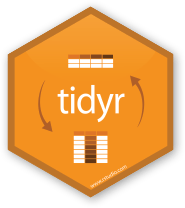
\includegraphics{tidyr.png}

Given a two dimensional data structure, we can think of several ways we
might want to extract data. The first is to extract rows associated with
a certain feature. For example, if we had some basic data from an Army
Physical Fitness Test (APFT), we may want to extract rows based on
\texttt{SEX}, as seen below.

\begin{figure}[htbp]
\centering
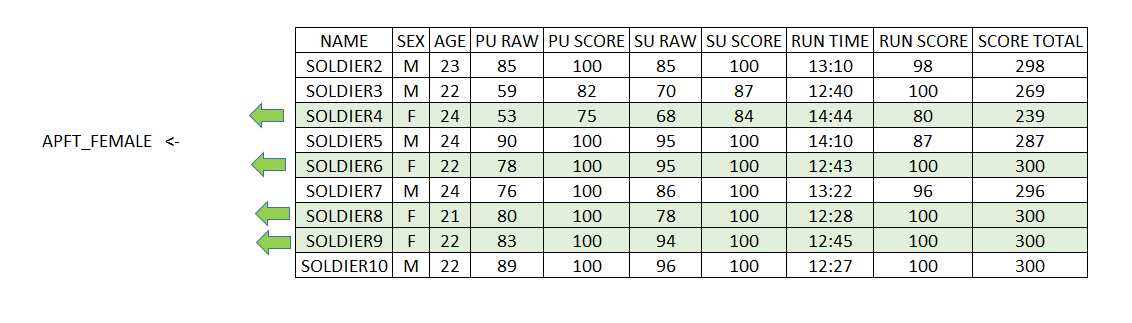
\includegraphics{filterRow.PNG}
\caption{Figure 2: Filtering Rows by Categorical Variable}
\end{figure}

We can conduct this same operation (extract all FEMALE records) on our
\texttt{kor} data frame with the \texttt{dplyr} package using the
following command:

\begin{Shaded}
\begin{Highlighting}[]
\KeywordTok{library}\NormalTok{(dplyr)}
\NormalTok{kor_female <-}\StringTok{ }\NormalTok{dplyr::}\KeywordTok{filter}\NormalTok{(kor, SEX==}\StringTok{"F"}\NormalTok{)}
\end{Highlighting}
\end{Shaded}

This command should produce a new data frame in your environment that
has has two rows and 25 columns. This new data frame only contains the
two FEMALE casualties represented in the data. To explore this much
smaller data set, we could now table the data frame based on state:

\begin{Shaded}
\begin{Highlighting}[]
\KeywordTok{table}\NormalTok{(kor_female$HOME_STATE)}
\end{Highlighting}
\end{Shaded}

\begin{verbatim}
## 
##          IOWA WEST VIRGINIA 
##             1             1
\end{verbatim}

We find out that one woman is from Iowa, and the other is from West
Virginia. If we table based on rank:

\begin{Shaded}
\begin{Highlighting}[]
\KeywordTok{table}\NormalTok{(kor_female$RANK)}
\end{Highlighting}
\end{Shaded}

\begin{verbatim}
## 
## 1STLT 
##     2
\end{verbatim}

We now know that both women were junior officers. If you take a look at
the data further, you will learn that both women were in the Air Force
and died in a non-hostile accident in 1952 on the same day (presumably
the same accident).

Note that we can also filter rows based on a Boolean function. For
example, if we wanted to only look at casualties that were over 30 years
old in 1950, we could filter with the following \texttt{dplyr} command:

\begin{Shaded}
\begin{Highlighting}[]
\NormalTok{kor_Over30 <-}\StringTok{ }\KeywordTok{filter}\NormalTok{(kor, BIRTH_YEAR <}\StringTok{ }\DecValTok{1920}\NormalTok{)  }\CommentTok{# Filter those older than 30 in 1950}
\end{Highlighting}
\end{Shaded}

When you run this command, you will find that our cleaned data produces
2220 records of casualties who were over 30 in the year 1950. If we want
to only select those individuals that were in their 30s in 1950, we
would use the following \texttt{dplyr} command:

\begin{Shaded}
\begin{Highlighting}[]
\NormalTok{kor_30s <-}\StringTok{ }\KeywordTok{filter}\NormalTok{(kor, BIRTH_YEAR <}\StringTok{ }\DecValTok{1920} \NormalTok{&}\StringTok{ }\NormalTok{BIRTH_YEAR >=}\StringTok{ }\DecValTok{1910}\NormalTok{)}
\end{Highlighting}
\end{Shaded}

Running this command shows that 2,052 of the casualties were in their
30s in 1950.

Now that we've filtered by row, let's filter by column. We've already
demonstrated above how to do this with the bracket notation. Now we will
illustrate how to do this using the \texttt{dplyr} package. We often
find that we've loaded data that has many columns that are not of
interest. In these cases, it is often helpful to extract only the
columns that we're interested in. This will also shrink the size of our
data in memory and make our code run faster. In the picture below, we
illustrate this with some simple APFT data. In this case we're
extracting the demographic and raw score columns:

\begin{figure}[htbp]
\centering
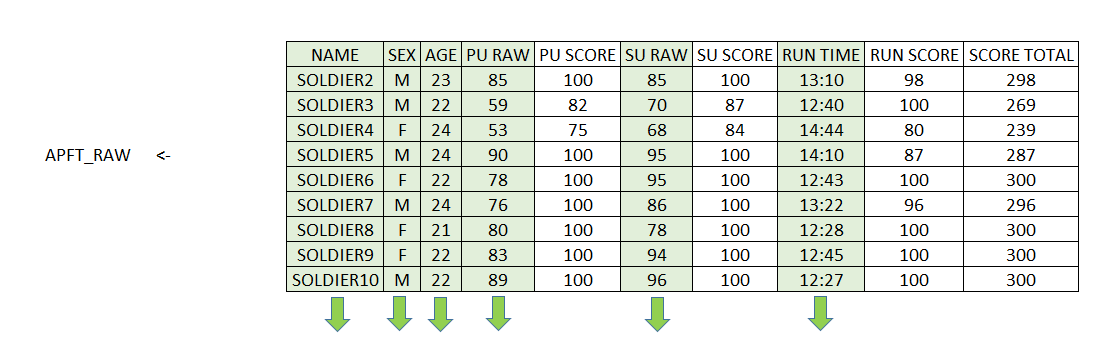
\includegraphics{filterColumn.PNG}
\caption{Figure 3: Filtering Specific Columns (or fields)}
\end{figure}

Let's say we are studying the Korean Casualty data to understand the
time factor of those who died of wounds, and we are particularly
interested in the time between \texttt{INCIDENT\_DATE} and
\texttt{FATALITY\_DATE}. Below we'll extract these two columns with the
\texttt{dplyr} package:

\begin{Shaded}
\begin{Highlighting}[]
\NormalTok{kor_dates <-}\StringTok{ }\KeywordTok{select}\NormalTok{(kor, }\KeywordTok{one_of}\NormalTok{(}\KeywordTok{c}\NormalTok{(}\StringTok{"INCIDENT_DATE"}\NormalTok{,}\StringTok{"FATALITY_DATE"}\NormalTok{))) }\CommentTok{#Select two columns}
\end{Highlighting}
\end{Shaded}

Now let's look at the structure of this new data frame:

\begin{Shaded}
\begin{Highlighting}[]
\KeywordTok{str}\NormalTok{(kor_dates)}
\end{Highlighting}
\end{Shaded}

\begin{verbatim}
## 'data.frame':    33899 obs. of  2 variables:
##  $ INCIDENT_DATE: chr  "19510412" "19500727" "19510316" "19530122" ...
##  $ FATALITY_DATE: chr  "20010402" "19500727" "19510316" "19530122" ...
\end{verbatim}

We see that we only have two columns, but we still have all 33,899 rows.
The code below is beyond the extent of this lesson on filtering (it
contains some code we'll go over in Lesson 5), but is interesting to
look at the difference between incident date and fatality date. In this
code we will load the \texttt{lubridate} package \citep{R-lubridate} and
use it to convert these two columns to date format and calculate the
difference between them (i.e., the number of days between the incident
and the death of the Service Member).

\begin{Shaded}
\begin{Highlighting}[]
\KeywordTok{library}\NormalTok{(lubridate)}
\NormalTok{days <-}\StringTok{ }\KeywordTok{ymd}\NormalTok{(kor_dates$FATALITY_DATE) -}\StringTok{ }\KeywordTok{ymd}\NormalTok{(kor_dates$INCIDENT_DATE)}
\NormalTok{days[}\DecValTok{1}\NormalTok{:}\DecValTok{100}\NormalTok{]}
\end{Highlighting}
\end{Shaded}

\begin{verbatim}
## Time differences in days
##   [1] 18253     0     0     0     0     0     0     0     0     0 17697
##  [12]     0     0     0 18342    31     0     0     0  1153     0     3
##  [23]     0     0   355     0     0     0     0     0     0     0    53
##  [34]     0     0     0     0     0     0     0     0    NA     0     0
##  [45]    NA   469     0     0    NA     0     0   981     0     0     0
##  [56]     0     0  1131  1155    46     0     0     0     0     0    NA
##  [67]     0    NA     0  1125   959     0   469     0     0     0   969
##  [78]     0     0    31     0  1130     0     0     0 17568     0  1155
##  [89]   120     0   177     0   154     0     0     7     0     0    NA
## [100]     0
\end{verbatim}

Looking at the first few entries should raise some questions. The very
first entry had 18,253 days between the incident and the fatality. In
fact, if you look closer at the dates, you will see that this Service
Member had an incident on 12 April 1951, but wasn't considered a
fatality until 2 April 2001. Let's plot a histogram of the difference in
days (you'll learn this command during the next lesson):

\begin{Shaded}
\begin{Highlighting}[]
\CommentTok{#plot histogram of difference in days}
\KeywordTok{hist}\NormalTok{(}\KeywordTok{as.numeric}\NormalTok{(days), }\DataTypeTok{main=}\StringTok{"Histogram of Difference in Days"}\NormalTok{, }\DataTypeTok{xlab=}\StringTok{"Days"}\NormalTok{)  }
\end{Highlighting}
\end{Shaded}

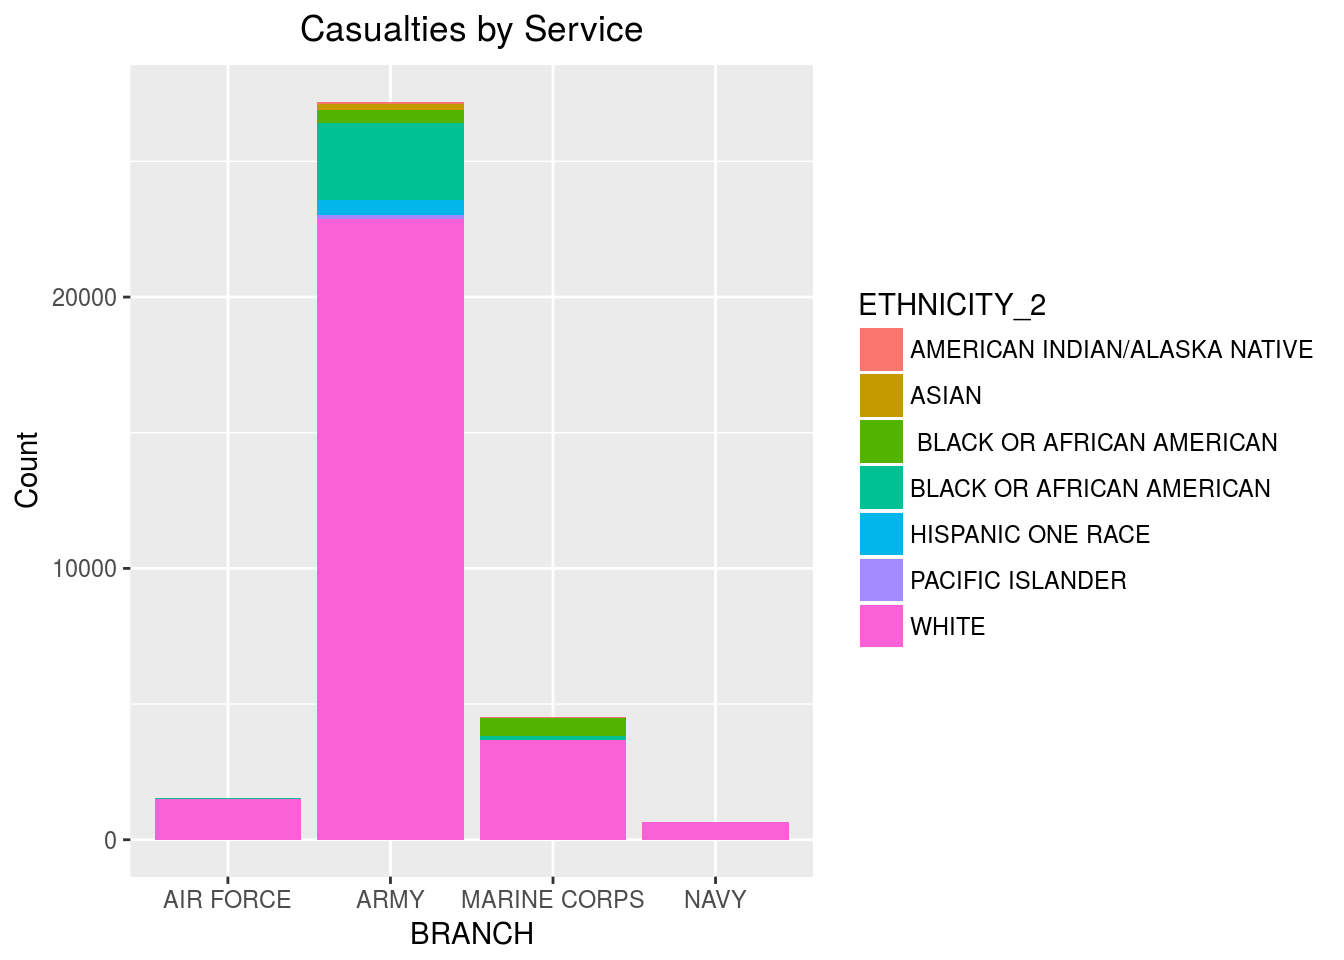
\includegraphics{bookdown-demo_files/figure-latex/unnamed-chunk-66-1.pdf}

Here we see that there are many casualties that have a fatality day
around the year 2000. If you look at the original data, you will see
that the first Service Member in the data (an Air Force Captain) is
listed with an incident year of 1951 and \texttt{FATALITY\_DATE} in
2001. Notice that the FATALITY status is \emph{DECLARED DEAD}. This
officer, as part of a bombing group, must have had MIA status for
several decades until finally ``declared dead'' in 2001. The ``declared
dead'' date became his fatality date, which means it would be difficult
to evaluate the temporal aspect of wound care without addressing the
presence of lengthy MIA periods in the data.

\section{Using the grep and aggregate
commands}\label{using-the-grep-and-aggregate-commands}

The following video illustrates how to use the \texttt{grep()} and
\texttt{aggregate()} commands. This video will use a new APFT data set.

\begin{Shaded}
\begin{Highlighting}[]
\KeywordTok{download.file}\NormalTok{(}\StringTok{"https://s3.amazonaws.com/dscoe-data-2/apft.csv"}\NormalTok{, }\DataTypeTok{destfile =} \StringTok{"apft.csv"}\NormalTok{)}
\end{Highlighting}
\end{Shaded}

\section{Summary}\label{summary}

What we have seen is that R provides a great platform to rapidly
``wrangle'' and explore data. Exploring a data set allows you to find
items of interest as well as any limitations that may be not be obvious
at first. There is no perfect approach to do this exploration of a data
set, but there is great value in learning the commands necessary to
follow your curiosity and intuition.

\section{Practice Problem}\label{practice-problem-1}

\begin{enumerate}
\def\labelenumi{\arabic{enumi}.}
\tightlist
\item
  Use grep to determine how many casualties had \emph{INFANTRY}
  somewhere in the title (use the \texttt{POSITION} field).
\end{enumerate}

\chapter{Basic Visualization}\label{basic-visualization}

The R programming language has some of the most powerful data
visualization packages available. These packages are continually
expanded upon, and new data visualization packages are created on a
regular basis. In addition to packages that create basic statistical
visualization (line plots, bar plots, pie charts, etc.), there are
packages that create geospatial visualizations, 3D visualizations, and
interactive visualizations.

Let's start by reading in the Korean Conflict data and performing the
primary cleaning functions that we performed last lesson.

\begin{Shaded}
\begin{Highlighting}[]
\NormalTok{kor <-}\StringTok{ }\KeywordTok{read.csv}\NormalTok{(}\StringTok{'KoreanConflict.csv'}\NormalTok{, }\DataTypeTok{as.is=}\OtherTok{TRUE}\NormalTok{)}
\NormalTok{kor$BIRTH_YEAR <-}\StringTok{ }\KeywordTok{as.numeric}\NormalTok{(kor$BIRTH_YEAR)}
\NormalTok{kor <-}\StringTok{ }\NormalTok{kor[!}\KeywordTok{is.na}\NormalTok{(kor$BIRTH_YEAR),]}
\end{Highlighting}
\end{Shaded}

Now that we have the data in memory, we will use some basic
visualizations to explore the data. In this lesson, we will primarily
use visualizations from the ggplot2 package \citep{R-ggplot2}. If you
haven't installed this package before, run the command
\texttt{install.packages(\textquotesingle{}ggplot2\textquotesingle{})}.

\section{Bar Plot}\label{bar-plot}

We will start by producing a basic barplot of categorical variables.
First we'll look at the \texttt{BRANCH} field for the Korean Casualties.

\begin{Shaded}
\begin{Highlighting}[]
\KeywordTok{library}\NormalTok{(ggplot2)}
\KeywordTok{ggplot}\NormalTok{(kor, }\KeywordTok{aes}\NormalTok{(BRANCH)) +}\StringTok{ }\KeywordTok{geom_bar}\NormalTok{()}
\end{Highlighting}
\end{Shaded}

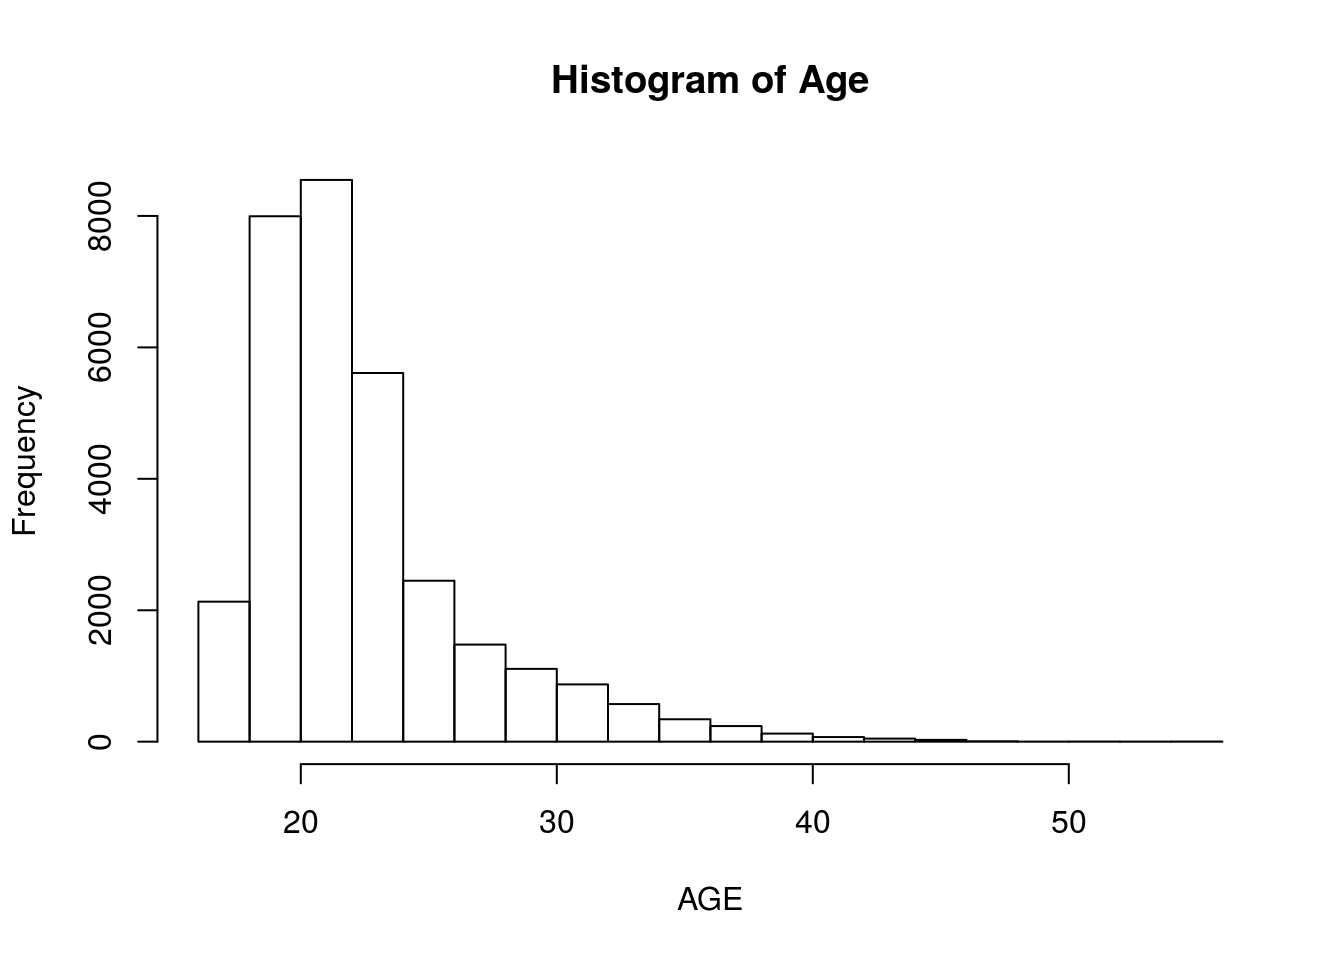
\includegraphics{bookdown-demo_files/figure-latex/unnamed-chunk-69-1.pdf}

Let's break down what this command is actually doing. The
\texttt{ggplot} command is the start of any \texttt{ggplot2}
visualization. In this \texttt{ggplot()} command, we say that we want a
visualization of the \texttt{kor} data set with a focus on the
\texttt{BRANCH} variable, referred to as the \emph{aesthetic} (aes) in
the \texttt{ggplot2} package. The next command says to take the data
we've identified (\texttt{BRANCH} variable from the \texttt{kor} data
frame) and create a barplot (\texttt{geom\_} specifies the geometry or
shape/style of plot we want).

We can uniquely color the bars by adding \texttt{fill\ =\ BRANCH} to
specify that each bar's fill color should be associated with the
\texttt{BRANCH}.

\begin{Shaded}
\begin{Highlighting}[]
\KeywordTok{ggplot}\NormalTok{(kor, }\KeywordTok{aes}\NormalTok{(BRANCH, }\DataTypeTok{fill =} \NormalTok{BRANCH)) +}\StringTok{ }\KeywordTok{geom_bar}\NormalTok{()}
\end{Highlighting}
\end{Shaded}

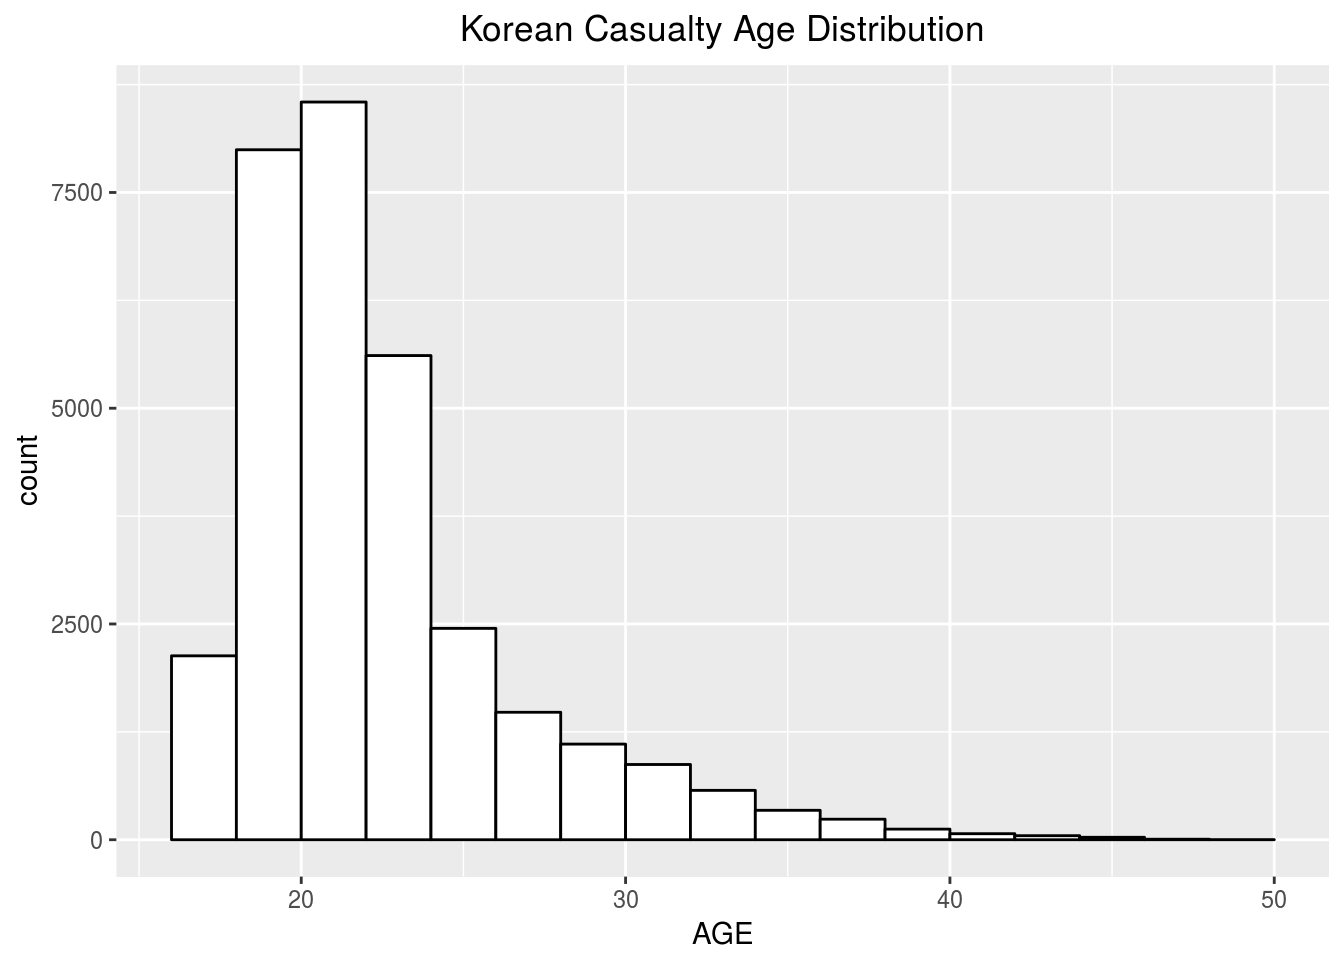
\includegraphics{bookdown-demo_files/figure-latex/unnamed-chunk-70-1.pdf}

We may also want to add a title and get rid of the legend since the
labels are already on the horizontal axis.

\begin{Shaded}
\begin{Highlighting}[]
\KeywordTok{ggplot}\NormalTok{(kor, }\KeywordTok{aes}\NormalTok{(BRANCH, }\DataTypeTok{fill =} \NormalTok{BRANCH)) +}\StringTok{ }\KeywordTok{geom_bar}\NormalTok{() +}\StringTok{ }
\StringTok{  }\KeywordTok{ggtitle}\NormalTok{(}\StringTok{"Casualties by Service"}\NormalTok{) +}\StringTok{ }\KeywordTok{theme}\NormalTok{(}\DataTypeTok{legend.position=}\StringTok{"none"}\NormalTok{)}
\end{Highlighting}
\end{Shaded}

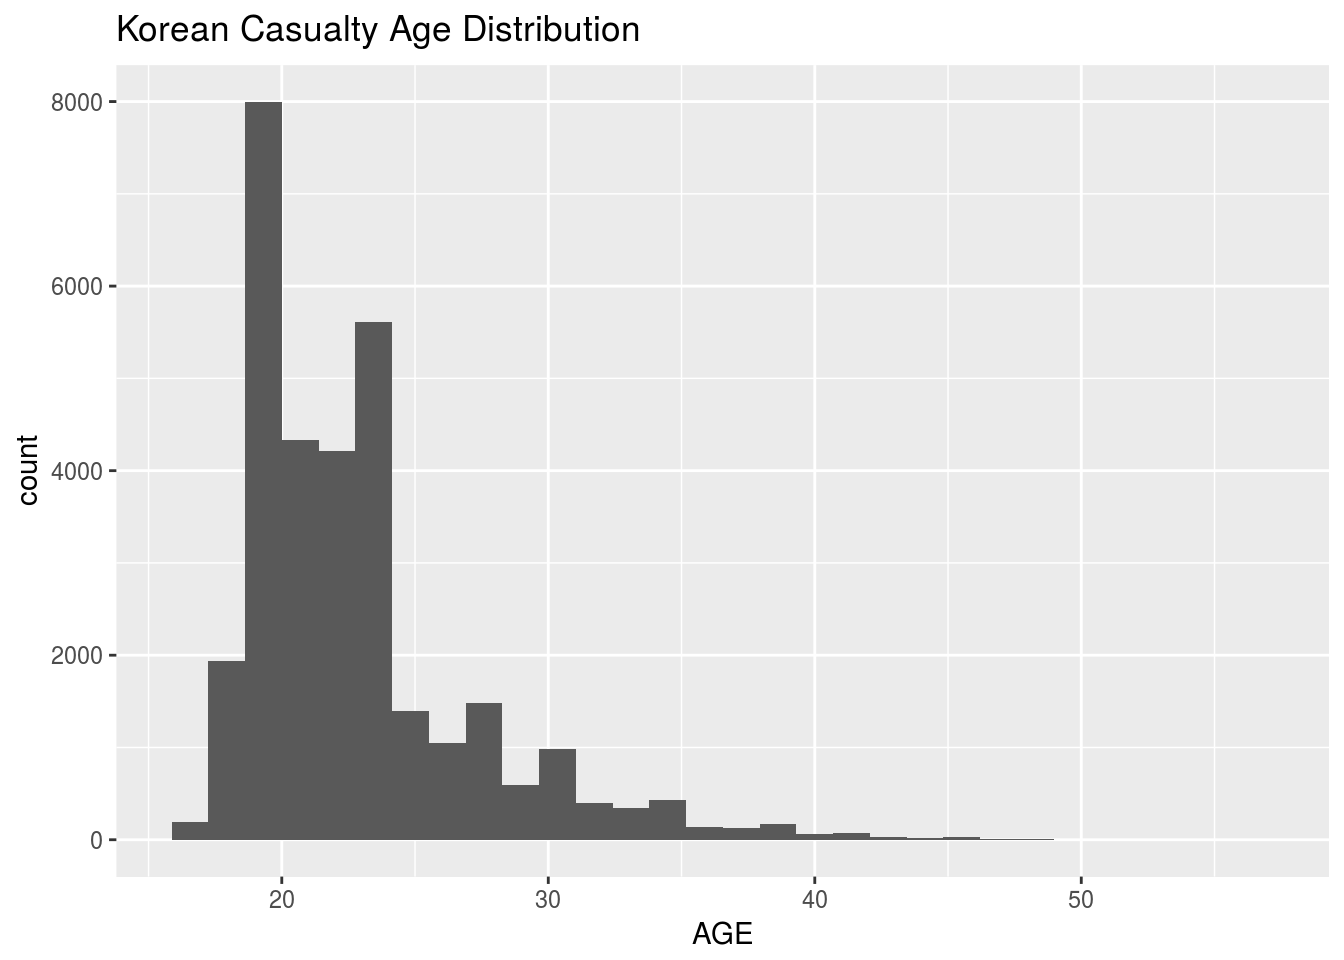
\includegraphics{bookdown-demo_files/figure-latex/unnamed-chunk-71-1.pdf}

This plot is starting to look pretty nice, but centering the title and
capitalizing the vertical axis label would be good finishing touches.
While the code below may look complicated, a quick internet search will
produce a ``how-to'' for just about any plot modification you can
imagine. As an example, perform a Google search for ``center a ggtitle''
(you should find the solution below in the first linked search result).

\begin{Shaded}
\begin{Highlighting}[]
\KeywordTok{ggplot}\NormalTok{(kor, }\KeywordTok{aes}\NormalTok{(BRANCH, }\DataTypeTok{fill =} \NormalTok{BRANCH)) +}\StringTok{ }\KeywordTok{geom_bar}\NormalTok{() +}\StringTok{ }
\StringTok{  }\KeywordTok{ggtitle}\NormalTok{(}\StringTok{"Casualties by Service"}\NormalTok{) +}\StringTok{ }
\StringTok{  }\KeywordTok{theme}\NormalTok{(}\DataTypeTok{plot.title =} \KeywordTok{element_text}\NormalTok{(}\DataTypeTok{hjust =} \FloatTok{0.5}\NormalTok{)) +}\StringTok{ }
\StringTok{  }\KeywordTok{ylab}\NormalTok{(}\StringTok{"Count"}\NormalTok{) +}\StringTok{ }\KeywordTok{theme}\NormalTok{(}\DataTypeTok{legend.position=}\StringTok{"none"}\NormalTok{)}
\end{Highlighting}
\end{Shaded}

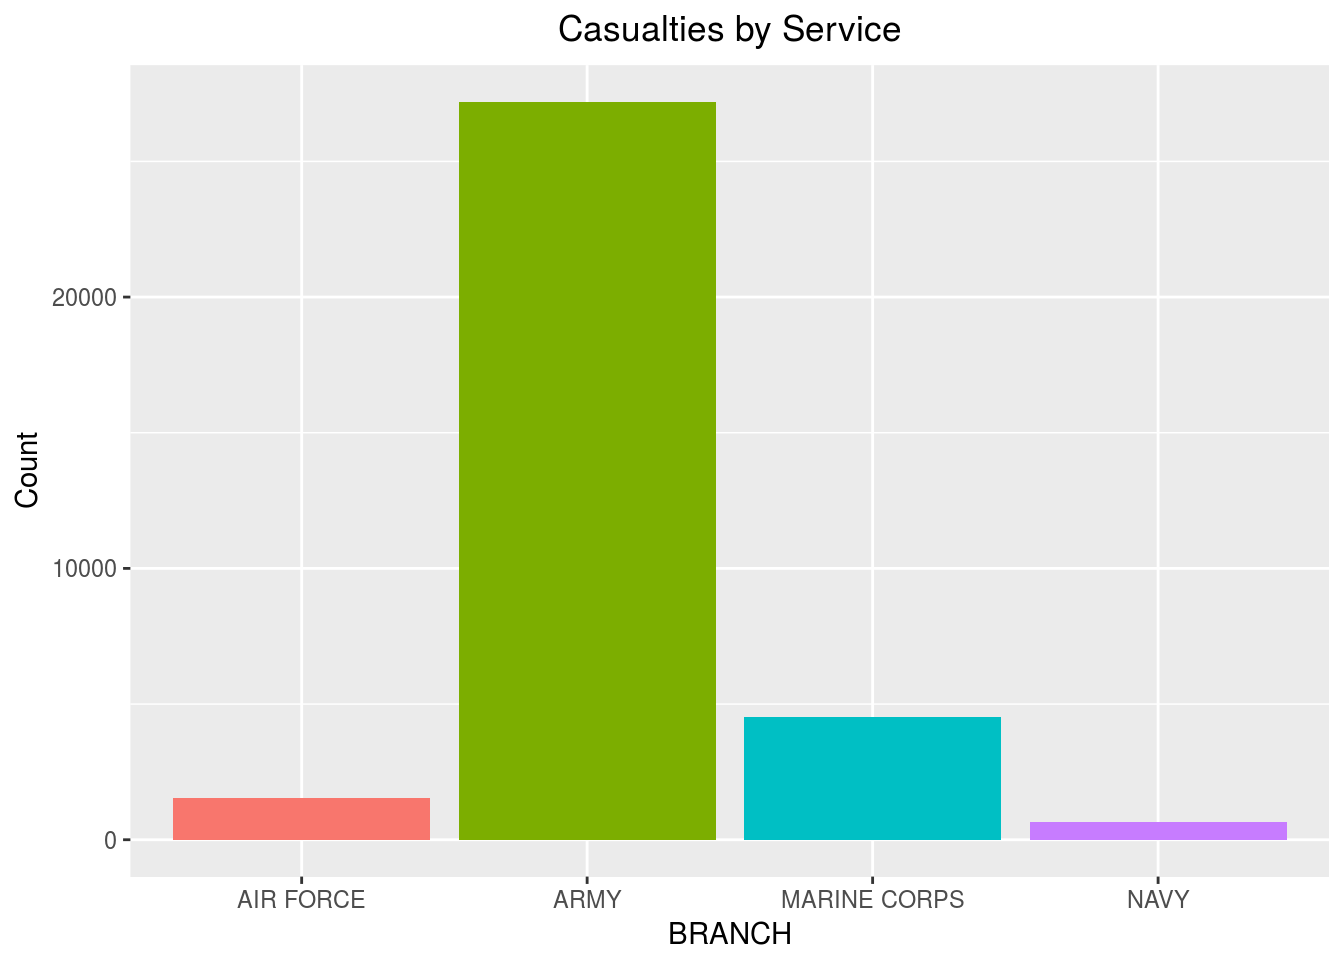
\includegraphics{bookdown-demo_files/figure-latex/unnamed-chunk-72-1.pdf}

As we continued adding more and more pieces to our plot command, you'll
notice each piece was simply connected with the \texttt{+} operator. The
``gg'' in \texttt{ggplot()} stands for ``grammar of graphics,'' and you
can think about each component of our plot command being an aspect of a
sentence. We first defined the subject when we specified \texttt{kor}
and \texttt{BRANCH}. We added the ``what'' and ``how'' when we
instructed R to build a certain type of plot in a certain way. Think
about this ``grammar of graphics'' structure as we continue to build
more and more complex and tailorable visualizations.

Now let's build a stacked barplot. Say we wanted to see the distribution
of \texttt{ETHNICITY} in each of the service \texttt{BRANCHES}. First,
let's take a look at our categories:

\begin{Shaded}
\begin{Highlighting}[]
\KeywordTok{table}\NormalTok{(kor$ETHNICITY_2)}
\end{Highlighting}
\end{Shaded}

\begin{verbatim}
## 
##             AMERICAN INDIAN/ALASKA NATIVE 
##                                       103 
##                                     ASIAN 
##                                       229 
##                 BLACK OR AFRICAN AMERICAN 
##                                      1146 
##                 BLACK OR AFRICAN AMERICAN 
##                                      3022 
##                         HISPANIC ONE RACE 
##                                       566 
## NATIVE HAWAIIAN OR OTHER PACIFIC ISLANDER 
##                                       142 
##                                     WHITE 
##                                     28691
\end{verbatim}

These are rather long names to display on a chart. We will start by
creating shorter names. We can do this in the code below using the
\texttt{grep()} command that we learned in Lesson 2. We can replace
``Native Hawaiian or other Pacific Islander'' with simply ``Pacific
Islander'' as follows:

\begin{Shaded}
\begin{Highlighting}[]
\NormalTok{kor$ETHNICITY_2[}\KeywordTok{grep}\NormalTok{(}\StringTok{"HAWAIIAN"}\NormalTok{,kor$ETHNICITY_2)] <-}\StringTok{ "PACIFIC ISLANDER"}
\end{Highlighting}
\end{Shaded}

Now all we have to do in our previous code is change the
\texttt{fill\ =\ BRANCH} to \texttt{fill\ =\ ETHNICITY\_2}. We also
don't want to discard the legend anymore.

\begin{Shaded}
\begin{Highlighting}[]
\KeywordTok{ggplot}\NormalTok{(kor, }\KeywordTok{aes}\NormalTok{(BRANCH, }\DataTypeTok{fill =} \NormalTok{ETHNICITY_2)) +}\StringTok{ }\KeywordTok{geom_bar}\NormalTok{() +}\StringTok{ }
\StringTok{  }\KeywordTok{ggtitle}\NormalTok{(}\StringTok{"Casualties by Service and Ethnicity"}\NormalTok{) +}\StringTok{ }
\StringTok{  }\KeywordTok{theme}\NormalTok{(}\DataTypeTok{plot.title =} \KeywordTok{element_text}\NormalTok{(}\DataTypeTok{hjust =} \FloatTok{0.5}\NormalTok{)) +}\StringTok{ }\KeywordTok{ylab}\NormalTok{(}\StringTok{"Count"}\NormalTok{)}
\end{Highlighting}
\end{Shaded}

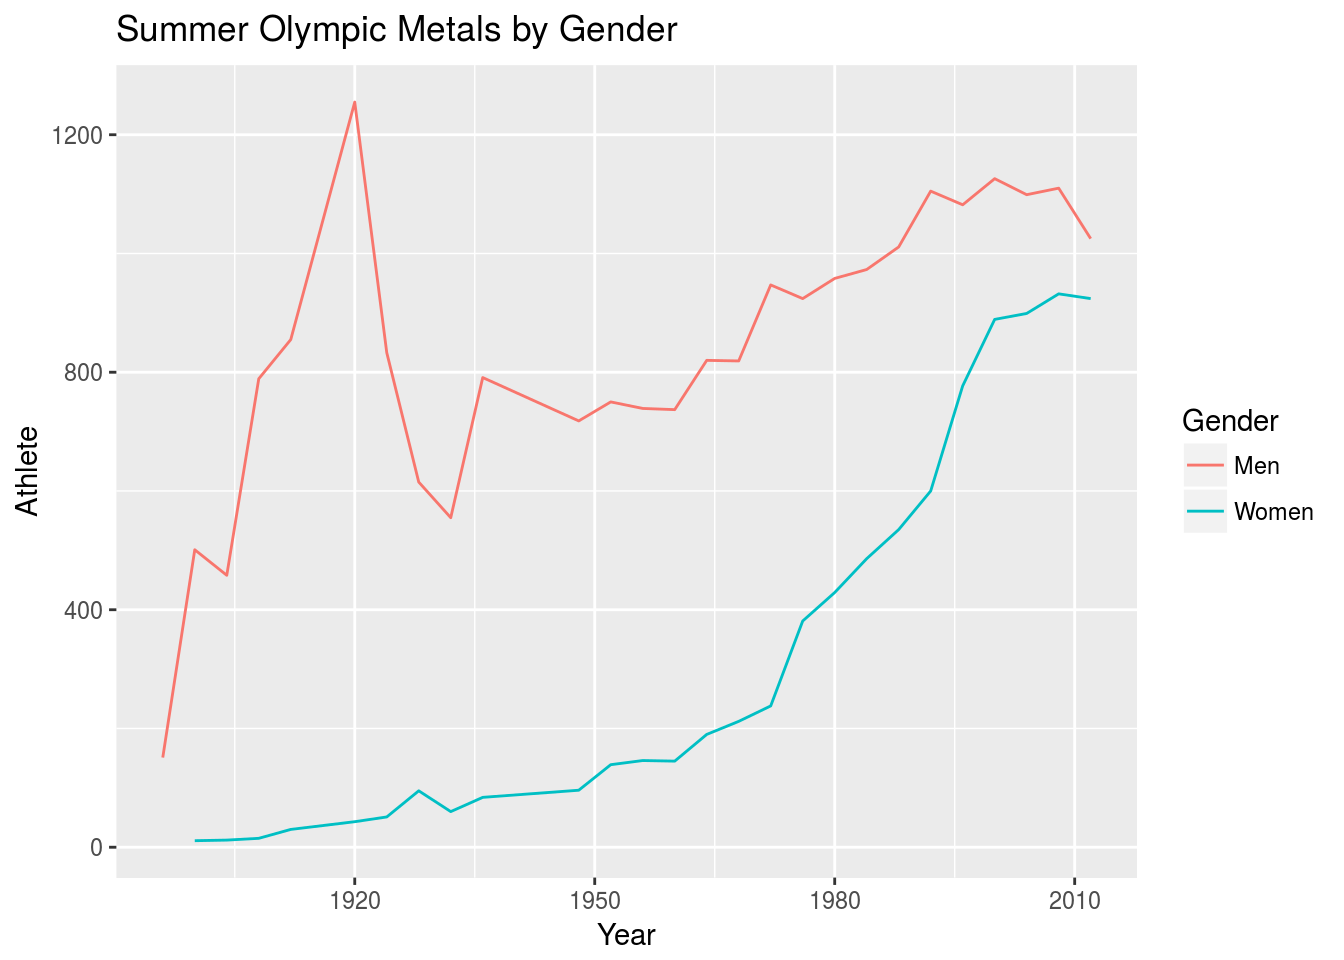
\includegraphics{bookdown-demo_files/figure-latex/unnamed-chunk-75-1.pdf}

\section{Pie Chart}\label{pie-chart}

Statisticians will generally tell you that you should never use a pie
chart. Usually a bar plot is recommended because it is easier for the
human eye to distinguish differences in magnitude. That being said,
there are still a few times when a pie chart is necessary. For this
plot, we are going to use a function from the BASE graphics package
(this comes with R, and you don't have to load it). The pie chart is
very easy to produce if we wrap the \texttt{pie()} command around the
\texttt{table} command:

\begin{Shaded}
\begin{Highlighting}[]
\KeywordTok{pie}\NormalTok{(}\KeywordTok{table}\NormalTok{(kor$BRANCH), }\DataTypeTok{main =} \StringTok{"Korean War Casualties by Service"}\NormalTok{)}
\end{Highlighting}
\end{Shaded}

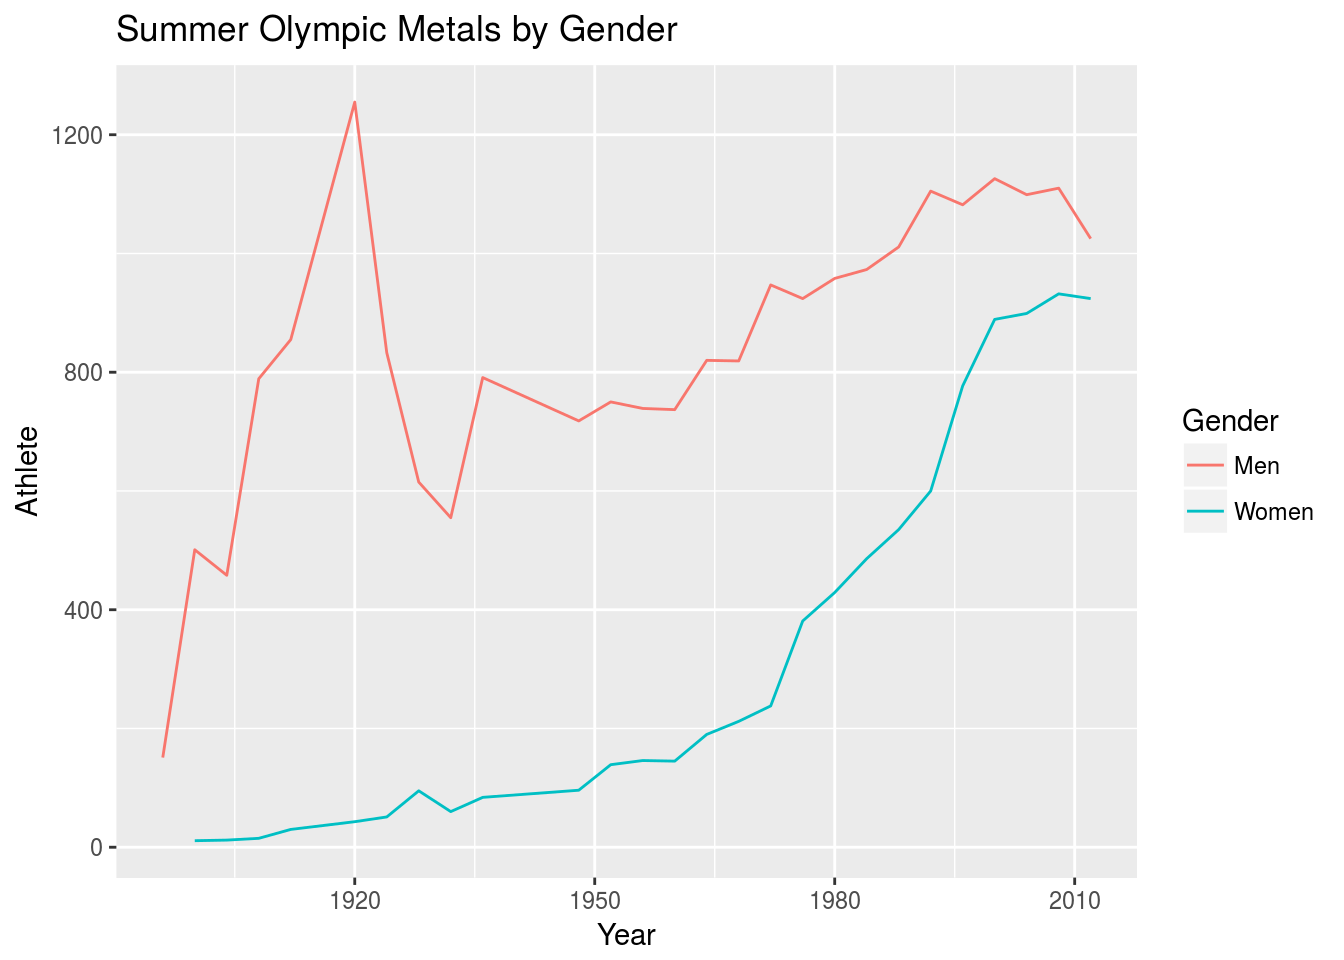
\includegraphics{bookdown-demo_files/figure-latex/unnamed-chunk-76-1.pdf}

\section{Histogram Plot}\label{histogram-plot}

Now we'll take a look at several ways to create \emph{histograms} in R.
This is where R will quickly outshine Microsoft Excel and other
spreadsheet programs. While Excel can create a barplot just like R, it
is extremely time consuming to create a \emph{histogram} in Excel. R
will create a histogram in one line of code.

Let's create a histogram of the age for each Korean Conflict casualty.
Notice that we don't have a field that has \emph{age} in it, but we do
have the \texttt{BIRTH\_YEAR} and \texttt{FATALITY\_YEAR}. The
calculation below will create a new field that is the \texttt{AGE} of
the casualty at death (notice that we remove all records with a
\texttt{FATALITY\_DATE} after 1960 in order to remove those who were MIA
and declared dead at a later time).

\begin{Shaded}
\begin{Highlighting}[]
\CommentTok{# Filter our MIA}
\NormalTok{kor2 <-}\StringTok{ }\NormalTok{dplyr::}\KeywordTok{filter}\NormalTok{(kor, FATALITY_DATE <}\StringTok{ }\DecValTok{1960}\NormalTok{) }

\CommentTok{# Coerce to numeric}
\NormalTok{kor2$FATALITY_YEAR <-}\StringTok{ }\KeywordTok{as.numeric}\NormalTok{(kor2$FATALITY_YEAR)  }
\NormalTok{kor2$BIRTH_YEAR <-}\StringTok{ }\KeywordTok{as.numeric}\NormalTok{(kor2$BIRTH_YEAR)}

\CommentTok{# Create AGE field}
\NormalTok{kor2$AGE <-}\StringTok{ }\NormalTok{kor2$FATALITY_YEAR -}\StringTok{ }\NormalTok{kor2$BIRTH_YEAR      }
\end{Highlighting}
\end{Shaded}

Now that we've created the \texttt{AGE} field, we will use two different
techniques to create a histogram. The Base R package has a histogram
function that is easy to use and helpful for exploring data.

\begin{Shaded}
\begin{Highlighting}[]
\KeywordTok{hist}\NormalTok{(kor2$AGE, }\DataTypeTok{freq=}\OtherTok{TRUE}\NormalTok{, }\DataTypeTok{main =} \StringTok{"Korean Conflict Casualty Age Distribution"}\NormalTok{, }\DataTypeTok{xlab =} \StringTok{"AGE"}\NormalTok{)}
\end{Highlighting}
\end{Shaded}

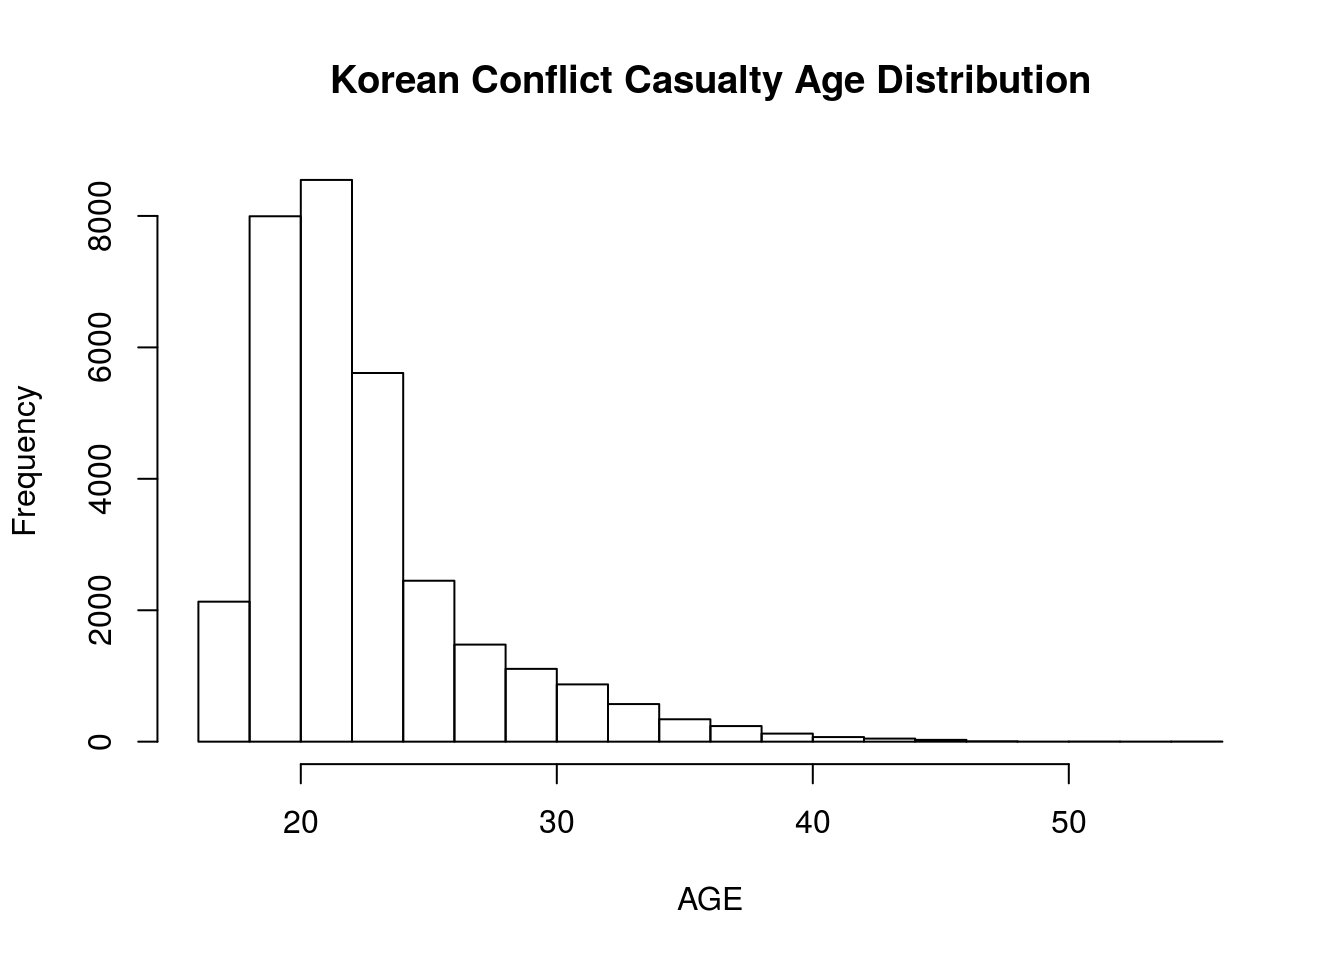
\includegraphics{bookdown-demo_files/figure-latex/unnamed-chunk-78-1.pdf}

The \texttt{ggplot2} package also has the ability to generate a
histogram that is generally better for presentations.

\begin{Shaded}
\begin{Highlighting}[]
\KeywordTok{ggplot}\NormalTok{(kor2, }\KeywordTok{aes}\NormalTok{(AGE)) +}\StringTok{ }
\StringTok{  }\KeywordTok{geom_histogram}\NormalTok{(}\DataTypeTok{breaks=}\KeywordTok{seq}\NormalTok{(}\DecValTok{16}\NormalTok{,}\DecValTok{50}\NormalTok{, }\DataTypeTok{by=}\DecValTok{2}\NormalTok{), }\DataTypeTok{col=}\StringTok{"black"}\NormalTok{, }\DataTypeTok{fill=}\StringTok{"white"}\NormalTok{) +}\StringTok{ }
\StringTok{  }\KeywordTok{ggtitle}\NormalTok{(}\StringTok{'Korean Conflict Casualty Age Distribution'}\NormalTok{) +}\StringTok{ }
\StringTok{  }\KeywordTok{theme}\NormalTok{(}\DataTypeTok{plot.title =} \KeywordTok{element_text}\NormalTok{(}\DataTypeTok{hjust =} \FloatTok{0.5}\NormalTok{))}
\end{Highlighting}
\end{Shaded}

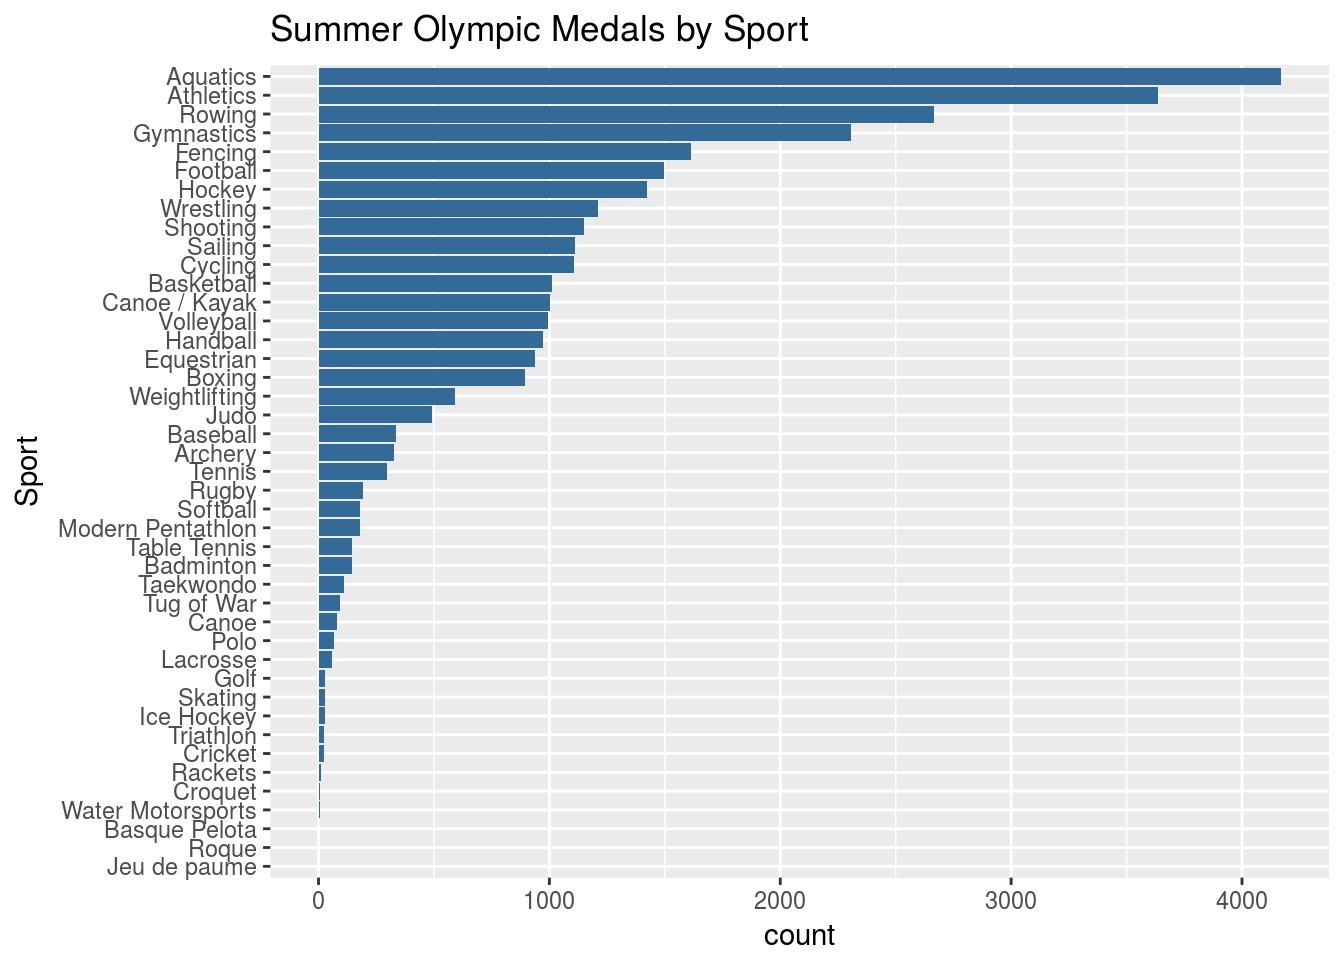
\includegraphics{bookdown-demo_files/figure-latex/unnamed-chunk-79-1.pdf}

\section{Time Series Plot}\label{time-series-plot}

Time series plots (and line plots in general) are helpful in visually
identifying trends and anomalies in data. We are going to change our
data sets now to look at the Olympic medal counts. This data set lists
all Olympic medals won during a Summer Olympics from 1896 to 2012. This
data set is available here:

\url{https://s3.amazonaws.com/dscoe-data-2/summer.csv}

You can download the file with the following command:

\begin{Shaded}
\begin{Highlighting}[]
\KeywordTok{download.file}\NormalTok{(}\StringTok{"https://s3.amazonaws.com/dscoe-data-2/summer.csv"}\NormalTok{, }
              \DataTypeTok{destfile =} \StringTok{"summer.csv"}\NormalTok{)}
\end{Highlighting}
\end{Shaded}

Now that you've acquired the data, read it into R and take a look at its
structure with the following two commands:

\begin{Shaded}
\begin{Highlighting}[]
\NormalTok{oly <-}\StringTok{ }\KeywordTok{read.csv}\NormalTok{(}\StringTok{'summer.csv'}\NormalTok{, }\DataTypeTok{as.is =} \OtherTok{TRUE}\NormalTok{)}
\KeywordTok{str}\NormalTok{(oly)}
\end{Highlighting}
\end{Shaded}

\begin{verbatim}
## 'data.frame':    31165 obs. of  9 variables:
##  $ Year      : int  1896 1896 1896 1896 1896 1896 1896 1896 1896 1896 ...
##  $ City      : chr  "Athens" "Athens" "Athens" "Athens" ...
##  $ Sport     : chr  "Aquatics" "Aquatics" "Aquatics" "Aquatics" ...
##  $ Discipline: chr  "Swimming" "Swimming" "Swimming" "Swimming" ...
##  $ Athlete   : chr  "HAJOS, Alfred" "HERSCHMANN, Otto" "DRIVAS, Dimitrios" "MALOKINIS, Ioannis" ...
##  $ Country   : chr  "HUN" "AUT" "GRE" "GRE" ...
##  $ Gender    : chr  "Men" "Men" "Men" "Men" ...
##  $ Event     : chr  "100M Freestyle" "100M Freestyle" "100M Freestyle For Sailors" "100M Freestyle For Sailors" ...
##  $ Medal     : chr  "Gold" "Silver" "Bronze" "Gold" ...
\end{verbatim}

Let's say that we want to explore the trend of increased numbers of
women participating in the Summer Olympics over the past century. The
\texttt{dplyr} package offers an \texttt{aggregate()} function that will
help us do this. Let's start by aggregating the number of Olympic medals
by \texttt{Year} and \texttt{Gender}:

\begin{Shaded}
\begin{Highlighting}[]
\CommentTok{# Take the full list of athletes, split it up into many sublists }
\CommentTok{# by year and by gender, and return the length of each sublist.}
\NormalTok{oly_sum <-}\StringTok{ }\KeywordTok{aggregate}\NormalTok{(Athlete ~}\StringTok{ }\NormalTok{Year +}\StringTok{ }\NormalTok{Gender, }\DataTypeTok{data=}\NormalTok{oly, length)}
\end{Highlighting}
\end{Shaded}

Let's take a look at the first few and last few lines of this new data
set to make sure that it aggregated the data as we anticipated:

\begin{Shaded}
\begin{Highlighting}[]
\KeywordTok{head}\NormalTok{(oly_sum)}
\end{Highlighting}
\end{Shaded}

\begin{verbatim}
##   Year Gender Athlete
## 1 1896    Men     151
## 2 1900    Men     501
## 3 1904    Men     458
## 4 1908    Men     789
## 5 1912    Men     855
## 6 1920    Men    1255
\end{verbatim}

\begin{Shaded}
\begin{Highlighting}[]
\KeywordTok{tail}\NormalTok{(oly_sum)}
\end{Highlighting}
\end{Shaded}

\begin{verbatim}
##    Year Gender Athlete
## 48 1992  Women     600
## 49 1996  Women     777
## 50 2000  Women     889
## 51 2004  Women     899
## 52 2008  Women     932
## 53 2012  Women     924
\end{verbatim}

A final check for correctness requires us to sum the
\texttt{oly\_sum\$Athlete} counts. If the sum equals the total number of
athletes (31,165), that's a good sign.

\begin{Shaded}
\begin{Highlighting}[]
\KeywordTok{sum}\NormalTok{(oly_sum$Athlete)}
\end{Highlighting}
\end{Shaded}

\begin{verbatim}
## [1] 31165
\end{verbatim}

Everything looks good. Now we have a data set that we can use to create
a time series line plot. We create this plot below by specifying
\texttt{Year} as our horizontal or x-axis and \texttt{Athlete} as our
vertical or y-axis:

\begin{Shaded}
\begin{Highlighting}[]
\KeywordTok{ggplot}\NormalTok{(oly_sum, }\KeywordTok{aes}\NormalTok{(}\DataTypeTok{x=}\NormalTok{Year, }\DataTypeTok{y=}\NormalTok{Athlete, }\DataTypeTok{color =} \NormalTok{Gender)) +}\StringTok{ }
\StringTok{  }\KeywordTok{geom_line}\NormalTok{() +}\StringTok{ }\KeywordTok{ggtitle}\NormalTok{(}\StringTok{'Summer Olympic Medals by Gender'}\NormalTok{) +}\StringTok{ }
\StringTok{  }\KeywordTok{theme}\NormalTok{(}\DataTypeTok{plot.title =} \KeywordTok{element_text}\NormalTok{(}\DataTypeTok{hjust =} \FloatTok{0.5}\NormalTok{))}
\end{Highlighting}
\end{Shaded}

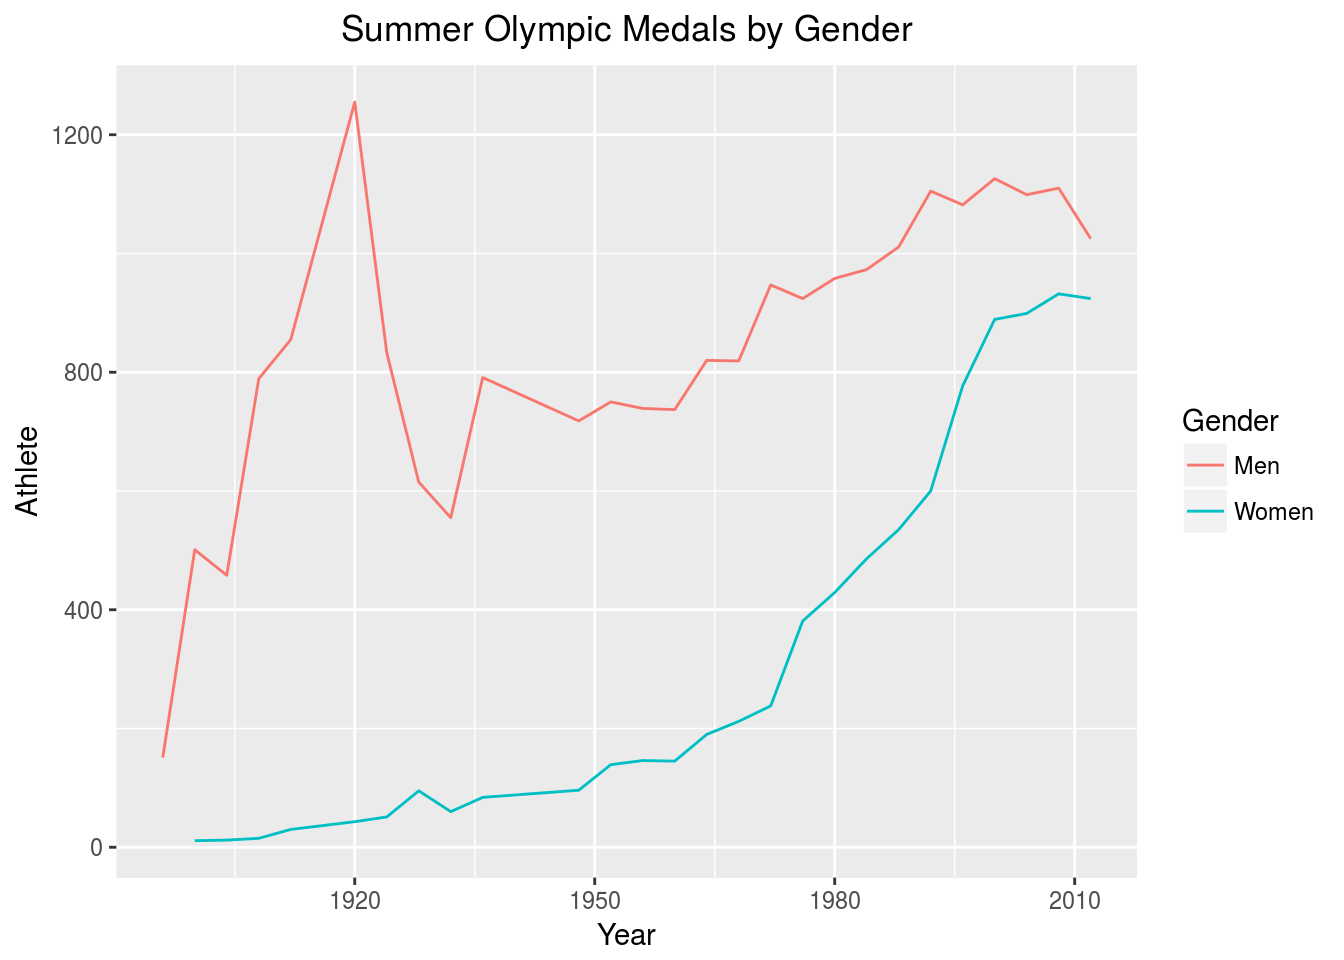
\includegraphics{bookdown-demo_files/figure-latex/unnamed-chunk-86-1.pdf}

From this graph we see that there was significant growth in the
participation of women in the Olympics starting in the 1970s. We also
see an interesting spike in the number of medals for men in the 1920s
that we could explore.

Now let's select a few of the prominent countries in the Summer
Olympics. Specifically, we'll look at the permanent members of the UN
Security Council: United States, Great Britain, France, China, and
Russia. Let's first look at the table of countries listed in the data
set.

\begin{Shaded}
\begin{Highlighting}[]
\KeywordTok{table}\NormalTok{(oly$Country)}
\end{Highlighting}
\end{Shaded}

\begin{verbatim}
## 
##       AFG  AHO  ALG  ANZ  ARG  ARM  AUS  AUT  AZE  BAH  BAR  BDI  BEL  BER 
##    4    2    1   15   29  259   11 1189  146   26   27    1    1  411    1 
##  BLR  BOH  BOT  BRA  BRN  BUL  BWI  CAN  CHI  CHN  CIV  CMR  COL  CRC  CRO 
##  113    7    1  431    1  333    5  649   33  807    1   23   19    4  114 
##  CUB  CYP  CZE  DEN  DJI  DOM  ECU  EGY  ERI  ESP  EST  ETH  EUA  EUN  FIN 
##  410    1   56  507    1    6    2   28    1  442   39   45  260  223  456 
##  FRA  FRG  GAB  GBR  GDR  GEO  GER  GHA  GRE  GRN  GUA  GUY  HAI  HKG  HUN 
## 1396  490    1 1720  825   25 1305   16  148    1    1    1    8    4 1079 
##  INA  IND  IOP  IRI  IRL  IRQ  ISL  ISR  ISV  ITA  JAM  JPN  KAZ  KEN  KGZ 
##   38  184    3   61   30    1   17    7    1 1296  127  788   49   93    3 
##  KOR  KSA  KUW  LAT  LIB  LTU  LUX  MAR  MAS  MDA  MEX  MGL  MKD  MNE  MOZ 
##  529    6    2   20    4   55    2   22    8    6  106   24    1   14    2 
##  MRI  NAM  NED  NGR  NIG  NOR  NZL  PAK  PAN  PAR  PER  PHI  POL  POR  PRK 
##    1    4  851   84    1  554  190  121    3   17   15    9  511   33   58 
##  PUR  QAT  ROU  RSA  RU1  RUS  SCG  SEN  SGP  SIN  SLO  SRB  SRI  SUD  SUI 
##    8    4  640  106   17  768   14    1    4    4   26   31    2    1  380 
##  SUR  SVK  SWE  SYR  TAN  TCH  TGA  THA  TJK  TOG  TPE  TRI  TTO  TUN  TUR 
##    2   34 1044    3    2  329    1   25    3    1   44   20   10   10   86 
##  UAE  UGA  UKR  URS  URU  USA  UZB  VEN  VIE  YUG  ZAM  ZIM  ZZX 
##    1    7  173 2049   76 4585   20   12    2  435    2   23   48
\end{verbatim}

Studying this data a bit, we see that the ISO-3 code for Russia changed
from \emph{URS} to \emph{RUS} after the fall of the Soviet Union. For
our analysis, we will change all \emph{URS} data to \emph{RUS}.

\begin{Shaded}
\begin{Highlighting}[]
\CommentTok{# Convert all URS medals to RUS medals.}
\NormalTok{oly$Country[oly$Country==}\StringTok{"URS"}\NormalTok{] <-}\StringTok{ "RUS"}
\end{Highlighting}
\end{Shaded}

Now will will aggregate the data by \texttt{Year} and \texttt{Country}
as well as reduce the country list to only those of interest. In the
code below, notice how we create a vector of our five countries and then
use the \texttt{\%in\%} function to filter out all countries not
contained in our list. In other words, we consider each medal winner and
retain that individual record only if his or her country is \emph{in}
our country list.

\begin{Shaded}
\begin{Highlighting}[]
\KeywordTok{library}\NormalTok{(dplyr)}
\CommentTok{# Aggregate all medals counts by country and year.}
\NormalTok{oly_country <-}\StringTok{ }\KeywordTok{aggregate}\NormalTok{(Medal ~}\StringTok{ }\NormalTok{Country +}\StringTok{ }\NormalTok{Year, }\DataTypeTok{data =} \NormalTok{oly, length)}
\NormalTok{country.list <-}\StringTok{ }\KeywordTok{c}\NormalTok{(}\StringTok{'USA'}\NormalTok{,}\StringTok{'GBR'}\NormalTok{,}\StringTok{'FRA'}\NormalTok{,}\StringTok{'CHN'}\NormalTok{,}\StringTok{'RUS'}\NormalTok{)}
\CommentTok{# Remove all counts associated with countries outside our list.}
\NormalTok{oly_country2 <-}\StringTok{ }\KeywordTok{filter}\NormalTok{(oly_country, Country %in%}\StringTok{ }\NormalTok{country.list)}
\KeywordTok{head}\NormalTok{(oly_country2)}
\end{Highlighting}
\end{Shaded}

\begin{verbatim}
##   Country Year Medal
## 1     FRA 1896    11
## 2     GBR 1896     7
## 3     USA 1896    20
## 4     FRA 1900   185
## 5     GBR 1900    78
## 6     USA 1900    55
\end{verbatim}

Having completed this, we will now plot a time series plot by country
for the last century.

\begin{Shaded}
\begin{Highlighting}[]
\KeywordTok{ggplot}\NormalTok{(oly_country2, }\KeywordTok{aes}\NormalTok{(Year, Medal, }\DataTypeTok{color =} \NormalTok{Country)) +}\StringTok{ }
\StringTok{  }\KeywordTok{geom_line}\NormalTok{() +}\StringTok{ }\KeywordTok{ggtitle}\NormalTok{(}\StringTok{'Summer Olympic Medals by Country'}\NormalTok{) +}\StringTok{ }
\StringTok{  }\KeywordTok{theme}\NormalTok{(}\DataTypeTok{plot.title =} \KeywordTok{element_text}\NormalTok{(}\DataTypeTok{hjust =} \FloatTok{0.5}\NormalTok{))}
\end{Highlighting}
\end{Shaded}

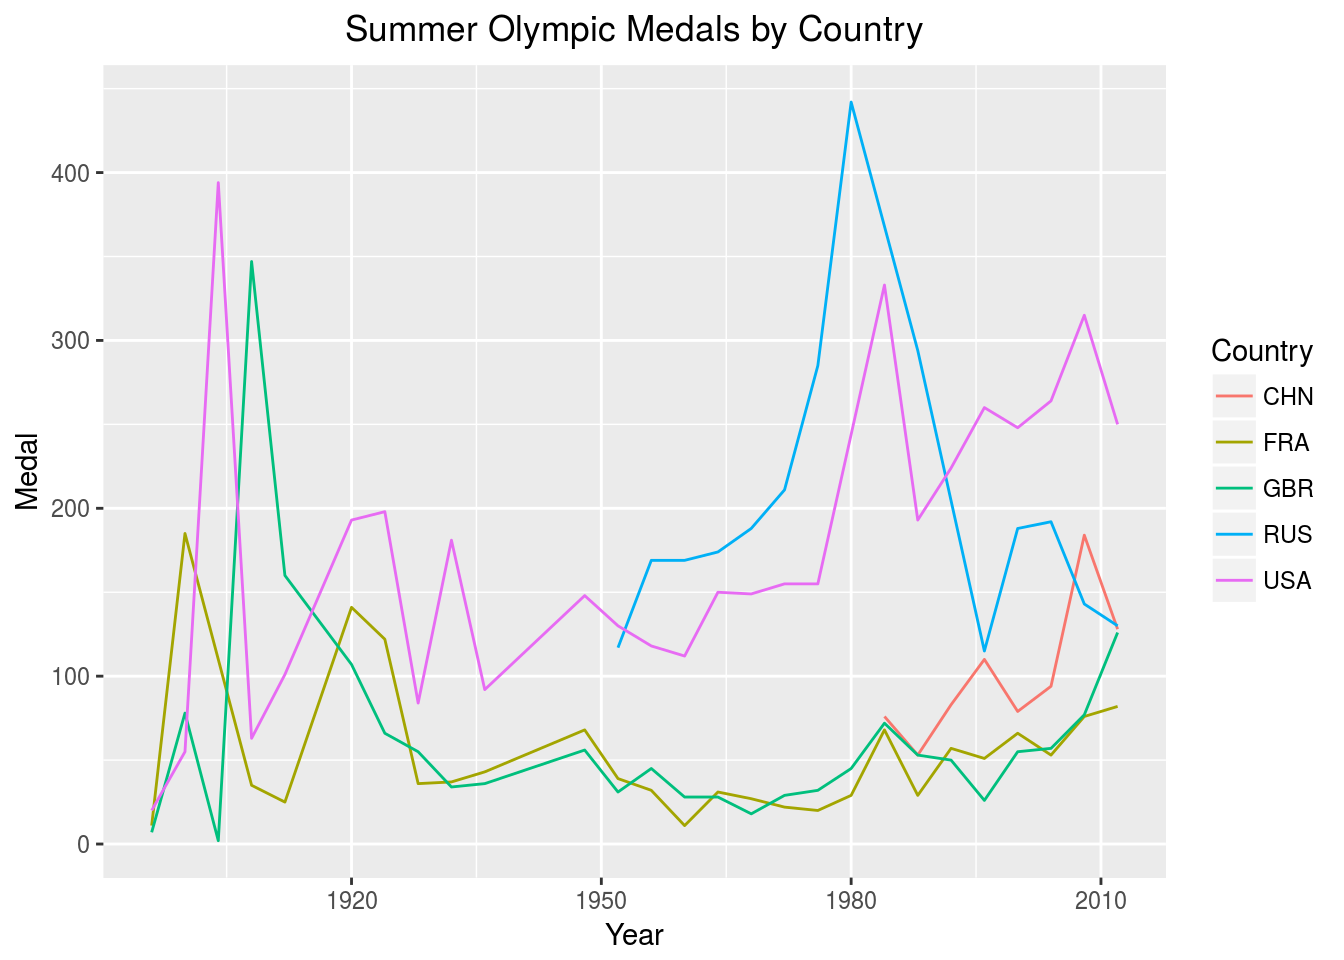
\includegraphics{bookdown-demo_files/figure-latex/unnamed-chunk-90-1.pdf}

This plot highlights a bit of the history of the summer Olympics. Note
that Russia began competing in the 1950s, and China didn't begin
competing until the mid-1980s. While the US has the longest sustained
volume, Russia has the highest number in a single year (1980). While
Great Britain had a surge at the turn of the century, it decreased to
\textasciitilde{}50 medals in the 1920s and stayed near this mark for
most of the century (as has France).

\section{Practice Problem}\label{practice-problem-2}

Using the Olympic Data and Google, try to recreate the plot below with a
horizontal barplot and bars ordered by volume of medals.

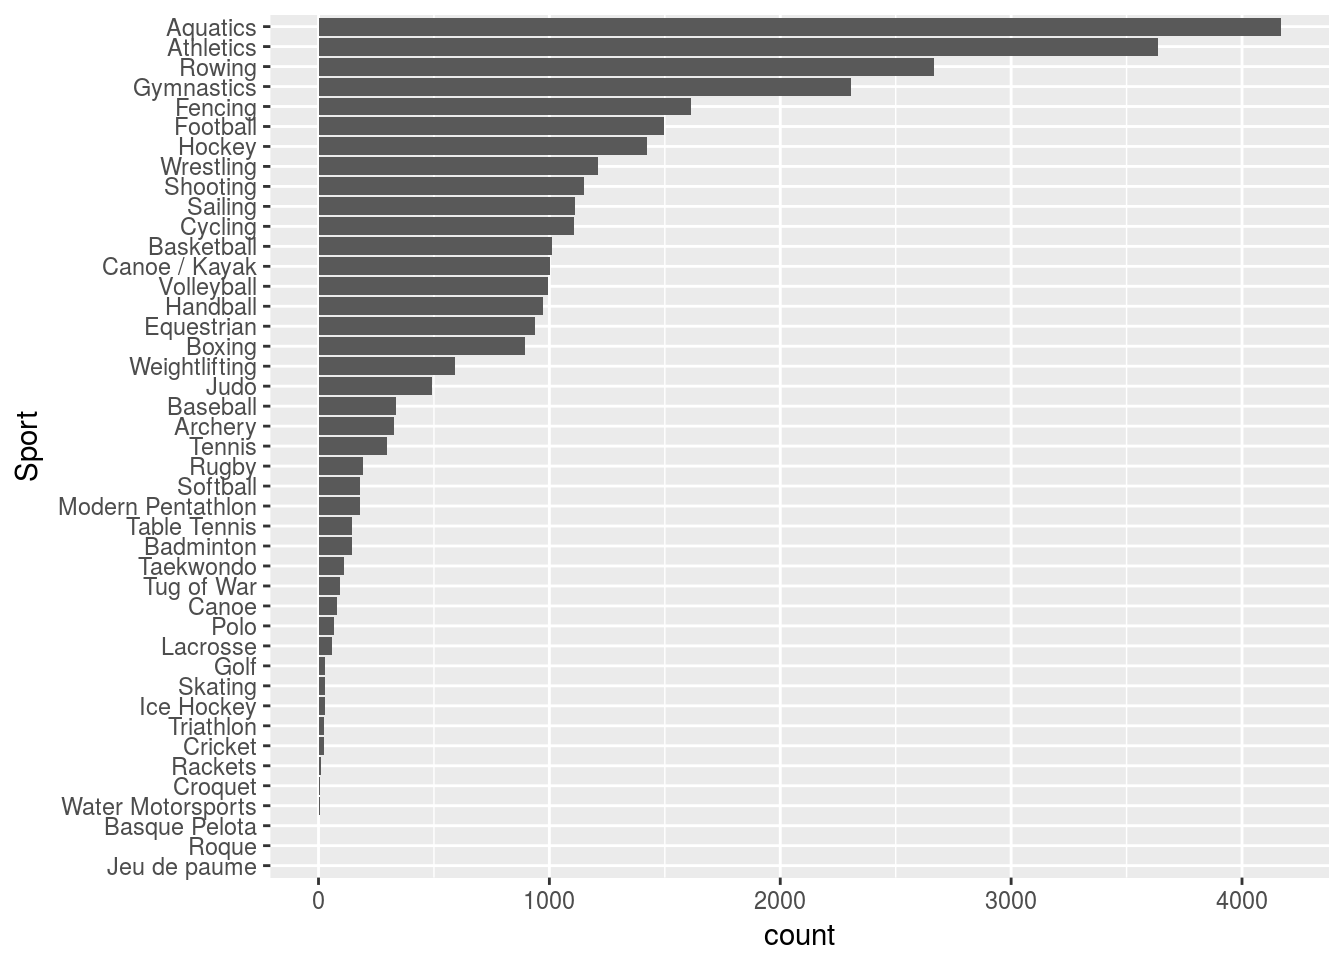
\includegraphics{bookdown-demo_files/figure-latex/unnamed-chunk-91-1.pdf}

Do your best to work this out on your own, but if you get stuck, use
these hints to help you figure out what to do next.

\begin{center}\rule{0.5\linewidth}{\linethickness}\end{center}

\subsection{Hint \#1}\label{hint-1}

\begin{enumerate}
\def\labelenumi{\arabic{enumi})}
\tightlist
\item
  The plot above indicates we will need medal counts by sport. We've
  done this before with the Korean Conflict data. Let's adapt that code
  for our new purpose.
\end{enumerate}

\begin{verbatim}
# This code produced a histogram of Korean Conflict casualties 
# grouped by branch of service.

ggplot(kor, aes(BRANCH)) + geom_bar()
\end{verbatim}

\begin{Shaded}
\begin{Highlighting}[]
\CommentTok{# Our new code should produce a histogram of Olympic medal winners }
\CommentTok{# grouped by sport.}
\KeywordTok{ggplot}\NormalTok{(oly, }\KeywordTok{aes}\NormalTok{(Sport)) +}\StringTok{ }\KeywordTok{geom_bar}\NormalTok{()}
\end{Highlighting}
\end{Shaded}

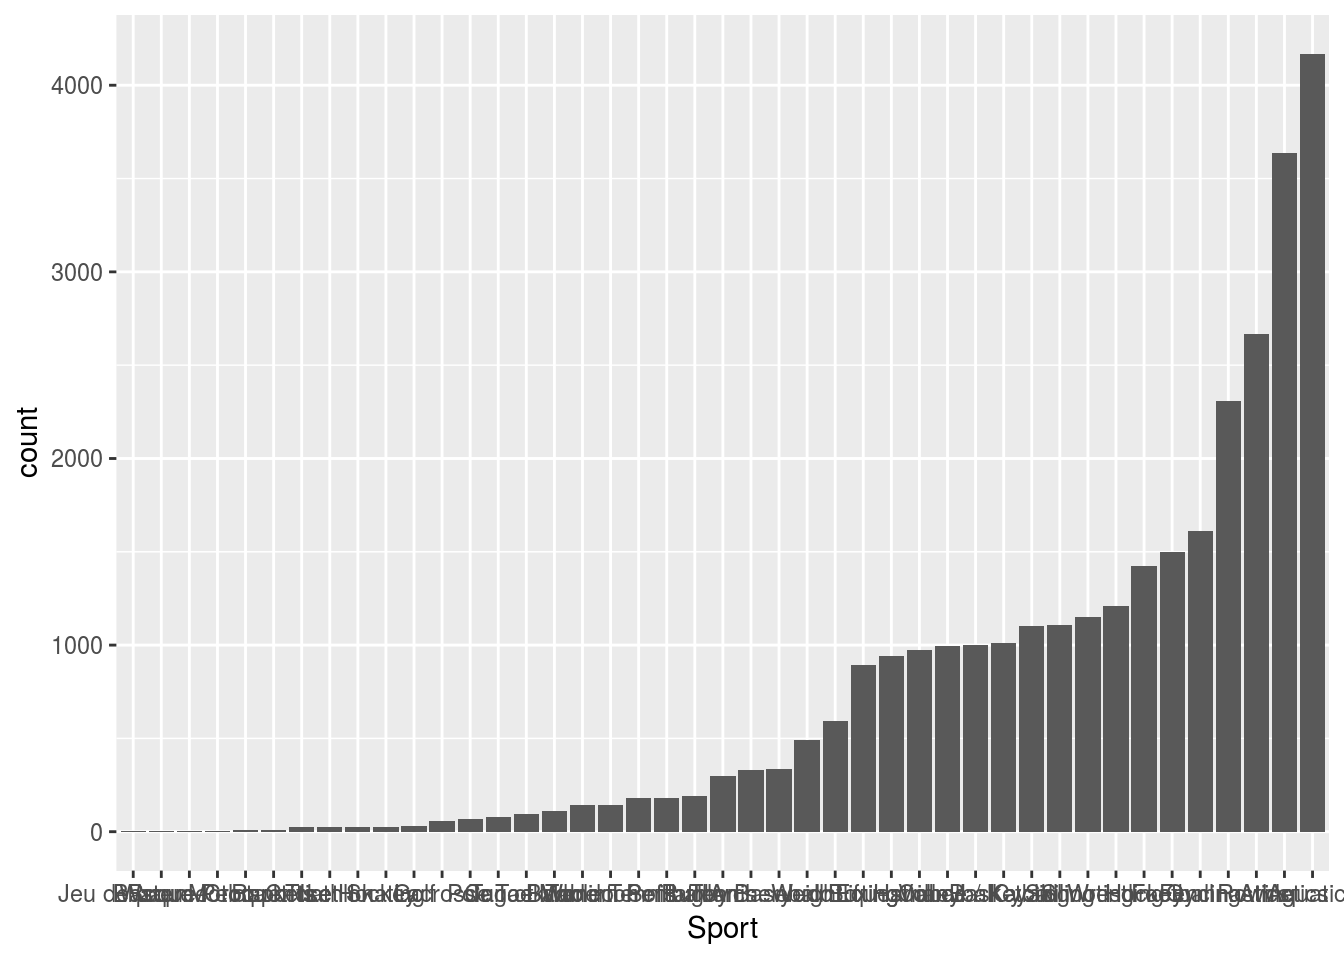
\includegraphics{bookdown-demo_files/figure-latex/unnamed-chunk-92-1.pdf}

We're not there yet, but we're on the right track!

\begin{center}\rule{0.5\linewidth}{\linethickness}\end{center}

\subsection{Hint \#2}\label{hint-2}

\begin{enumerate}
\def\labelenumi{\arabic{enumi})}
\setcounter{enumi}{1}
\tightlist
\item
  Let's figure out the horizontal requirement for this histogram. This
  is a good time to point out some RStudio cheatsheets that are
  accessible from your RStudio interface. Go to the \texttt{Help} menu
  in RStudio, click \texttt{Cheatsheets}, and select the
  \texttt{Data\ Visualization\ with\ ggplot2} link. If you explore this
  sheet and/or do some quick Googling (``horizontal barplot in
  ggplot2''), you'll find the command \texttt{coord\_flip()}.
\end{enumerate}

\begin{Shaded}
\begin{Highlighting}[]
\KeywordTok{ggplot}\NormalTok{(oly, }\KeywordTok{aes}\NormalTok{(Sport)) +}\StringTok{ }\KeywordTok{geom_bar}\NormalTok{() +}\StringTok{ }\KeywordTok{coord_flip}\NormalTok{()}
\end{Highlighting}
\end{Shaded}

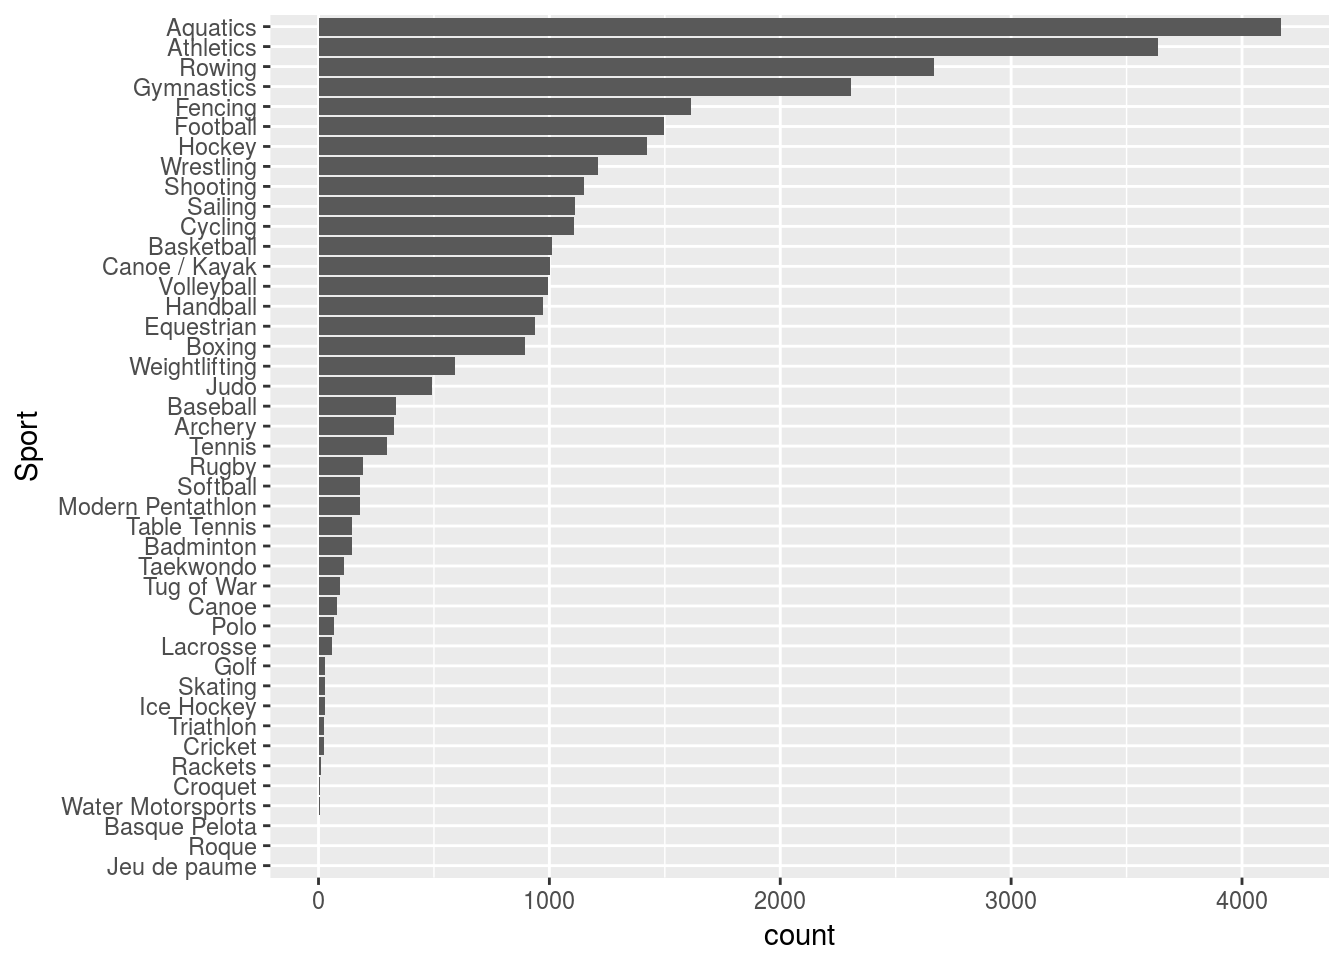
\includegraphics{bookdown-demo_files/figure-latex/unnamed-chunk-93-1.pdf}

\begin{center}\rule{0.5\linewidth}{\linethickness}\end{center}

\subsection{Hint \#3}\label{hint-3}

\begin{enumerate}
\def\labelenumi{\arabic{enumi})}
\setcounter{enumi}{2}
\tightlist
\item
  The example plot has blue bars. Let's change that in our plot. Our
  cheatsheet says the \texttt{geom\_bar()} command has \texttt{color}
  and \texttt{fill} options we could explore. It looks like
  \texttt{color} is the color of the rectangle edges, and \texttt{fill}
  is the color inside the rectangles. Let's use a white border and a
  gray fill.
\end{enumerate}

\begin{Shaded}
\begin{Highlighting}[]
\KeywordTok{ggplot}\NormalTok{(oly, }\KeywordTok{aes}\NormalTok{(Sport)) +}\StringTok{ }\KeywordTok{geom_bar}\NormalTok{(}\DataTypeTok{color=}\StringTok{"white"}\NormalTok{, }\DataTypeTok{fill=}\StringTok{"blue"}\NormalTok{) +}\StringTok{ }\KeywordTok{coord_flip}\NormalTok{()}
\end{Highlighting}
\end{Shaded}

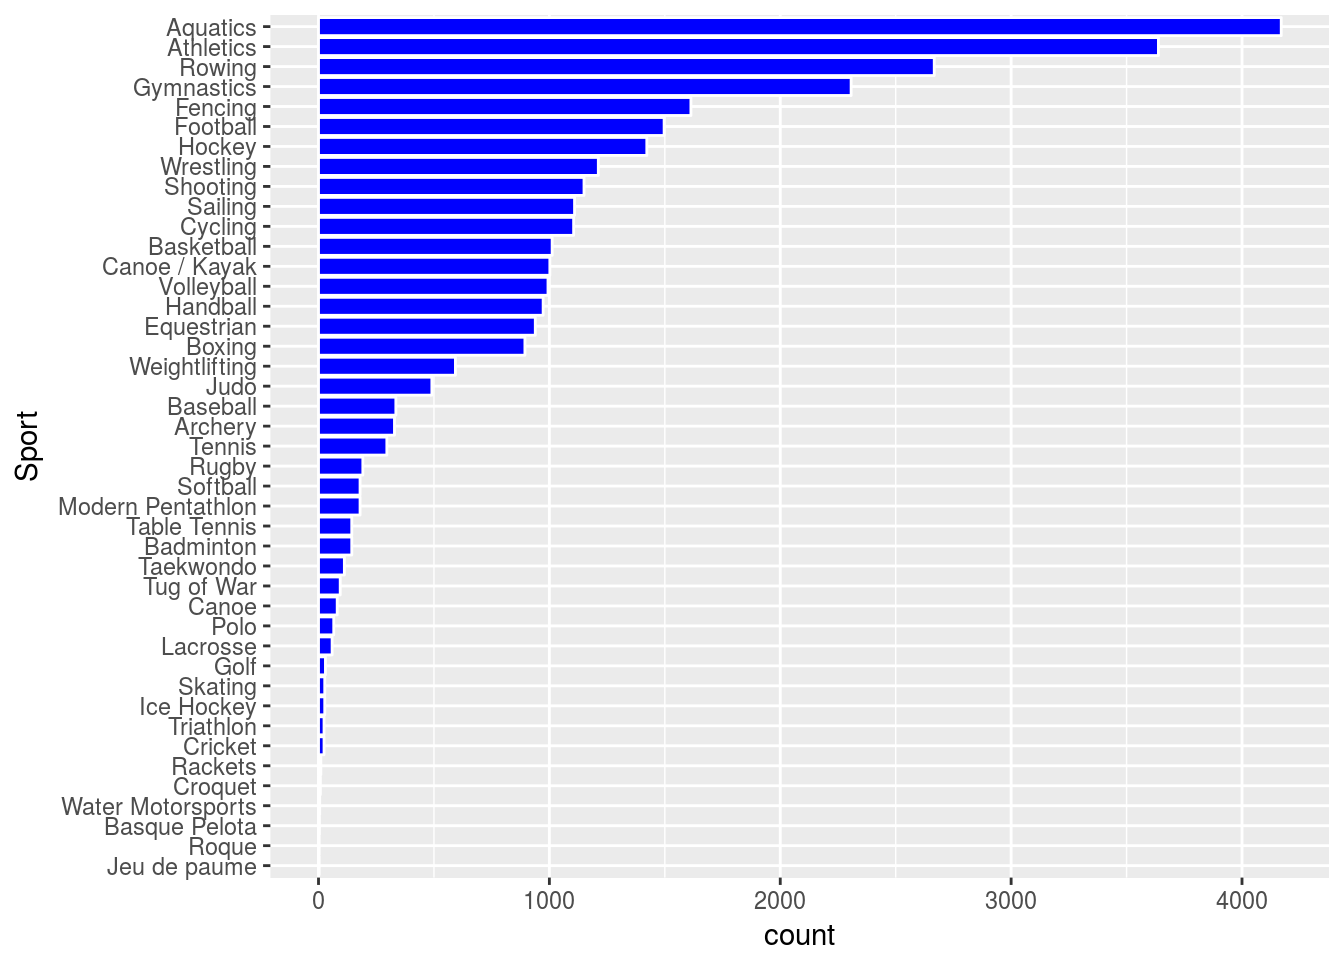
\includegraphics{bookdown-demo_files/figure-latex/unnamed-chunk-94-1.pdf}

It starting to look pretty good now. Let's polish this plot with a title
and better axes labels.

\begin{center}\rule{0.5\linewidth}{\linethickness}\end{center}

\subsection{Hint \#4}\label{hint-4}

\begin{enumerate}
\def\labelenumi{\arabic{enumi})}
\setcounter{enumi}{3}
\tightlist
\item
  We have plenty of previous examples to copy some good title and axis
  label code. We can make our new plot look even better than the one
  we're trying to replicate.
\end{enumerate}

\begin{Shaded}
\begin{Highlighting}[]
\CommentTok{# Note: the Medal Count is shown as the "ylab" instead }
\CommentTok{# of "xlab" because we used coord_flip()}
\KeywordTok{ggplot}\NormalTok{(oly, }\KeywordTok{aes}\NormalTok{(Sport)) +}\StringTok{ }\KeywordTok{geom_bar}\NormalTok{(}\DataTypeTok{color=}\StringTok{"white"}\NormalTok{, }\DataTypeTok{fill=}\StringTok{"blue"}\NormalTok{) +}\StringTok{ }\KeywordTok{coord_flip}\NormalTok{() +}
\StringTok{  }\KeywordTok{ggtitle}\NormalTok{(}\StringTok{'Summer Olympic Medals by Sport'}\NormalTok{) +}\StringTok{ }
\StringTok{  }\KeywordTok{theme}\NormalTok{(}\DataTypeTok{plot.title =} \KeywordTok{element_text}\NormalTok{(}\DataTypeTok{hjust =} \FloatTok{0.5}\NormalTok{)) +}\StringTok{ }
\StringTok{  }\KeywordTok{ylab}\NormalTok{(}\StringTok{"Medal Count"}\NormalTok{)}
\end{Highlighting}
\end{Shaded}

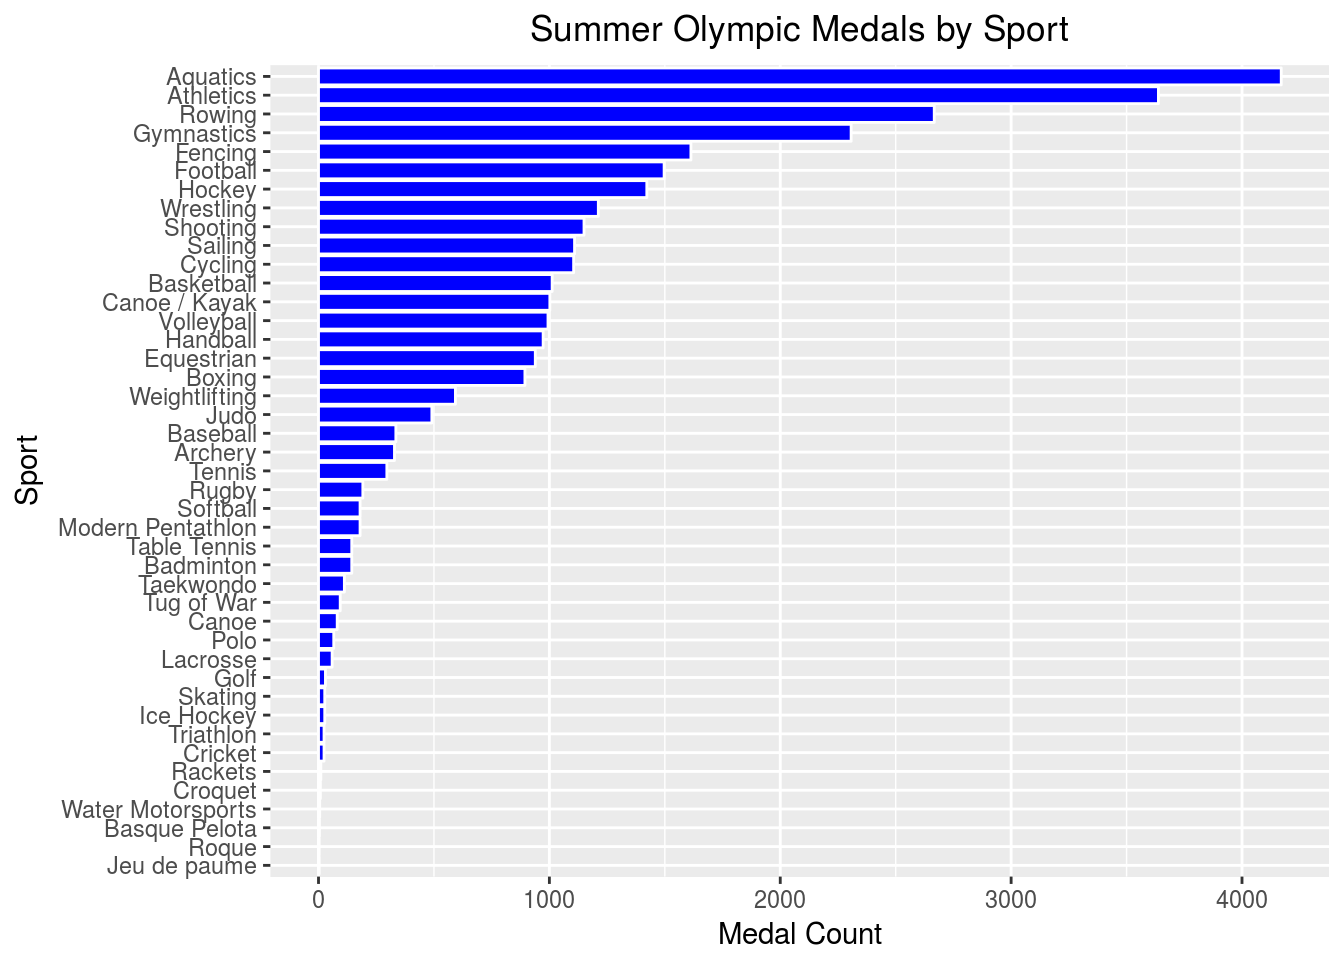
\includegraphics{bookdown-demo_files/figure-latex/unnamed-chunk-95-1.pdf}

Mission accomplished!

\chapter{Introduction to Control
Structures}\label{introduction-to-control-structures}

This lesson will cover the \texttt{if()} statement as well as the
\texttt{for()} loop and \texttt{while()} loop. These are three very
common control structures for all computer programming languages and are
used extensively in the R programming language.

\section{if() Statements}\label{if-statements}

The \texttt{if()} statement allows us to automate decision points and
guide the computer through a data flow diagram. The basic syntax is
given below:

\begin{Shaded}
\begin{Highlighting}[]
\NormalTok{if(<condition>) \{}
  \CommentTok{# do something}
\NormalTok{\} else if(<another condition>)\{}
  \CommentTok{# do something else}
\NormalTok{\} else \{}
  \CommentTok{# do something completely different}
\NormalTok{\}}
\end{Highlighting}
\end{Shaded}

Let's see this in practice:

\begin{itemize}
\tightlist
\item
  Case 1
\end{itemize}

\begin{Shaded}
\begin{Highlighting}[]
\NormalTok{my.number =}\StringTok{ }\DecValTok{1}
\NormalTok{if(!}\KeywordTok{is.numeric}\NormalTok{(my.number)) \{}
  \KeywordTok{print}\NormalTok{(}\StringTok{"You were supposed to store a number in 'my.number'."}\NormalTok{)}
\NormalTok{\} else if(my.number >=}\StringTok{ }\DecValTok{10}\NormalTok{)\{}
  \KeywordTok{print}\NormalTok{(}\StringTok{"My number is greater than or equal to 10."}\NormalTok{)}
\NormalTok{\} else \{}
  \KeywordTok{print}\NormalTok{(}\StringTok{"My number is less than 10."}\NormalTok{)}
\NormalTok{\}}
\end{Highlighting}
\end{Shaded}

\begin{verbatim}
## [1] "My number is less than 10."
\end{verbatim}

\begin{itemize}
\tightlist
\item
  Case 2
\end{itemize}

\begin{Shaded}
\begin{Highlighting}[]
\NormalTok{my.number =}\StringTok{ }\DecValTok{100}
\NormalTok{if(!}\KeywordTok{is.numeric}\NormalTok{(my.number)) \{}
  \KeywordTok{print}\NormalTok{(}\StringTok{"You were supposed to store a number in 'my.number'."}\NormalTok{)}
\NormalTok{\} else if(my.number >=}\StringTok{ }\DecValTok{10}\NormalTok{)\{}
  \KeywordTok{print}\NormalTok{(}\StringTok{"My number is greater than or equal to 10."}\NormalTok{)}
\NormalTok{\} else \{}
  \KeywordTok{print}\NormalTok{(}\StringTok{"My number is less than 10."}\NormalTok{)}
\NormalTok{\}}
\end{Highlighting}
\end{Shaded}

\begin{verbatim}
## [1] "My number is greater than or equal to 10."
\end{verbatim}

\begin{itemize}
\tightlist
\item
  Case 3
\end{itemize}

\begin{Shaded}
\begin{Highlighting}[]
\NormalTok{my.number =}\StringTok{ "huge"}
\NormalTok{if(!}\KeywordTok{is.numeric}\NormalTok{(my.number)) \{}
  \KeywordTok{print}\NormalTok{(}\StringTok{"You were supposed to store a number in 'my.number'."}\NormalTok{)}
\NormalTok{\} else if(my.number >=}\StringTok{ }\DecValTok{10}\NormalTok{)\{}
  \KeywordTok{print}\NormalTok{(}\StringTok{"My number is greater than or equal to 10."}\NormalTok{)}
\NormalTok{\} else \{}
  \KeywordTok{print}\NormalTok{(}\StringTok{"My number is less than 10."}\NormalTok{)}
\NormalTok{\}}
\end{Highlighting}
\end{Shaded}

\begin{verbatim}
## [1] "You were supposed to store a number in 'my.number'."
\end{verbatim}

The \texttt{else} clause(s) can grow rather lengthy if many special
cases must be handled uniquely, but it is quite often the case that we
just need an \texttt{if()} statement. Think of this statement as a gate
you must pass in order to run a chunk of code.

\begin{Shaded}
\begin{Highlighting}[]
\NormalTok{if(<condition>) \{}
  \NormalTok{## do something}
\NormalTok{\}}
\end{Highlighting}
\end{Shaded}

An example you might use in practice is boundary checking. Suppose you
have age data, and you want to be notified if there is a negative age
recorded.

\begin{Shaded}
\begin{Highlighting}[]
\NormalTok{my.age <-}\StringTok{ }\DecValTok{1}
\NormalTok{if(my.age <}\StringTok{ }\DecValTok{0}\NormalTok{) \{}
  \KeywordTok{print}\NormalTok{(}\StringTok{"Negative age detected.  Check for data entry error."}\NormalTok{)}
\NormalTok{\}}
\end{Highlighting}
\end{Shaded}

We didn't see our notification because we didn't pass the \texttt{if()}
gate that reaches the \texttt{print()} command. We skipped right over
it.

\begin{Shaded}
\begin{Highlighting}[]
\NormalTok{my.age <-}\StringTok{ }\NormalTok{-}\DecValTok{1}
\NormalTok{if(my.age <}\StringTok{ }\DecValTok{0}\NormalTok{) \{}
  \KeywordTok{print}\NormalTok{(}\StringTok{"Negative age detected.  Check for data entry error."}\NormalTok{)}
\NormalTok{\}}
\end{Highlighting}
\end{Shaded}

\begin{verbatim}
## [1] "Negative age detected.  Check for data entry error."
\end{verbatim}

Now we get the message because we passed the \texttt{if()} condition.

The \texttt{if()} statement is most often used in \emph{loops} and
\emph{functions}. We'll illustrate the use of the \texttt{if()}
statement in \emph{loops} below.

\section{Loops}\label{loops}

Loops provide a way to systematically walk down a data structure
(usually a vector, data frame, or list) and potentially accomplish a
task many times along the way. The \texttt{for()} loop and the
\texttt{while()} loop will be the primary loops used in this class. The
\texttt{for()} loop is used when we know ahead of time a finite number
of iterations that we need to execute. For example, we might execute a
task for every object in a vector/list or every row in a data frame.

The \texttt{for()} loop below iterates over the values 1, 2, 3, 4, and 5
and prints each of the values.

\begin{Shaded}
\begin{Highlighting}[]
\NormalTok{for(i in }\DecValTok{1}\NormalTok{:}\DecValTok{5}\NormalTok{)\{}
  \KeywordTok{print}\NormalTok{(i)}
\NormalTok{\}}
\end{Highlighting}
\end{Shaded}

\begin{verbatim}
## [1] 1
## [1] 2
## [1] 3
## [1] 4
## [1] 5
\end{verbatim}

Notice that we can also use \texttt{i} to access a value in a vector, a
row in a data frame, or an object in a list.

\begin{Shaded}
\begin{Highlighting}[]
\NormalTok{letters <-}\StringTok{ }\KeywordTok{c}\NormalTok{(}\StringTok{"a"}\NormalTok{, }\StringTok{"b"}\NormalTok{, }\StringTok{"c"}\NormalTok{, }\StringTok{"d"}\NormalTok{, }\StringTok{"e"}\NormalTok{)}
\NormalTok{for(i in }\DecValTok{1}\NormalTok{:}\DecValTok{5}\NormalTok{)\{}
  \KeywordTok{print}\NormalTok{(letters[i])}
\NormalTok{\}}
\end{Highlighting}
\end{Shaded}

\begin{verbatim}
## [1] "a"
## [1] "b"
## [1] "c"
## [1] "d"
## [1] "e"
\end{verbatim}

You also don't have to start with 1 or use the letter \emph{i}:

\begin{Shaded}
\begin{Highlighting}[]
\NormalTok{for (year in }\DecValTok{2010}\NormalTok{:}\DecValTok{2015}\NormalTok{)\{}
  \KeywordTok{print}\NormalTok{(}\KeywordTok{paste}\NormalTok{(}\StringTok{"The year is"}\NormalTok{, year))}
\NormalTok{\}}
\end{Highlighting}
\end{Shaded}

\begin{verbatim}
## [1] "The year is 2010"
## [1] "The year is 2011"
## [1] "The year is 2012"
## [1] "The year is 2013"
## [1] "The year is 2014"
## [1] "The year is 2015"
\end{verbatim}

The \texttt{next} command is often used to skip an iteration if a
certain condition is met. The code below illustrates how to use
\texttt{next}:

\begin{Shaded}
\begin{Highlighting}[]
\NormalTok{for(i in }\DecValTok{1}\NormalTok{:}\DecValTok{5}\NormalTok{)\{}
  \NormalTok{if(letters[i]==}\StringTok{"c"}\NormalTok{)\{}
    \NormalTok{next}
  \NormalTok{\}}
  \KeywordTok{print}\NormalTok{(letters[i])}
\NormalTok{\}}
\end{Highlighting}
\end{Shaded}

\begin{verbatim}
## [1] "a"
## [1] "b"
## [1] "d"
## [1] "e"
\end{verbatim}

Loops can also be nested inside of each other. This is useful when
working with multiple dimensions (like matrices) or lists of lists. For
example, the outer \texttt{for()} loop iterates over countries, and the
inner \texttt{for()} loop iterates over each city in a given country. An
example of a nested \texttt{for()} loop is given below, creating a
multiplication table:

\begin{Shaded}
\begin{Highlighting}[]
\CommentTok{# nested for: multiplication table}
\CommentTok{# create a 10 x 10 matrix (10 rows and 10 columns)}
\NormalTok{mymat =}\StringTok{ }\KeywordTok{matrix}\NormalTok{(}\DataTypeTok{nrow=}\DecValTok{10}\NormalTok{, }\DataTypeTok{ncol=}\DecValTok{10}\NormalTok{) }

\NormalTok{for(i in }\DecValTok{1}\NormalTok{:}\KeywordTok{nrow}\NormalTok{(mymat)) \{  }\CommentTok{# for each row}
  \NormalTok{for(j in }\DecValTok{1}\NormalTok{:}\KeywordTok{ncol}\NormalTok{(mymat))\{ }\CommentTok{# for each column}
    \CommentTok{# assign values based on position: product of two indices}
    \NormalTok{mymat[i,j] =}\StringTok{ }\NormalTok{i*j     }
  \NormalTok{\}}
\NormalTok{\}}

\NormalTok{mymat}
\end{Highlighting}
\end{Shaded}

\begin{verbatim}
##       [,1] [,2] [,3] [,4] [,5] [,6] [,7] [,8] [,9] [,10]
##  [1,]    1    2    3    4    5    6    7    8    9    10
##  [2,]    2    4    6    8   10   12   14   16   18    20
##  [3,]    3    6    9   12   15   18   21   24   27    30
##  [4,]    4    8   12   16   20   24   28   32   36    40
##  [5,]    5   10   15   20   25   30   35   40   45    50
##  [6,]    6   12   18   24   30   36   42   48   54    60
##  [7,]    7   14   21   28   35   42   49   56   63    70
##  [8,]    8   16   24   32   40   48   56   64   72    80
##  [9,]    9   18   27   36   45   54   63   72   81    90
## [10,]   10   20   30   40   50   60   70   80   90   100
\end{verbatim}

The \texttt{while()} loop is used when we don't know how many iterations
we need to go through, but we know the condition that needs to be met
before we are done.

\begin{Shaded}
\begin{Highlighting}[]
\NormalTok{i <-}\StringTok{ }\DecValTok{5}
\NormalTok{while(i <=}\StringTok{ }\DecValTok{25}\NormalTok{) \{}
  \KeywordTok{print}\NormalTok{(i)}
  \CommentTok{# Here we set a new value of i.}
  \NormalTok{i <-}\StringTok{ }\NormalTok{i +}\StringTok{ }\DecValTok{5}
  \CommentTok{# Now we go back and check the while() condition.}
\NormalTok{\}}
\end{Highlighting}
\end{Shaded}

\begin{verbatim}
## [1] 5
## [1] 10
## [1] 15
## [1] 20
## [1] 25
\end{verbatim}

To finish out this lesson, we'll provide an example of some more
sophisticated code. This function simulates a round of play in the board
game \emph{RISK}. In the board game \emph{RISK}, an attacker begins an
assault against a defender, and the win/loss is adjudicated as both
players begin rolling dice and comparing values. The simulation below
plays through this entire series, declares whether the attacker or the
defender won, and declares the number of armies left on the board for
each player. Instead of doing this once, this code plays through this
10,000 times, and in the process calculates the probability of the
\emph{attacker} winning. This type of process is known as Monte Carlo
Simulation. While you may not fully understand all aspects of this code,
note throughout this function how important \emph{loops} and
\texttt{if()} statements are:

\begin{Shaded}
\begin{Highlighting}[]
\CommentTok{# Our function will take as inputs the number of armies the }
\CommentTok{# attacker has, the number of armies the defender has, and }
\CommentTok{# the desired number of simulated trials the user wants.}
\NormalTok{risk <-}\StringTok{ }\NormalTok{function(attacker, defender, n) \{}
  \CommentTok{# Create an empty vector to hold the simulated win/loss outcomes.}
  \NormalTok{results <-}\StringTok{ }\KeywordTok{rep}\NormalTok{(}\OtherTok{NA}\NormalTok{, n)}
  \CommentTok{# Create restoration values to reset the armies after each trial.}
  \NormalTok{attacker.reset <-}\StringTok{ }\NormalTok{attacker}
  \NormalTok{defender.reset <-}\StringTok{ }\NormalTok{defender}
  \CommentTok{# For n total trials... }
  \NormalTok{for(j in }\DecValTok{1}\NormalTok{:n)\{}
    \CommentTok{# Reset the attacker and defender for a new trial.}
    \NormalTok{attacker <-}\StringTok{ }\NormalTok{attacker.reset}
    \NormalTok{defender <-}\StringTok{ }\NormalTok{defender.reset}
    \CommentTok{# ...as long as the attacker has more than one army}
    \CommentTok{# and the defender has an army...}
    \NormalTok{while(attacker >}\StringTok{ }\DecValTok{1} \NormalTok{&}\StringTok{ }\NormalTok{defender >}\StringTok{ }\DecValTok{0}\NormalTok{) \{}
      \CommentTok{# Both players pick up the right number of dice...}
      \NormalTok{atk.dice <-}\StringTok{ }\KeywordTok{min}\NormalTok{(attacker}\DecValTok{-1}\NormalTok{, }\DecValTok{3}\NormalTok{)}
      \NormalTok{def.dice <-}\StringTok{ }\KeywordTok{min}\NormalTok{(defender, }\DecValTok{2}\NormalTok{)}
      \CommentTok{# Both players roll the right number of dice...}
      \NormalTok{atk.roll <-}\StringTok{ }\KeywordTok{ceiling}\NormalTok{(}\KeywordTok{runif}\NormalTok{(atk.dice)*}\DecValTok{6}\NormalTok{)}
      \NormalTok{def.roll <-}\StringTok{ }\KeywordTok{ceiling}\NormalTok{(}\KeywordTok{runif}\NormalTok{(def.dice)*}\DecValTok{6}\NormalTok{)}
      \CommentTok{# Each player's dice are sorted from greatest to least...}
      \NormalTok{atk.roll <-}\StringTok{ }\NormalTok{atk.roll[}\KeywordTok{order}\NormalTok{(atk.roll,}\DataTypeTok{decreasing=}\NormalTok{T)]}
      \NormalTok{def.roll <-}\StringTok{ }\NormalTok{def.roll[}\KeywordTok{order}\NormalTok{(def.roll,}\DataTypeTok{decreasing=}\NormalTok{T)]}
      \CommentTok{# Compare the correct numbers of dice for each player...}
      \NormalTok{comparison <-}\StringTok{ }\KeywordTok{min}\NormalTok{(atk.dice, def.dice)}
      \NormalTok{for (i in }\DecValTok{1}\NormalTok{:comparison) \{}
        \NormalTok{if (atk.roll[i] >}\StringTok{ }\NormalTok{def.roll[i])\{}
          \CommentTok{# The attacker won, so the defender loses an army...}
          \NormalTok{defender <-}\StringTok{ }\NormalTok{defender}\DecValTok{-1}
        \NormalTok{\}}
        \NormalTok{if (atk.roll[i] <=}\StringTok{ }\NormalTok{def.roll[i])\{}
          \CommentTok{# The defender won, so the attacker loses an army...}
          \NormalTok{attacker <-}\StringTok{ }\NormalTok{attacker}\DecValTok{-1}
        \NormalTok{\}}
        \CommentTok{# Keep going up to the number of required comparisons.}
      \NormalTok{\}}
      \CommentTok{# Keep going until the attacker or defender is wiped out.}
    \NormalTok{\}}
    \CommentTok{# If the defender ran out of armies, the attacker wins.}
    \NormalTok{if (defender==}\DecValTok{0}\NormalTok{) results[j] <-}\StringTok{ "Attacker"}
    \CommentTok{# If the defender did not run out of armies, the defender wins.}
    \NormalTok{if (defender>}\DecValTok{0}\NormalTok{) results[j] <-}\StringTok{ "Defender"}
    \CommentTok{# Keep going up to the number of required trials.}
  \NormalTok{\}}
  \KeywordTok{print}\NormalTok{(}\KeywordTok{paste}\NormalTok{(}\StringTok{"The Probability of the Attacker winning is:"}\NormalTok{,}
              \KeywordTok{length}\NormalTok{(results[results==}\StringTok{"Attacker"}\NormalTok{])/n))}
\NormalTok{\}}
\end{Highlighting}
\end{Shaded}

The statement below illustrates how to use the \texttt{risk()} function:

\begin{Shaded}
\begin{Highlighting}[]
\KeywordTok{risk}\NormalTok{(}\DataTypeTok{attacker=}\DecValTok{4}\NormalTok{,}\DataTypeTok{defender=}\DecValTok{3}\NormalTok{,}\DataTypeTok{n=}\DecValTok{1000}\NormalTok{)}
\end{Highlighting}
\end{Shaded}

\begin{verbatim}
## [1] "The Probability of the Attacker winning is: 0.456"
\end{verbatim}

\section{Practice Problem}\label{practice-problem-3}

Use the instructions below to determine and visualize the average movie
rating by genre.

\begin{itemize}
\tightlist
\item
  Read the movie ratings data you downloaded in Section 1.6 into R.
\item
  Use the code below to build a vector called \texttt{genres} that
  contains all unique genre names contained in the data set.
\end{itemize}

\begin{Shaded}
\begin{Highlighting}[]
\KeywordTok{library}\NormalTok{(stringr)}
\NormalTok{rating <-}\StringTok{ }\KeywordTok{read.csv}\NormalTok{(}\StringTok{"rating2.csv"}\NormalTok{, }\DataTypeTok{as.is =} \OtherTok{TRUE}\NormalTok{)}
\NormalTok{genre.list <-}\StringTok{ }\KeywordTok{unique}\NormalTok{(}\KeywordTok{unlist}\NormalTok{(}\KeywordTok{str_split}\NormalTok{(rating$genres,}\StringTok{"}\CharTok{\textbackslash{}\textbackslash{}}\StringTok{|"}\NormalTok{)))}
\end{Highlighting}
\end{Shaded}

Try to execute the following steps before looking at the code solution
that shows just one way to accomplish this task.

\begin{itemize}
\tightlist
\item
  Create a vector object that is the same length as \texttt{genre.list}
  to contain the \texttt{mean} ratings.
\item
  Iterate over your original data set in a \texttt{for()} loop, use the
  \texttt{grep()} command to extract the subset that is related to a
  specific genre, and calculate the mean rating for that genre.
\item
  Create a barplot visualization of average ratings by genre.
\end{itemize}

\begin{center}\rule{0.5\linewidth}{\linethickness}\end{center}

\subsection{Hint \#1}\label{hint-1-1}

\begin{itemize}
\tightlist
\item
  Create a vector object that is the same length as \texttt{genre.list}
  to contain the \texttt{mean} ratings.
\end{itemize}

The \texttt{rep()} command replicates a value or set of values a
specified number of times. The \texttt{length()} command returns the
number of elements in a vector or list object. We can use these two
functions to create a vector of the correct length.

\begin{Shaded}
\begin{Highlighting}[]
\CommentTok{# We'll replicate NA as our placeholder to be replaced by actual numbers.}
\NormalTok{mean.ratings <-}\StringTok{ }\KeywordTok{rep}\NormalTok{(}\OtherTok{NA}\NormalTok{,}\KeywordTok{length}\NormalTok{(genre.list))}
\end{Highlighting}
\end{Shaded}

\begin{center}\rule{0.5\linewidth}{\linethickness}\end{center}

\subsection{Hint \#2}\label{hint-2-1}

\begin{itemize}
\tightlist
\item
  Iterate over your original data set in a \texttt{for()} loop, use the
  \texttt{grep()} command to extract the subset that is related to a
  specific genre, and calculate the mean rating for that genre. Note
  that many movies are classified as belonging to multiple genres, and
  we will allow each movie's rating to contribute to the calculation of
  the mean rating for any genre to which it belongs.
\end{itemize}

\begin{Shaded}
\begin{Highlighting}[]
\CommentTok{# It appears most movies are associated with multiple genres.}
\KeywordTok{head}\NormalTok{(rating$genres)}
\end{Highlighting}
\end{Shaded}

\begin{verbatim}
## [1] "Adventure|Animation|Children|Comedy|Fantasy"    
## [2] "Action|Drama|War"                               
## [3] "Action|Adventure|Sci-Fi"                        
## [4] "Adventure|Animation|Children|Drama|Musical|IMAX"
## [5] "Drama|War"                                      
## [6] "Adventure|Animation|Children|Comedy|Musical"
\end{verbatim}

We might be tempted to set up our \texttt{for()} loop from
\texttt{1:length(rating)}, but that would only loop over the 7 objects
inside our \texttt{rating} data frame. We might also be tempted to loop
over the 283,886 movies, which we can do by looping over any column of
\texttt{rating} (e.g, \texttt{1:length(rating\$title)}. What we really
want to do is loop over our vector of genres (i.e.,
\texttt{1:length(genre.list)}). This approach will let us complete an
assessment of each genre all at once instead of moving through our list
movie by movie.

\begin{Shaded}
\begin{Highlighting}[]
\CommentTok{# We'll iterate over our vector of genres.}
\NormalTok{for(i in }\DecValTok{1}\NormalTok{:}\KeywordTok{length}\NormalTok{(genre.list))\{}
  \CommentTok{# Let's filter out any movies that don't belong to the genre of interest.}
  \CommentTok{# First identify which movie indices correspond to the genre of interest.}
  \NormalTok{this.genre.indices <-}\StringTok{ }\KeywordTok{grep}\NormalTok{(genre.list[i],rating$genres)}
  \CommentTok{# Now let's compute and store the mean rating of this genre.}
  \CommentTok{# We'll compute the mean of "rating" column in the rows we just identifed.}
  \NormalTok{mean.ratings[i] <-}\StringTok{ }\KeywordTok{mean}\NormalTok{(rating[this.genre.indices,}\StringTok{"rating"}\NormalTok{])}
\NormalTok{\}}
\end{Highlighting}
\end{Shaded}

Now we have a vector of mean ratings, which we can combine with the
genre list into a data frame and display as text here.

\begin{Shaded}
\begin{Highlighting}[]
\NormalTok{df.rating <-}\StringTok{ }\KeywordTok{data.frame}\NormalTok{(genre.list,mean.ratings)}
\NormalTok{df.rating}
\end{Highlighting}
\end{Shaded}

\begin{verbatim}
##            genre.list mean.ratings
## 1           Adventure     3.481759
## 2           Animation     3.579487
## 3            Children     3.420384
## 4              Comedy     3.358041
## 5             Fantasy     3.464419
## 6              Action     3.452660
## 7               Drama     3.641138
## 8                 War     3.690831
## 9              Sci-Fi     3.499506
## 10            Musical     3.521342
## 11               IMAX     3.524784
## 12            Romance     3.457683
## 13             Horror     3.261698
## 14           Thriller     3.502560
## 15              Crime     3.654538
## 16            Western     3.601346
## 17            Mystery     3.639658
## 18        Documentary     3.552925
## 19          Film-Noir     3.780648
## 20 (no genres listed)     2.929924
\end{verbatim}

\begin{center}\rule{0.5\linewidth}{\linethickness}\end{center}

\subsection{Hint \#3}\label{hint-3-1}

\begin{itemize}
\tightlist
\item
  Create a barplot visualization of average ratings by genre.
\end{itemize}

We already wrote some code to do exactly this with our Olympic medal
data. Let's repurpose our old code and adjust it as necessary. Don't
reinvent the wheel!

Note: You'll see the argument \texttt{stat="identity"} in the
\texttt{geom\_bar()} command. You have the option to let R compute
means, counts, etc., from our chosen y-data. In our case, we already did
that. The \texttt{"identity"} option means we just want the values to be
presented exactly as we've provided them.

\begin{Shaded}
\begin{Highlighting}[]
\KeywordTok{library}\NormalTok{(ggplot2)}
\KeywordTok{ggplot}\NormalTok{(df.rating, }\KeywordTok{aes}\NormalTok{(}\DataTypeTok{x=}\NormalTok{genre.list,}\DataTypeTok{y=}\NormalTok{mean.ratings)) +}
\StringTok{  }\KeywordTok{geom_bar}\NormalTok{(}\DataTypeTok{stat=}\StringTok{"identity"}\NormalTok{, }\DataTypeTok{color=}\StringTok{"white"}\NormalTok{, }\DataTypeTok{fill=}\StringTok{"blue"}\NormalTok{) +}
\StringTok{  }\KeywordTok{ggtitle}\NormalTok{(}\StringTok{'Mean Movie Rating by Genre'}\NormalTok{) +}\StringTok{ }
\StringTok{  }\KeywordTok{theme}\NormalTok{(}\DataTypeTok{plot.title =} \KeywordTok{element_text}\NormalTok{(}\DataTypeTok{hjust =} \FloatTok{0.5}\NormalTok{)) +}\StringTok{ }
\StringTok{  }\KeywordTok{ylab}\NormalTok{(}\StringTok{"Mean Rating"}\NormalTok{) +}\StringTok{ }
\StringTok{  }\KeywordTok{xlab}\NormalTok{(}\StringTok{"Movie Genres"}\NormalTok{) +}\StringTok{ }
\StringTok{  }\KeywordTok{theme}\NormalTok{(}\DataTypeTok{axis.text.x =} \KeywordTok{element_text}\NormalTok{(}\DataTypeTok{angle =} \DecValTok{90}\NormalTok{, }\DataTypeTok{hjust =} \DecValTok{1}\NormalTok{))}
\end{Highlighting}
\end{Shaded}

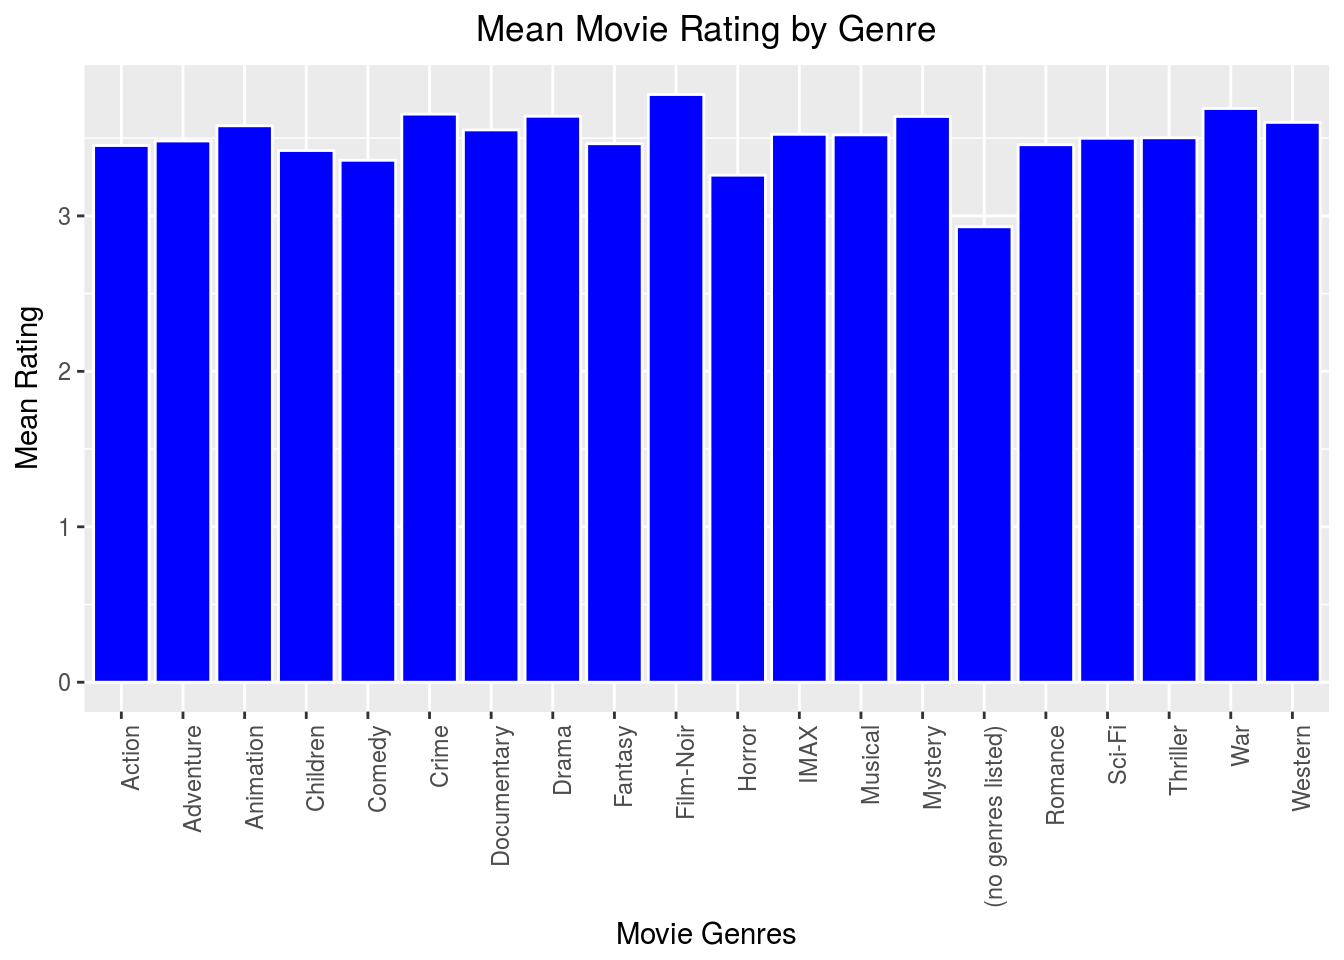
\includegraphics{bookdown-demo_files/figure-latex/unnamed-chunk-116-1.pdf}

\chapter{Introduction to Dates in R}\label{introduction-to-dates-in-r}

We often see dates and times in data. Often each record (or row) of data
is connected to at least one date or time. Similar to Microsoft Excel, R
has a special class or format that it uses to work with dates.

\section{Dates with Base R}\label{dates-with-base-r}

We will start by showing a few of the date commands that are built into
the Base R package. Later on we will take a look at the \emph{lubridate}
package \citep{R-lubridate}, which has some really handy, user-friendly
functions.

First we will demonstrate a couple commands that will generate the
current date for your system (either your physical computer or your
cloud computer). Below is the system date:

\begin{Shaded}
\begin{Highlighting}[]
\KeywordTok{Sys.Date}\NormalTok{()}
\end{Highlighting}
\end{Shaded}

\begin{verbatim}
## [1] "2017-09-14"
\end{verbatim}

Next we will show the system time down to hours, minutes, and seconds
with a Time Zone specification:

\begin{Shaded}
\begin{Highlighting}[]
\KeywordTok{Sys.time}\NormalTok{()}
\end{Highlighting}
\end{Shaded}

\begin{verbatim}
## [1] "2017-09-14 13:11:49 UTC"
\end{verbatim}

Note that these are not character objects:

\begin{Shaded}
\begin{Highlighting}[]
\KeywordTok{class}\NormalTok{(}\KeywordTok{Sys.Date}\NormalTok{())}
\end{Highlighting}
\end{Shaded}

\begin{verbatim}
## [1] "Date"
\end{verbatim}

This is a special class called the \emph{Date} class. When you read data
into R, any fields that have dates are normally converted to the
\emph{character} class, not the \emph{Date} class. In order to convert
from a \emph{character} class to the \emph{Date} class in Base R, use
the \texttt{as.Date()} command as seen below:

\begin{Shaded}
\begin{Highlighting}[]
\CommentTok{# Create a character vector of random dates}
\NormalTok{myDates <-}\StringTok{ }\KeywordTok{c}\NormalTok{(}\StringTok{"2016-02-07"}\NormalTok{, }\StringTok{"2016-04-02"}\NormalTok{,}\StringTok{"2016-06-28"}\NormalTok{)}
\CommentTok{# Convert character vector to dates vector}
\NormalTok{myDates <-}\StringTok{ }\KeywordTok{as.Date}\NormalTok{(myDates)}
\NormalTok{myDates}
\end{Highlighting}
\end{Shaded}

\begin{verbatim}
## [1] "2016-02-07" "2016-04-02" "2016-06-28"
\end{verbatim}

Now we'll check to make sure we've converted it to the proper class of
data:

\begin{Shaded}
\begin{Highlighting}[]
\KeywordTok{class}\NormalTok{(myDates)}
\end{Highlighting}
\end{Shaded}

\begin{verbatim}
## [1] "Date"
\end{verbatim}

Now that this is a date object, we can conduct mathematical operations
that we could not conduct with a character vector, like subtracting 5
days from all dates:

\begin{Shaded}
\begin{Highlighting}[]
\NormalTok{myDates -}\StringTok{ }\DecValTok{5}
\end{Highlighting}
\end{Shaded}

\begin{verbatim}
## [1] "2016-02-02" "2016-03-28" "2016-06-23"
\end{verbatim}

or checking the difference between dates:

\begin{Shaded}
\begin{Highlighting}[]
\KeywordTok{Sys.Date}\NormalTok{() -}\StringTok{ }\NormalTok{myDates[}\DecValTok{1}\NormalTok{]}
\end{Highlighting}
\end{Shaded}

\begin{verbatim}
## Time difference of 585 days
\end{verbatim}

The date formatting code above will only work as described if my input
data are formatted exactly as shown, with four-digit years, two-digit
months and days, and hyphens in between. In order to convert dates in a
different format, you will use the format parameter and describe your
unique date format as seen below:

\begin{Shaded}
\begin{Highlighting}[]
\CommentTok{# Create a character vector of random dates}
\NormalTok{myDates <-}\StringTok{ }\KeywordTok{c}\NormalTok{(}\StringTok{"02/07/2016"}\NormalTok{, }\StringTok{"04/02/2016"}\NormalTok{,}\StringTok{"06/28/2016"}\NormalTok{)}
\CommentTok{#Convert character vector to dates vector}
\NormalTok{myDates <-}\StringTok{ }\KeywordTok{as.Date}\NormalTok{(myDates, }\DataTypeTok{format =} \StringTok{"%m/%d/%Y"}\NormalTok{)}
\NormalTok{myDates}
\end{Highlighting}
\end{Shaded}

\begin{verbatim}
## [1] "2016-02-07" "2016-04-02" "2016-06-28"
\end{verbatim}

Below is a table of all the most common date components and their
abbreviation.

\begin{longtable}[]{@{}ll@{}}
\toprule
\begin{minipage}[b]{0.34\columnwidth}\raggedright\strut
Conversion Specification\strut
\end{minipage} & \begin{minipage}[b]{0.48\columnwidth}\raggedright\strut
Definition\strut
\end{minipage}\tabularnewline
\midrule
\endhead
\begin{minipage}[t]{0.34\columnwidth}\raggedright\strut
\%a\strut
\end{minipage} & \begin{minipage}[t]{0.48\columnwidth}\raggedright\strut
Abbreviated weekday\strut
\end{minipage}\tabularnewline
\begin{minipage}[t]{0.34\columnwidth}\raggedright\strut
\%A\strut
\end{minipage} & \begin{minipage}[t]{0.48\columnwidth}\raggedright\strut
Full weekday\strut
\end{minipage}\tabularnewline
\begin{minipage}[t]{0.34\columnwidth}\raggedright\strut
\%b\strut
\end{minipage} & \begin{minipage}[t]{0.48\columnwidth}\raggedright\strut
Abbreviated month\strut
\end{minipage}\tabularnewline
\begin{minipage}[t]{0.34\columnwidth}\raggedright\strut
\%B\strut
\end{minipage} & \begin{minipage}[t]{0.48\columnwidth}\raggedright\strut
Full month\strut
\end{minipage}\tabularnewline
\begin{minipage}[t]{0.34\columnwidth}\raggedright\strut
\%d\strut
\end{minipage} & \begin{minipage}[t]{0.48\columnwidth}\raggedright\strut
Day of the month as decimal number (01--31).\strut
\end{minipage}\tabularnewline
\begin{minipage}[t]{0.34\columnwidth}\raggedright\strut
\%H\strut
\end{minipage} & \begin{minipage}[t]{0.48\columnwidth}\raggedright\strut
Hours as decimal number (00--23)\strut
\end{minipage}\tabularnewline
\begin{minipage}[t]{0.34\columnwidth}\raggedright\strut
\%I\strut
\end{minipage} & \begin{minipage}[t]{0.48\columnwidth}\raggedright\strut
Hours as decimal number (01--12)\strut
\end{minipage}\tabularnewline
\begin{minipage}[t]{0.34\columnwidth}\raggedright\strut
\%m\strut
\end{minipage} & \begin{minipage}[t]{0.48\columnwidth}\raggedright\strut
Month as decimal number (01--12)\strut
\end{minipage}\tabularnewline
\begin{minipage}[t]{0.34\columnwidth}\raggedright\strut
\%M\strut
\end{minipage} & \begin{minipage}[t]{0.48\columnwidth}\raggedright\strut
Minute as decimal number (00--59)\strut
\end{minipage}\tabularnewline
\begin{minipage}[t]{0.34\columnwidth}\raggedright\strut
\%p\strut
\end{minipage} & \begin{minipage}[t]{0.48\columnwidth}\raggedright\strut
AM/PM indicator in the locale. Used in conjunction with \%I and not with
\%H\strut
\end{minipage}\tabularnewline
\begin{minipage}[t]{0.34\columnwidth}\raggedright\strut
\%S\strut
\end{minipage} & \begin{minipage}[t]{0.48\columnwidth}\raggedright\strut
Second as integer (00--61), allowing for up to two leap-seconds\strut
\end{minipage}\tabularnewline
\begin{minipage}[t]{0.34\columnwidth}\raggedright\strut
\%w\strut
\end{minipage} & \begin{minipage}[t]{0.48\columnwidth}\raggedright\strut
Weekday as decimal number (0--6, Sunday is 0).\strut
\end{minipage}\tabularnewline
\begin{minipage}[t]{0.34\columnwidth}\raggedright\strut
\%y\strut
\end{minipage} & \begin{minipage}[t]{0.48\columnwidth}\raggedright\strut
Year with two digits (87)\strut
\end{minipage}\tabularnewline
\begin{minipage}[t]{0.34\columnwidth}\raggedright\strut
\%Y\strut
\end{minipage} & \begin{minipage}[t]{0.48\columnwidth}\raggedright\strut
Year with century (1987)\strut
\end{minipage}\tabularnewline
\begin{minipage}[t]{0.34\columnwidth}\raggedright\strut
\%Z\strut
\end{minipage} & \begin{minipage}[t]{0.48\columnwidth}\raggedright\strut
Time zone abbreviation as a character string (empty if not
available)\strut
\end{minipage}\tabularnewline
\bottomrule
\end{longtable}

\section{Dates with the Lubridate
Package}\label{dates-with-the-lubridate-package}

The \emph{lubridate} package was developed to make date conversions
faster and simpler. This package contains a few basic commands that will
convert all of the most common date formats without the user having to
specify their unique data format.

The basic \emph{lubridate} date conversions are \texttt{ymd}
(year-month-day), \texttt{mdy} (month-day-year), and \texttt{dmy}
(day-month-year).

We've illustrated how to use these functions below:

\begin{Shaded}
\begin{Highlighting}[]
\KeywordTok{library}\NormalTok{(lubridate)}
\KeywordTok{ymd}\NormalTok{(}\StringTok{"2016-02-07"}\NormalTok{, }\StringTok{"2016-04-02"}\NormalTok{,}\StringTok{"2016-06-28"}\NormalTok{)}
\end{Highlighting}
\end{Shaded}

\begin{verbatim}
## [1] "2016-02-07" "2016-04-02" "2016-06-28"
\end{verbatim}

Now we'll use \texttt{mdy} to convert from a different format.

\begin{Shaded}
\begin{Highlighting}[]
\KeywordTok{mdy}\NormalTok{(}\StringTok{"02/07/2016"}\NormalTok{, }\StringTok{"04/02/2016"}\NormalTok{,}\StringTok{"06/28/2016"}\NormalTok{)}
\end{Highlighting}
\end{Shaded}

\begin{verbatim}
## [1] "2016-02-07" "2016-04-02" "2016-06-28"
\end{verbatim}

To show the flexibility of this code, we'll do a final example with
\texttt{dmy} used on a different date format:

\begin{Shaded}
\begin{Highlighting}[]
\KeywordTok{dmy}\NormalTok{(}\StringTok{"1jan16"}\NormalTok{, }\StringTok{"1nov15"}\NormalTok{,}\StringTok{"15mar17"}\NormalTok{)}
\end{Highlighting}
\end{Shaded}

\begin{verbatim}
## [1] "2016-01-01" "2015-11-01" "2017-03-15"
\end{verbatim}

The \emph{lubridate} commands can be expanded to include
hour-minute-seconds as well

\begin{Shaded}
\begin{Highlighting}[]
\KeywordTok{ymd_hms}\NormalTok{(}\StringTok{"2016-10-10 17:46:52"}\NormalTok{, }\StringTok{"2016-11-14 12:04:05"}\NormalTok{, }\StringTok{"2016-10-22 22:44:58"}\NormalTok{)}
\end{Highlighting}
\end{Shaded}

\begin{verbatim}
## [1] "2016-10-10 17:46:52 UTC" "2016-11-14 12:04:05 UTC"
## [3] "2016-10-22 22:44:58 UTC"
\end{verbatim}

If you have times in different time zones, you can add a time zone
parameter:

\begin{Shaded}
\begin{Highlighting}[]
\KeywordTok{ymd_hms}\NormalTok{(}\StringTok{"2016-10-10 17:46:52"}\NormalTok{, }\DataTypeTok{tz=}\StringTok{"Pacific/Aukland"}\NormalTok{)}
\end{Highlighting}
\end{Shaded}

\begin{verbatim}
## [1] "2016-10-10 17:46:52 Pacific"
\end{verbatim}

Note: UTC and GMT are Greenwich Mean Time (also known as ``Zulu'' time).

\section{POSIXct and POSIXlt}\label{posixct-and-posixlt}

To fully understand how dates work in R, it will be helpful to study and
understand the POSIXct and POSIXlt classes. You can learn more about
these by typing \texttt{?POSIXct} or \texttt{?POSIXlt} respectively.

\chapter{Exam}\label{exam}

The final exam is a 20-question online test to evaluate your
understanding of fundamental R principles. This exam is found at
\url{http://ec2-34-207-128-58.compute-1.amazonaws.com/shiny/rstudio/exam/}
Note that at times the ``shiny'' subdomain text will fall out of this
link. If this happens, type it back in and press enter again.

You must attain a 70\% on this exam.

\bibliography{packages.bib,book.bib}


\end{document}
